\date{}
\title{}
\date{}
\begin{document}
\begin{frame}
    \titlepage
\end{frame}


\makeatletter
\newenvironment<>{btHighlight}[1][]
{\begin{onlyenv}#2\begingroup\tikzset{bt@Highlight@par/.style={#1}}\begin{lrbox}{\@tempboxa}}
{\end{lrbox}\bt@HL@box[bt@Highlight@par]{\@tempboxa}\endgroup\end{onlyenv}}

\newcommand<>\btHL[1][]{%
  \only#2{\begin{btHighlight}[#1]\bgroup\aftergroup\bt@HL@endenv}%
}
\def\bt@HL@endenv{%
  \end{btHighlight}%   
  \egroup %
}
\tikzset{
    btHLbox/.style={
        fill=red!30,outer sep=0pt,inner xsep=1pt, inner ysep=0pt, rounded corners=3pt
    },
}
\newcommand{\bt@HL@box}[2][]{%
  \tikz[#1]{%
    \pgfpathrectangle{\pgfpoint{1pt}{0pt}}{\pgfpoint{\wd #2}{\ht #2}}%
    \pgfusepath{use as bounding box}%
    \node[text width={},draw=none,anchor=base west, btHLbox, minimum height=\ht\strutbox+1pt,#1]{\raisebox{1pt}{\strut}\strut\usebox{#2}};
  }%
}

\lst@CCPutMacro
    \lst@ProcessOther {"2A}{%
      \lst@ttfamily 
         {\raisebox{2pt}{*}}% used with ttfamily
         {\raisebox{2pt}{*}}}% used with other fonts
    \@empty\z@\@empty

\lstdefinelanguage
   [x8664gas]{Assembler}     % add a "x64" dialect of Assembler
   [x86masm]{Assembler} % based on the "x86masm" dialect
   % with these extra keywords:
   {morekeywords={CDQE,CQO,CMPSQ,CMPXCHG16B,JRCXZ,LODSQ,MOVSXD,%
                  POPFQ,PUSHFQ,SCASQ,STOSQ,IRETQ,RDTSCP,SWAPGS,.TEXT,.STRING,.ASCIZ,%
                  BEQ,LW,SW,LB,SB,ADDIU,J,BEQZ,BNEZ,BNE,%
                  MOVUPD,MULPD,MOVSD,MULSD,%
                  SHLADD,MOV,CMP.LT,TBIT.NZ,BR.RET.SPTK.MANY,%
                  ADDQ,POPQ,PUSHQ,RRMOVQ,MRMOVQ,RMMOVQ,IRMOVQ,%
                  <-,LL,SC,ADDI,ADDL,VMOVDQA,ADDQ,CMPL,JB,JBE,MOVL,CLTQ,
                  MOVW,PUSHW,MOV,ADD,SUB,INT,PUSH,MOV,ADD,REP,MOVSB,%
                  TESTQ,CMPQ,MOVL,MOVQ,ADDQ,JMPQ,XORQ,%
                  LEAQ,LEAL,LEA,RETQ,RET,POPL,POPW,PUSHL,PUSHW,%
                  LEAW,%
                  SUBQ,SYSCALL,.ASCII,CALLQ,MOVSLQ,JMP,ANDQ,SHRQ,MOVB,INCQ,TESTL,XORL,%
                  SHRL,LEAL,SARL,SUBL,IMULL,IMULQ,MOVDQU,PADDD,XORL,%
                  MOVZBL,MOVZB,SHRB,SRAL,SHRL,ANDL,%
                  CMOVNS,SRAL,SRAQ,MOVZBW,MOVZBQ,%
                  PADDW,PADDQ,MODUPS,MOVAPD,%
                  MOVL,RET,.GLOBL,%
                  },
    deletekeywords={eax,ebx,sp,si,cx,di,ds,cs,es,fs,dx,ax,bx,al,esi,ebp,ecx,rip,eip,edx,edi,rdi,esp},
    morecomment=[l]{\#},
    morecomment=[l]{\/\/},
    morecomment=[s]{/*}{*/},
    sensitive=false,
    keepspaces=true} % et

\lstalias[]{myasm}[x8664gas]{Assembler}

\lstdefinelanguage{JavaScript}{
  keywords={typeof, new, true, false, catch, function, return, null, catch, switch, var, if, in, while, do, else, case, break},
  ndkeywords={class, export, boolean, throw, implements, import, this},
  sensitive=false,
  comment=[l]{//},
  morecomment=[s]{/*}{*/},
  morestring=[b]',
  morestring=[b]"
}

\newcommand{\keywordstyle}{\sourcecodeprolight\bfseries\color{blue!30!black}}
\newcommand{\stringstyle}{\color{blue!20!black}\ttfamily}

\lstset{
    language=C,
    basicstyle=\sourcecodepro\EmptyMapping,
    escapechar=`,
    keywordstyle=\keywordstyle\EmptyMapping,
    identifierstyle=\sourcecodepro\EmptyMapping,
    numberstyle=\small\color{black!70},
    commentstyle=\color{red!60!black}\ttfamily\itshape,
    stringstyle=\color{blue!20!black}\ttfamily,
    ndkeywordstyle=\bfseries\color{blue!30!black},
    upquote=true,
}



\lstdefinestyle{medium}{
    basicstyle=\sourcecodepro\EmptyMapping\fontsize{12}{13}\selectfont,
    keywordstyle=\sourcecodepro\EmptyMapping\fontsize{12}{13}\selectfont\keywordstyle,
}

\lstdefinestyle{small}{
    basicstyle=\sourcecodepro\EmptyMapping\small,
    keywordstyle=\sourcecodepro\EmptyMapping\small\keywordstyle,
}

\lstdefinestyle{smaller}{
    basicstyle=\sourcecodepro\EmptyMapping\fontsize{11}{12}\selectfont,
    keywordstyle=\sourcecodepro\EmptyMapping\fontsize{11}{12}\selectfont\keywordstyle,
}


\lstdefinestyle{script}{
    basicstyle=\sourcecodepro\EmptyMapping\scriptsize,
    keywordstyle=\sourcecodepro\EmptyMapping\scriptsize\bfseries,
}



\begin{frame}{last time}
    \begin{itemize}
    \item passing values to/from threads
    \item detach
    \item race conditions and interleaving
    \item what is/is not atomic
    \end{itemize}
\end{frame}

\subsection{example: x86 add not atomic}

\begin{frame}[fragile,label=lostAdds]{lost adds (program)}
\begin{lstlisting}[language=myasm,style=smaller]
.global update_loop
update_loop:
    addl $1, the_value // the_value (global variable) += 1
    dec %rdi           // argument 1 -= 1
    jg update_loop     // if argument 1 >= 0 repeat
    ret
\end{lstlisting}
\hrule
\begin{lstlisting}[language=C++,style=smaller]
int the_value;
extern void *update_loop(void *);
int main(void) {
    the_value = 0;
    pthread_t A, B;
    pthread_create(&A, NULL, update_loop, (void*) 1000000);
    pthread_create(&B, NULL, update_loop, (void*) 1000000);
    pthread_join(A, NULL);
    pthread_join(B, NULL);
    // expected result: 1000000 + 1000000 = 2000000
    printf("the_value = %d\n", the_value);
}
\end{lstlisting}
\end{frame}

\begin{frame}[fragile,label=lostAddsResult]{lost adds (results)}
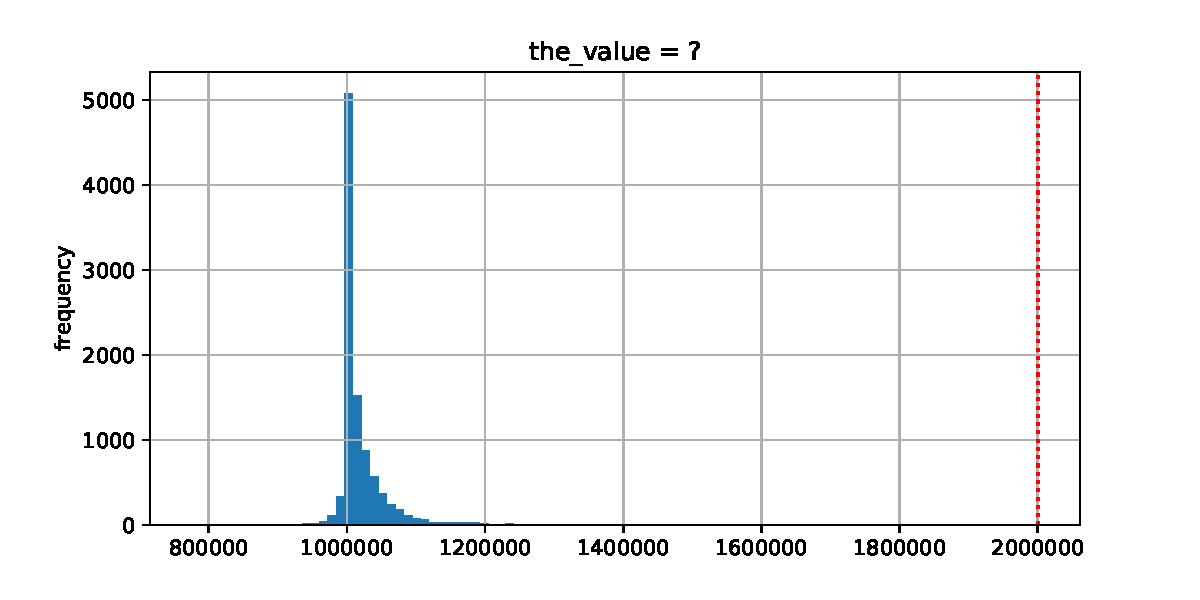
\includegraphics[width=1.1\textwidth]{../sync/parallel-add-histogram}
\end{frame}

\begin{frame}{but how?}
    \begin{itemize}
    \item probably not possible on single core
        \begin{itemize}
            \item exceptions can't occur in the middle of \texttt{add} instruction
        \end{itemize}
    \item \ldots but `add to memory' implemented with multiple steps
        \begin{itemize}
        \item still needs to load, add, store internally
        \item can be interleaved with what other cores do
        \end{itemize}
        \vspace{.5cm}
    \item<2-> {\small (and actually it's more complicated than that --- we'll talk later)}
    \end{itemize}
\end{frame}



\subsection{what is atomic?}

\begin{frame}{so, what is actually atomic}
    \begin{itemize}
    \item for now we'll assume: load/stores of `words' 
        \begin{itemize}
        \item  (64-bit machine = 64-bits words)
        \end{itemize}
        \vspace{.5cm}
    \item in general: \myemph{processor designer will tell you}
    \item their job to design caches, etc. to work as documented
    \end{itemize}
\end{frame}


\section{revisiting atomicity}
\subsection{compiler reordering}
\begin{frame}[fragile,label=compReorder]{compilers move loads/stores (1)}
\begin{lstlisting}[language=C++,style=small,
    moredelim={**[is][\btHL<2|handout:2>]{@2}{2@}},
    moredelim={**[is][\btHL<3|handout:3>]{@3}{3@}},
    moredelim={**[is][\btHL<4|handout:4>]{@4}{4@}},
    moredelim={**[is][\btHL<5|handout:5>]{@5}{5@}},
]
void Alice() {
    note_from_alice = 1;
    @2do {} while (note_from_bob);2@
    if (no_milk) {++milk;}
}
\end{lstlisting}
\hrule
\begin{lstlisting}[language=myasm,style=small,
    moredelim={**[is][\btHL<2|handout:2>]{@2}{2@}},
    moredelim={**[is][\btHL<3|handout:3>]{@3}{3@}},
    moredelim={**[is][\btHL<4|handout:4>]{@4}{4@}},
    moredelim={**[is][\btHL<5|handout:5>]{@5}{5@}},
]
Alice:
  movl $1, note_from_alice  // note_from_alice <- 1
  movl note_from_bob, %eax  // eax <- note_from_bob
.L2:
  @2testl %eax, %eax2@
  @2jne .L22@                   // while (eax == 0) repeat
  cmpl $0, no_milk          // if (no_milk != 0) ...
  ...
\end{lstlisting}
\end{frame}

\begin{frame}[fragile,label=compReorder2]{compilers move loads/stores too (2)}
\begin{lstlisting}[language=C++,style=small,
    moredelim={**[is][\btHL<2|handout:2>]{@2}{2@}},
    moredelim={**[is][\btHL<3|handout:3>]{@3}{3@}},
    moredelim={**[is][\btHL<4|handout:4>]{@4}{4@}},
    moredelim={**[is][\btHL<5|handout:5>]{@5}{5@}},
]
void Alice() {
    @3note_from_alice = 1;3@  // "Alice waiting" signal for Bob()
    do {} while (note_from_bob);
    if (no_milk) {++milk;}
    @2note_from_alice = 2;2@
}
\end{lstlisting}
\hrule
\begin{lstlisting}[language=myasm,style=small,
    moredelim={**[is][\btHL<2|handout:2>]{@2}{2@}},
    moredelim={**[is][\btHL<3|handout:3>]{@3}{3@}},
    moredelim={**[is][\btHL<4|handout:4>]{@4}{4@}},
    moredelim={**[is][\btHL<5|handout:5>]{@5}{5@}},
]
Alice:  
  // compiler optimization: don't set note_from_alice to 1,
  // (why? it will be set to 2 anyway)
  @3movl note_from_bob, %eax3@  // eax <- note_from_bob
.L2:
  testl %eax, %eax          
  jne .L2                   // while (eax == 0) repeat
  ...
  @2movl $2, note_from_alice2@  // note_from_alice <- 2
\end{lstlisting}
\end{frame}


\subsection{fix compiler reordering}
\begin{frame}{fixing compiler reordering?}
    \begin{itemize}
    \item isn't there a way to tell compiler not to do these optimizations?
    \item yes, but that is \myemph{still not enough}!
    \item \textbf{processors} sometimes do this kind of reordering too (between cores)
    \end{itemize}
\end{frame}

\section{pthreads and load/store reordering}
\begin{frame}{pthreads and reordering}
    \begin{itemize}
    \item many pthreads functions \myemph{prevent reordering}
        \begin{itemize}
        \item everything before function call actually happens before 
        \end{itemize}
    \item includes \myemph{preventing some optimizations}
        \begin{itemize}
        \item e.g. keeping global variable in register for too long
        \end{itemize}
    \vspace{.5cm}
    \item pthread\_create, pthread\_join, other tools we'll talk about \ldots
        \begin{itemize}
        \item basically: if pthreads is waiting for/starting something, no weird ordering
        \end{itemize}
    \item implementation part 1: prevent compiler reordering
    \item implementation part 2: use special instructions
        \begin{itemize}
        \item example: x86 \texttt{mfence} instruction
        \end{itemize}
    \end{itemize}
\end{frame}



\section{definitions: mutual exclusion, critical section}
\begin{frame}{some definitions}
\begin{itemize}
\item \textbf{mutual exclusion}: ensuring only one thread does a particular thing at a time
    \begin{itemize}
        \item like updating shared balance
    \end{itemize}
\item<2-> \textbf{critical section}: code that exactly one thread can execute at a time
    \begin{itemize}
        \item result of mutual exclusion
    \end{itemize}
\item<3-> \textbf{lock}: object only one thread can hold at a time
    \begin{itemize}
        \item interface for creating critical sections
    \end{itemize}
\end{itemize}
\end{frame}


\section{locks}
\begin{frame}{lock analogy}
    \begin{itemize}
    \item agreement: whoever holds the flag can access shared resource
        \begin{itemize}
        \item flag doesn't actually do anything by itself\ldots
        \end{itemize}
    \item acquire/lock $\approx$ wait for and grab flag from table
    \item release/unlock $\approx$ put flag back on table
    \vspace{.5cm}
    \item<2-> agreement is \myemph{voluntary}
        \begin{itemize}
        \item thread tries to manipulate shared resource without lock? \\
            lock won't stop it\ldots
        \end{itemize}
    \item<2-> lock is \textit{held} by particular thread
    \end{itemize}
\end{frame}


% FIXME: lock analogy: hat
\begin{frame}[fragile,label=lockDefn]{the lock primitive}
    \begin{itemize}
    \item locks: an object with (at least) two operations:
        \begin{itemize}
        \item \textit{acquire} or \textit{lock} --- wait until lock is free, then ``grab'' it
        \item \textit{release} or \textit{unlock} --- let others use lock, wakeup waiters
        \end{itemize}
    \item typical usage: everyone acquires lock before using shared resource
        \begin{itemize}
        \item forget to acquire lock? weird things happen
        \end{itemize}
    \end{itemize}
\begin{lstlisting}[language=C++,style=small]
Lock(account_lock);
balance += ...;
Unlock(account_lock);
\end{lstlisting}
\end{frame}


\begin{frame}[fragile,label=pthreadMutex]{pthread mutex}
\begin{lstlisting}[language=C++,style=small]
#include <pthread.h>

pthread_mutex_t account_lock;
pthread_mutex_init(&account_lock, NULL);
    // or: pthread_mutex_t account_lock =
    //              PTHREAD_MUTEX_INITIALIZER;
...
pthread_mutex_lock(&account_lock);
balance += ...;
pthread_mutex_unlock(&account_lock;
\end{lstlisting}
\end{frame}



\subsection{exercise}
\begin{frame}[fragile,label=lockEx]{exercise}
    \vspace{-0.5cm}
\begin{lstlisting}[style=smaller]
pthread_mutex_t lock1 = PTHREAD_MUTEX_INITIALIZER;
pthread_mutex_t lock2 = PTHREAD_MUTEX_INITIALIZER;
string one = "init one", two = "init two";
void ThreadA() {
    pthread_mutex_lock(&lock1);
    one = "one in ThreadA";  // (A1)
    pthread_mutex_unlock(&lock1);
    pthread_mutex_lock(&lock2);
    two = "two in ThreadA";  // (A2)
    pthread_mutex_unlock(&lock2);
}
void ThreadB() {
    pthread_mutex_lock(&lock1);
    one = "one in ThreadB";  // (B1)
    pthread_mutex_lock(&lock2);
    two = "two in ThreadB";  // (B2)
    pthread_mutex_unlock(&lock2);
    pthread_mutex_unlock(&lock1);
}
\end{lstlisting}
possible values of one/two after A+B run?
\end{frame}

\begin{frame}<0>[fragile,label=lockExSln]{solution}
\begin{itemize}
\item B1+A2
    \begin{itemize}
    \item A: L(1) A1 U(1) L
    \item B: L(1) B1 L(2) B2 U(2) U(1)
    \item A: L(2) A2 U(2)
    \end{itemize}
\item NOT A1+B2
    \begin{itemize}
    \item would need to run B1 after A1 before A2
    \item not possible because Lock1 held for entire B1+B2 operation
    \item \ldots and A1 needs Lock1, too
    \end{iteimze}
\end{itemize}
\end{frame}

\begin{frame}[fragile,label=lockExAlt1]{exercise (alternate 1)}
    \vspace{-0.5cm}
\begin{lstlisting}[style=smaller]
pthread_mutex_t lock1 = PTHREAD_MUTEX_INITIALIZER;
pthread_mutex_t lock2 = PTHREAD_MUTEX_INITIALIZER;
string one = "init one", two = "init two";
void ThreadA() {
    pthread_mutex_lock(&lock2);
    two = "two in ThreadA";  // (A2)
    pthread_mutex_unlock(&lock2);
    pthread_mutex_lock(&lock1);
    one = "one in ThreadA";  // (A1)
    pthread_mutex_unlock(&lock1);
}
void ThreadB() {
    pthread_mutex_lock(&lock1);
    one = "one in ThreadB";  // (B1)
    pthread_mutex_lock(&lock2);
    two = "two in ThreadB";  // (B2)
    pthread_mutex_unlock(&lock2);
    pthread_mutex_unlock(&lock1);
}
\end{lstlisting}
possible values of one/two after A+B run?
\end{frame}

\begin{frame}[fragile,label=lockExAlt2]{exercise (alternate 2)}
    \vspace{-0.5cm}
\begin{lstlisting}[style=smaller]
pthread_mutex_t lock1 = PTHREAD_MUTEX_INITIALIZER;
pthread_mutex_t lock2 = PTHREAD_MUTEX_INITIALIZER;
string one = "init one", two = "init two";
void ThreadA() {
    pthread_mutex_lock(&lock2);
    two = "two in ThreadA";  // (A2)
    pthread_mutex_unlock(&lock2);
    pthread_mutex_lock(&lock1);
    one = "one in ThreadA";  // (A1)
    pthread_mutex_unlock(&lock1);
}
void ThreadB() {
    pthread_mutex_lock(&lock1);
    one = "one in ThreadB";  // (B1)
    pthread_mutex_unlock(&lock1);
    pthread_mutex_lock(&lock2);
    two = "two in ThreadB";  // (B2)
    pthread_mutex_unlock(&lock2);
}
\end{lstlisting}
possible values of one/two after A+B run?
\end{frame}


\subsection{pthread\_mutex: lock where you unlock}
\begin{frame}{POSIX mutex restrictions}
\begin{itemize}
\item pthread\_mutex rule: \myemph{unlock from same thread you lock in}
\vspace{.5cm}
\item does this actually matter?
\item depends on how pthread\_mutex is implemented
\end{itemize}
\end{frame}


\section{preview: more advance sync}
\begin{frame}{preview: general sync}
    \begin{itemize}
    \item lots of coordinating threads beyond locks/barriers
    \item will talk about two general tools later:
        \begin{itemize}
        \item monitors/condition variables
        \item semaphores
        \end{itemize}
    \item big added feature: wait for arbitrary thing to happen
    \end{itemize}
\end{frame}

\begin{frame}[fragile]{a bad idea}
\begin{itemize}
\item one \myemph{bad} idea to wait for an event:
\end{itemize}
\begin{lstlisting}
bool happened = false;
void WaitForEvent() {
    do {} while (!happened);
}

void EventHappened() {
    happened = true;
}
\end{lstlisting}
\begin{itemize}
\item wastes processor time
\item and also \myemph{doesn't work!}
\end{itemize}
\end{frame}


\subsection{beyond locks}
\begin{frame}[fragile,label=beyondLock]{beyond locks}
    \begin{itemize}
    \item in practice: want more than locks for synchronization
    \item for waiting for arbtirary events (without CPU-hogging-loop):
        \begin{itemize}
        \item monitors
        \item semaphores
        \end{itemize}
    \item for common synchornization patterns:
        \begin{itemize}
        \item barriers
        \item reader-writer locks
        \end{itemize}
    \item higher-level interface:
        \begin{itemize}
        \item transactions
        \end{itemize}
    \end{itemize}
\end{frame}


\usetikzlibrary{arrows.meta,shapes.geometric}
\tikzset{
    >=Latex,
    resource/.style={draw,rectangle,very thick,align=center},
    resource m/.style={draw,rectangle,very thick,align=center,row sep=2mm},
    resource circle/.style={circle,fill=black,inner sep=0mm,minimum width=2.5mm},
    thread/.style={draw,ellipse,very thick,align=center},
    dependency/.style={draw,ultra thick,->},
    dependency future/.style={dependency,dotted},
    dependency reason/.style={align=center},
}


\section{deadlock examples}

\subsection{a one-way bridge}
\begin{frame}{the one-way bridge}
\begin{tikzpicture}
\tikzset{
    bridge line/.style={ultra thick},
    road divide/.style={very thick,loosely dashed},
    old car black/.pic={
        \node at (0,-0.25) {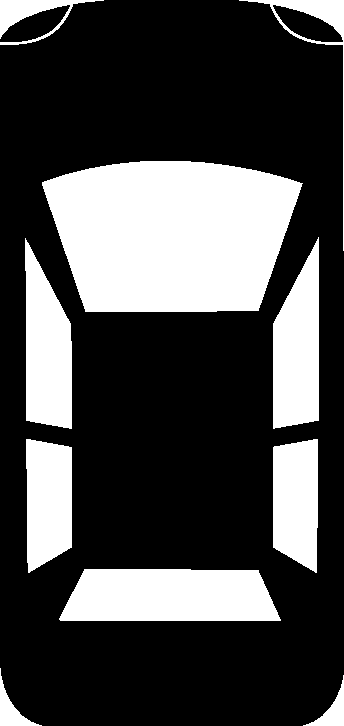
\includegraphics[width=1.25cm,angle=-90,origin=c]{../deadlock/Car_icon_top.pdf}};
    },
    old car black opposite/.pic={
        \node at (0,-0.25) {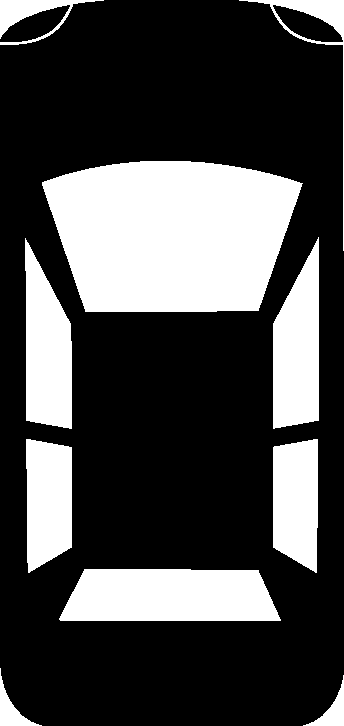
\includegraphics[width=1.25cm,angle=90,origin=c]{../deadlock/Car_icon_top.pdf}};
    },
    old car black opposite rot/.pic={
        \node at (0,-0.25) {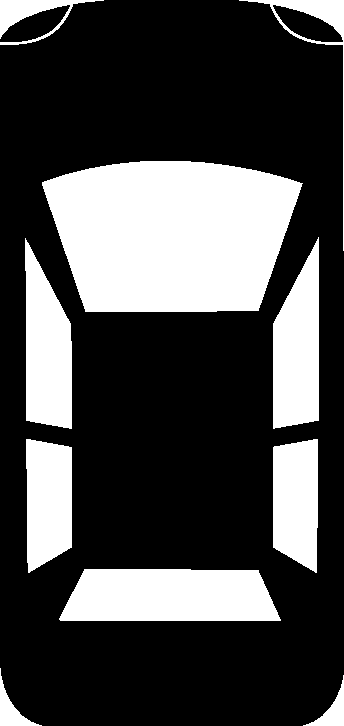
\includegraphics[width=1.25cm,angle=85,origin=c]{../deadlock/Car_icon_top.pdf}};
    },
    old car red/.pic={
        \node at (0,-0.25) {
\includegraphics[width=1.25cm,angle=-90,origin=c]{../deadlock/Car_red.pdf}};
    },
    old car red rot/.pic={
        \node at (0,-0.25) {
\includegraphics[width=1.25cm,angle=-100,origin=c]{../deadlock/Car_red.pdf}};
    },
    car black opposite/.pic={
        \node at (0,-0.25) {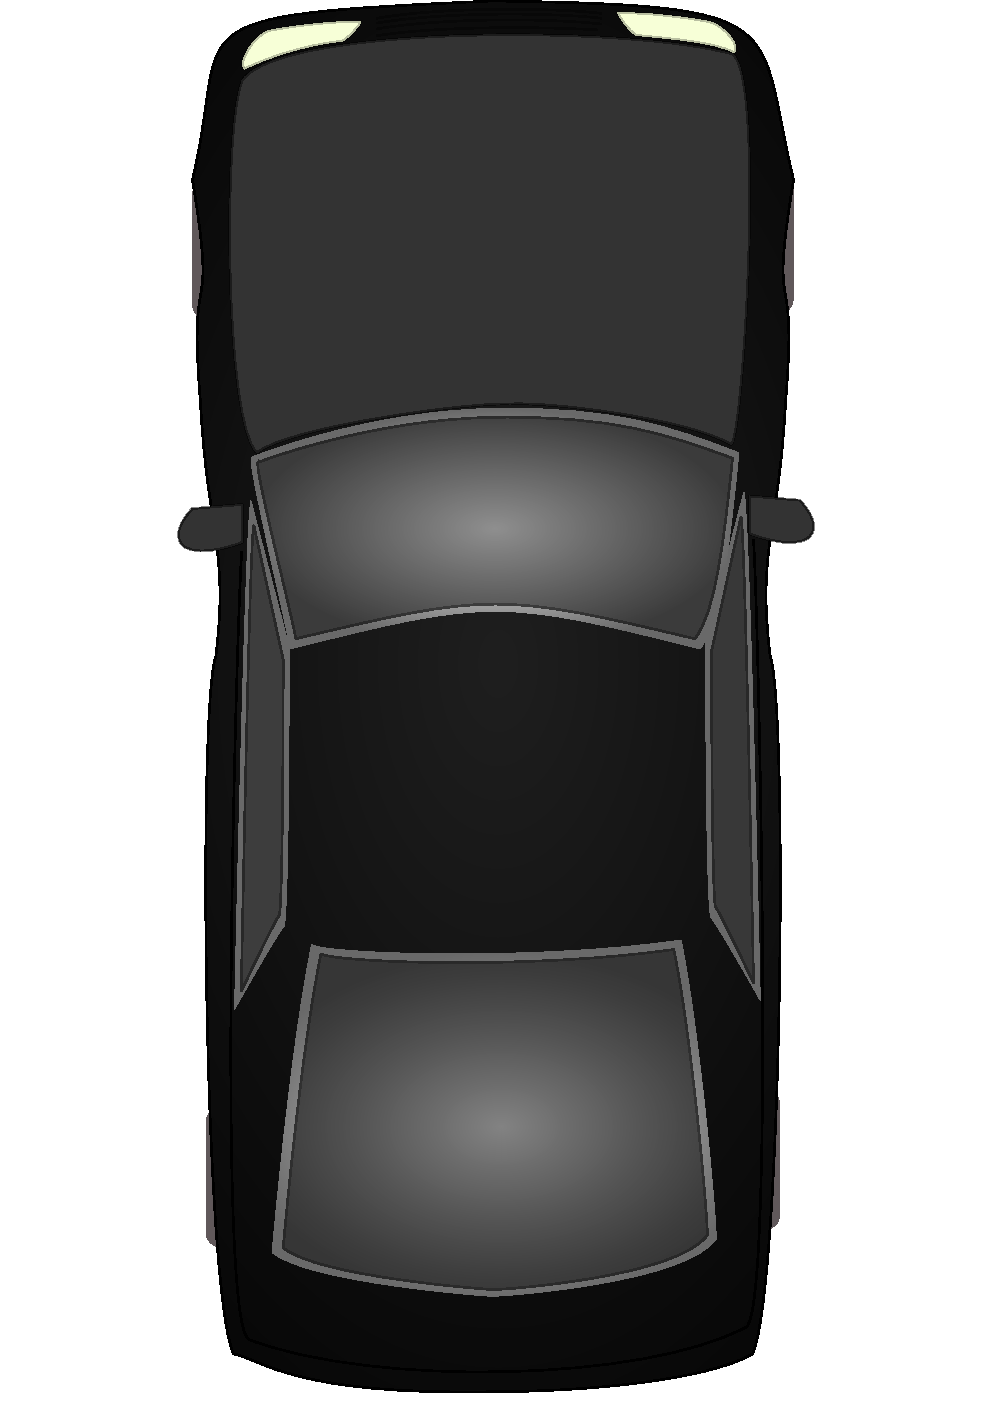
\includegraphics[width=2cm,angle=90,origin=c]{../deadlock/car-black.pdf}};
    },
    car black opposite rot/.pic={
        \node at (0,-0.25) {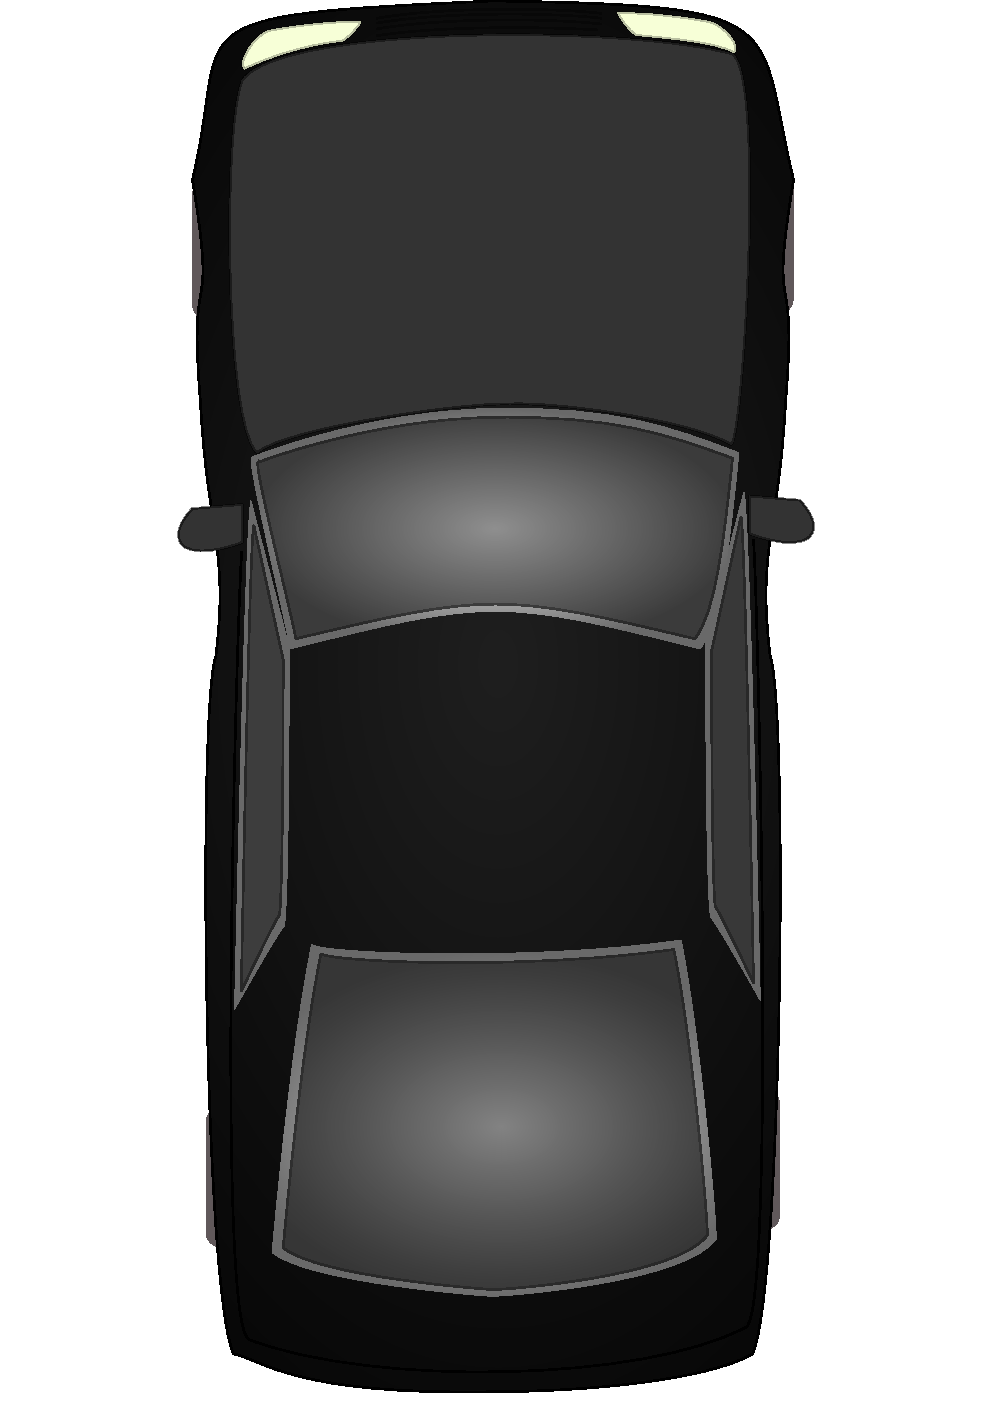
\includegraphics[width=2cm,angle=85,origin=c]{../deadlock/car-black.pdf}};
    },
    car yellow/.pic={
        \node at (0,-0.25) {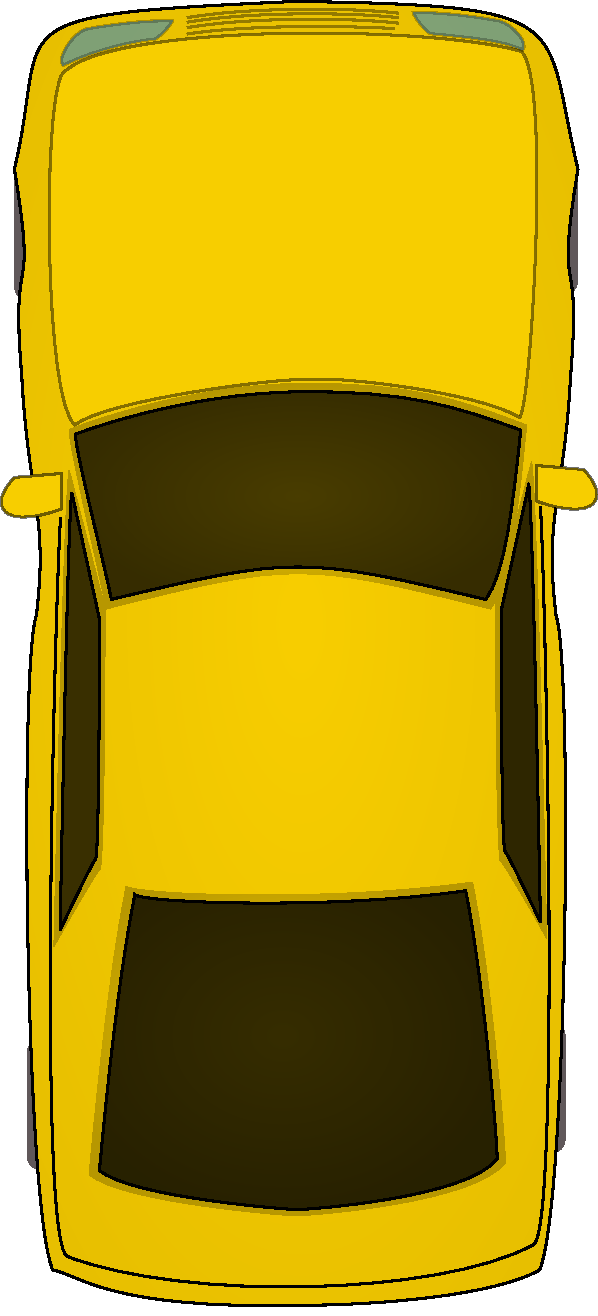
\includegraphics[width=1.25cm,angle=-90,origin=c]{../deadlock/car-yellow.pdf}};
    },
    car yellow rot/.pic={
        \node at (0,-0.25) {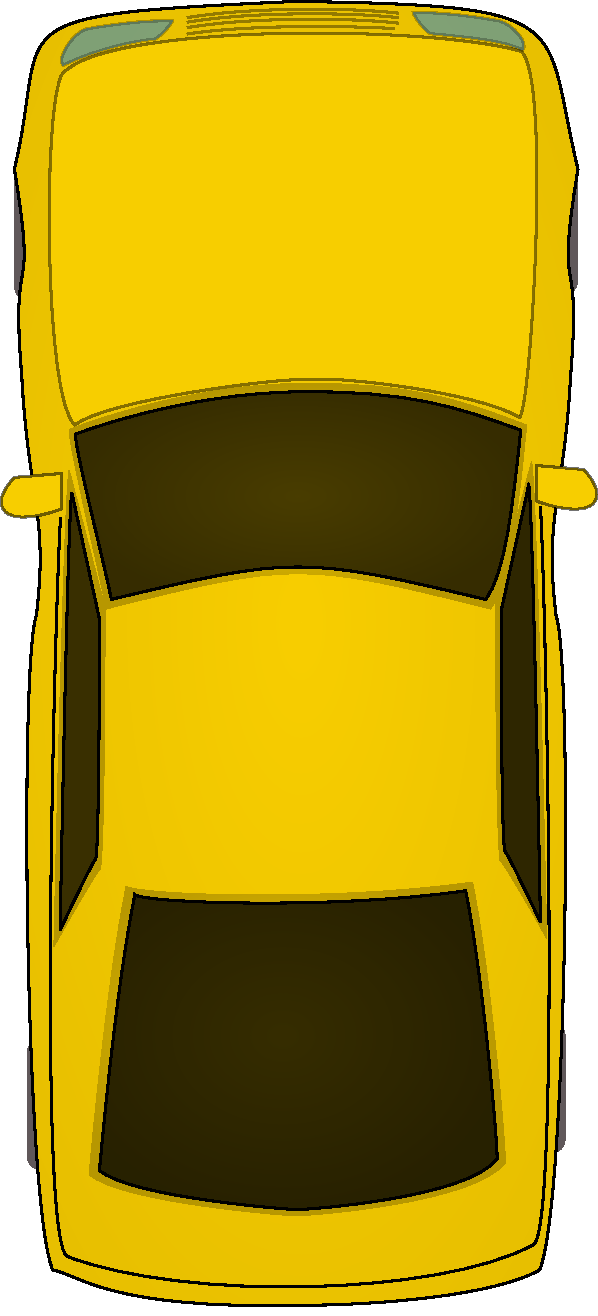
\includegraphics[width=1.25cm,angle=-100,origin=c]{../deadlock/car-yellow.pdf}};
    },
}
\draw[bridge line] (-4.5, -1) -- (-1, -1) -- (1, 0) -- (5, 0) -- (7, -1) -- (10.5, -1);
\draw[bridge line] (-4.5, 3) -- (-1, 3) -- (1, 2) -- (5, 2) -- (7, 3) -- (10.5, 3);
\draw[road divide] (-4.5, 1) -- (-1.5, 1);
\draw[road divide] (7.5, 1) -- (10.5, 1);

\begin{visibleenv}<1-2>
\path[overlay] (-3, 2) pic{car yellow};
\path[overlay] (9.5, 0) pic{car black opposite};
\end{visibleenv}

\begin{pgfonlayer}{bg}
\begin{visibleenv}<2>
\path[fill=yellow!60!black!20] (-1.5, 1) -- (-1.5, 3) -- (-1, 3) -- (1, 2) -- (2.5, 2) -- (2.5, 0) -- (1, 0) -- (-1, 1) -- cycle;
\end{visibleenv}
\begin{visibleenv}<2>
\path[fill=black!30] (8.0, 1) -- (8, -1) -- (7, -1) -- (5, 0) -- (4, 0) -- (4, 2) -- (5, 2) -- (7, 1) -- cycle;
\end{visibleenv}
\end{pgfonlayer}

\begin{visibleenv}<3-4>
\path[overlay] (1, 1.2) pic{car yellow rot};
\path[overlay] (5, 1) pic{car black opposite rot};
\end{visibleenv}

\end{tikzpicture}
\end{frame}


\subsection{with locks}
\usetikzlibrary{matrix}

\begin{frame}[fragile,label=moveFileDeadlock]{moving two files}
\begin{lstlisting}[language=C++,style=smaller]
struct Dir {
  mutex_t lock; map<string, DirEntry> entries;
};
void MoveFile(Dir *from_dir, Dir *to_dir, string filename) {
  mutex_lock(&from_dir->lock);
  mutex_lock(&to_dir->lock);
    
  to_dir->entries[filename] = from_dir->entries[filename];
  from_dir->entries.erase(filename);

  mutex_unlock(&to_dir->lock);
  mutex_unlock(&from_dir->lock);
}
\end{lstlisting}
Thread 1: \texttt{MoveFile(A, B, "foo")} \\
Thread 2: \texttt{MoveFile(B, A, "bar")} 
\end{frame}

\begin{frame}[fragile,label=moveFileNoDeadlockTimeline1]{moving two files: lucky timeline (1)}
\begin{tikzpicture}
\tikzset{
  timeline/.style={
    tight matrix no line,
    ampersand replacement=\Q,
    nodes={text width=7cm,
      minimum height=0.6cm,
        font=\small\tt\lstset{language=C++,style=small},
        },
    column sep=1cm,
    row 1/.style={nodes={font=\bfseries,align=center}},
    row 2/.style={nodes={font=\bfseries\tt}},
  },
  waiting/.style={text=black!40},
}
\matrix[timeline] (timeline) {
  Thread 1 \Q Thread 2 \\
  MoveFile(A, B, "foo") \Q MoveFile(B, A, "bar") \\
  {lock(\&A->lock);} \\
  {lock(\&B->lock);} \\
  {\normalfont (do move)} \\
  {unlock(\&B->lock);} \\
  {unlock(\&A->lock);} \\
  \Q {lock(\&B->lock);} \\
  \Q {lock(\&A->lock);} \\
  \Q {\normalfont (do move)} \\
  \Q {unlock(\&B->lock);} \\
  \Q {unlock(\&A->lock);} \\
};
\draw[very thick] (timeline-2-1.south west) -- (timeline-2-2.south east);
\end{tikzpicture}
\end{frame}

\begin{frame}[fragile,label=moveFileNoDeadlockTimeline2]{moving two files: lucky timeline (2)}
\begin{tikzpicture}
\tikzset{
  timeline/.style={
    tight matrix no line,
    ampersand replacement=\Q,
    nodes={text width=7cm,
      minimum height=0.6cm,
        font=\small\tt\lstset{language=C++,style=small},
        },
    column sep=1cm,
    row 1/.style={nodes={font=\bfseries,align=center}},
    row 2/.style={nodes={font=\bfseries\tt}},
  },
  waiting/.style={text=black!40},
}
\matrix[timeline] (timeline) {
  Thread 1 \Q Thread 2 \\
  MoveFile(A, B, "foo") \Q MoveFile(B, A, "bar") \\
  {lock(\&A->lock);} \Q \\
  {lock(\&B->lock);} \Q \\
  \Q |[waiting]| {lock(\&B->lock\ldots} \\
  {\normalfont (do move)} \Q |[waiting]|  {\normalfont (waiting for B lock)} \\
  {unlock(\&B->lock);} \\
  \Q {lock(\&B->lock);} \\
  \Q |[waiting]| {lock(\&A->lock\ldots} \\
  {unlock(\&A->lock);} \\
  \Q {lock(\&A->lock);} \\
  \Q {\normalfont (do move)} \\
  \Q {unlock(\&A->lock);} \\
  \Q {unlock(\&B->lock);} \\
};
\draw[very thick] (timeline-2-1.south west) -- (timeline-2-2.south east);
\end{tikzpicture}
\end{frame}

\begin{frame}[fragile,label=moveFileDeadlockTimeline]{moving two files: unlucky timeline}
\begin{tikzpicture}
\tikzset{
  timeline/.style={
    tight matrix no line,
    ampersand replacement=\Q,
    nodes={text width=7cm,
      minimum height=0.6cm,
        font=\small\tt\lstset{language=C++,style=small},
        },
    column sep=1cm,
    row 1/.style={nodes={font=\bfseries,align=center}},
    row 2/.style={nodes={font=\bfseries\tt}},
  },
  waiting/.style={text=black!40},
}
\matrix[timeline] (timeline) {
  Thread 1 \Q Thread 2 \\
  MoveFile(A, B, "foo") \Q MoveFile(B, A, "bar") \\
  {lock(\&A->lock);} \Q \\
  \Q {lock(\&B->lock);} \\
  {lock(\&B->lock\ldots \normalfont{ \myemph{stalled}}} \Q \\
  |[waiting]| \normalfont (waiting for lock on B) \Q {lock(\&A->lock\ldots \normalfont{ \myemph{stalled}}} \\
  |[waiting]| \normalfont (waiting for lock on B) \Q |[waiting]| \normalfont (waiting for lock on A) \\
  ~ \Q ~ \\
  \normalfont{\sout{(do move)}{ }\myemph{unreachable}} \Q \normalfont{\sout{(do move)}{ }\myemph{unreachable}} \\
  \sout{unlock(\&B->lock);}\normalfont{ \myemph{unreachable}} \Q \sout{unlock(\&A->lock);} \normalfont{ \myemph{unreachable}} \\
  \sout{unlock(\&A->lock);}\normalfont{ \myemph{unreachable}} \Q\sout{unlock(\&B->lock);} \normalfont{ \myemph{unreachable}} \\
};
\draw[very thick] (timeline-2-1.south west) -- (timeline-2-2.south east);
\begin{visibleenv}<1|handout:0>
\fill[white] (timeline-5-1.north west) rectangle (timeline.south east);
\end{visibleenv}
\begin{visibleenv}<2|handout:0>
\fill[white] (timeline-8-1.north west) rectangle (timeline.south east);
\end{visibleenv}
\begin{visibleenv}<4->
\node[anchor=north,align=center] at ([yshift=-.5cm]timeline.south) {
Thread 1 holds A lock, waiting for Thread 2 to release B lock \\
Thread 2 holds B lock, waiting for Thread 1 to release A lock 
};
\end{visibleenv}
\end{tikzpicture}
\end{frame}

\usetikzlibrary{arrows.meta,shapes.geometric}
\tikzset{
    >=Latex,
    resource/.style={draw,rectangle,very thick,align=center},
    resource m/.style={draw,rectangle,very thick,align=center,row sep=2mm},
    resource circle/.style={circle,fill=black,inner sep=0mm,minimum width=2.5mm},
    thread/.style={draw,ellipse,very thick,align=center},
    dependency/.style={draw,ultra thick,->},
    dependency future/.style={dependency,dotted},
    dependency reason/.style={align=center},
}

\begin{frame}{moving two files: dependencies}
\begin{tikzpicture}
\node[resource] (directory A) {
    directory B 
};
\node[resource] (directory B) at ([yshift=-6cm]directory A) {
    directory A
};
\node[thread] (thread one) at ([xshift=-4cm,yshift=-3cm]directory A) {
  thread 1
};
\node[thread] (thread two) at ([xshift=4cm,yshift=-3cm]directory A) {
  thread 2
};

\path[dependency] (thread one.north) ..  controls ([yshift=2cm]thread one.north) .. (directory A.west)
    node[midway,dependency reason,left] {
      waiting for lock
    };
\path[dependency] (thread two.south) ..  controls ([yshift=-2cm]thread two.south) .. (directory B.east)
    node[midway,dependency reason,right] {
      waiting for lock
    };
\path[dependency future] (directory A.east) .. controls ([yshift=2cm]thread two.north) .. (thread two.north)
    node[midway,dependency reason,right] {
      lock held by
    };
\path[dependency future] (directory B.west) .. controls ([yshift=-2cm]thread one.south) .. (thread one.south)
    node[midway,dependency reason,left] {
      lock held by
    };
\end{tikzpicture}
\end{frame}

\begin{frame}{moving three files: dependencies}
\begin{tikzpicture}
\node[resource] (directory A) {
    directory B 
};
\node[resource] (directory B) at ([yshift=-4cm,xshift=4cm]directory A) {
    directory C
};
\node[resource] (directory C) at ([yshift=-4cm,xshift=-4cm]directory A) {
    directory A
};
\node[thread] (thread one) at ([xshift=-4cm,yshift=-1.5cm]directory A) {
  thread 1
};
\node[thread] (thread two) at ([xshift=4cm,yshift=-1.5cm]directory A) {
  thread 2
};
\node[thread] (thread three) at ([yshift=-6cm]directory A) {
  thread 3
};

\path[dependency] (thread one.north) ..  controls ([yshift=1cm]thread one.north) .. (directory A.west)
    node[midway,dependency reason,left] {
      waiting for lock
    };
\path[dependency] (thread two.south) ..  controls ([yshift=-1cm]thread two.south) .. (directory B.north)
    node[midway,dependency reason,right] {
      waiting for lock
    };
\path[dependency] (thread three.west) ..  controls ([yshift=-1cm]directory C.south) .. (directory C.south)
    node[midway,dependency reason,below left] {
      waiting for lock
    };
\path[dependency future] (directory A.east) .. controls ([yshift=1cm]thread two.north) .. (thread two.north)
    node[midway,dependency reason,right] {
      lock held by
    };
\path[dependency future] (directory B.south) .. controls ([xshift=2cm]thread three.east) .. (thread three.east)
    node[midway,dependency reason,below right] {
      lock held by
    };
\path[dependency future] (directory C.north) .. controls ([yshift=-1cm]thread one.south) .. (thread one.south)
    node[midway,dependency reason,left] {
      lock held by
    };
\end{tikzpicture}
\end{frame}

\begin{frame}[fragile,label=moveFileDeadlockTimeline2]{moving three files: unlucky timeline}
\begin{tikzpicture}
\tikzset{
  timeline/.style={
    tight matrix no line,
    ampersand replacement=\Q,
    nodes={text width=4.5cm,
      minimum height=0.6cm,
        font=\fontsize{9.5}{10.5}\selectfont\tt\lstset{language=C++,style=small},
        },
    column sep=0.25cm,
    row 1/.style={nodes={font=\fontsize{10}{11}\selectfont\bfseries,align=center}},
    row 2/.style={nodes={font=\fontsize{10}{11}\selectfont\bfseries\tt}},
  waiting/.style={text=black!40},
  },
}
\matrix[timeline] (timeline) {
  Thread 1 \Q Thread 2 \Q Thread 3\\
  MoveFile(A, B, "foo") \Q MoveFile(B, C, "bar") \Q MoveFile(C, A, "quux") \\
  {lock(\&A->lock);} \Q ~ \Q ~\\
  \Q {lock(\&B->lock);} \\
  \Q \Q {lock(\&C->lock);} \\
  {lock(\&B->lock\ldots}{ }\normalfont{\myemph{stalled}} \Q \\
  \Q {lock(\&C->lock\ldots}{ }\normalfont{\myemph{stalled}} \\
  \Q \Q {lock(\&A->lock\ldots}{ }\normalfont{\myemph{stalled}} \\
};
\begin{scope}[red!70!black]
\draw[dashed,-Latex,thick,in=-90] ([xshift=-.75cm]timeline-6-1.east) to (timeline-4-2.south);
\draw[dashed,-Latex,thick,in=-90] ([xshift=-.75cm]timeline-7-2.east) to (timeline-5-3.south);
\draw[dashed,-Latex,thick] ([xshift=-.75cm]timeline-8-3.east) to[out=0,in=0] (timeline-3-3.center) to ([xshift=-1cm]timeline-3-1.east);
\end{scope}
\end{tikzpicture}
\end{frame}


\subsection{with memory}
\begin{frame}{deadlock with free space}
\begin{tikzpicture}
\tikzset{
  timeline/.style={
    tight matrix no line,
    ampersand replacement=\Q,
    nodes={text width=7cm,
      minimum height=0.6cm,
        font=\small\tt\lstset{language=C++,style=small},
        },
    column sep=1cm,
    row 1/.style={nodes={font=\bfseries,align=center}},
  },
  waiting/.style={text=black!40},
}
\matrix[timeline] (timeline) {
  Thread 1 \Q Thread 2 \\
  AllocateOrWaitFor(1 MB) \Q AllocateOrWaitFor(1 MB) \\
  AllocateOrWaitFor(1 MB) \Q AllocateOrWaitFor(1 MB) \\
  (do calculation) \Q (do calculation) \\
  Free(1 MB) \Q Free(1 MB) \\
  Free(1 MB) \Q Free(1 MB) \\
};
\node[anchor=north,align=center] at (timeline.south) { 
  2 MB of space --- deadlock possible with unlucky order
};
\end{tikzpicture}
\end{frame}

\begin{frame}{deadlock with free space (unlucky case)}
\begin{tikzpicture}
\tikzset{
  timeline/.style={
    tight matrix no line,
    ampersand replacement=\Q,
    nodes={text width=7cm,
      minimum height=0.6cm,
        font=\small\tt\lstset{language=C++,style=small},
        },
    column sep=1cm,
    row 1/.style={nodes={font=\bfseries,align=center}},
  },
  waiting/.style={text=black!40},
}
\matrix[timeline] (timeline) {
  Thread 1 \Q Thread 2 \\
  AllocateOrWaitFor(1 MB) \\
  \Q  AllocateOrWaitFor(1 MB) \\
  AllocateOrWaitFor(1 MB\ldots{ }\normalfont{\myemph{stalled}} \\
  \Q AllocateOrWaitFor(1 MB\ldots{ }\normalfont{\myemph{stalled}} \\
};
\node[anchor=north,align=center] at (timeline.south) { 

};
\end{tikzpicture}
\end{frame}

\begin{frame}[fragile,label=freeSpaceDepend]{free space: dependency graph}
\begin{tikzpicture}
    \newcommand{\mycircle}[1]{
        \node[resource circle] (#1) {};
    }
    \matrix[resource,row sep=2mm,label={[align=left,xshift=-1cm]north east:{memory in \\2 (1MB) units}}] (resource A) {
    \mycircle{A one} \\
    \mycircle{A two} \\
};
\node[thread] (thread one) at ([xshift=-3cm,yshift=-3cm]resource A) {
  thread 1
};
\node[thread] (thread two) at ([xshift=3cm,yshift=-3cm]resource A) {
  thread 2
};
    \path[dependency future] (A one.west) .. controls ([xshift=-1cm]A one.west) .. (thread one.north)
        node[pos=0.8,above] {allocated};
    \path[dependency future] (A two.east) .. controls ([xshift=1cm]A two.east) .. (thread two.north);
    \path[dependency] (thread one.east) .. controls ([xshift=1cm]thread one.east) .. (resource A.south)
        node[midway,below=.5cm,xshift=1cm] {waiting for};
    \path[dependency] (thread two.west) .. controls ([xshift=-1cm]thread two.west) .. (resource A.south);
\end{tikzpicture}
\end{frame}

\begin{frame}{deadlock with free space (lucky case)}
\begin{tikzpicture}
\tikzset{
  timeline/.style={
    tight matrix no line,
    ampersand replacement=\Q,
    nodes={text width=7cm,
      minimum height=0.6cm,
        font=\small\tt\lstset{language=C++,style=small},
        },
    column sep=1cm,
    row 1/.style={nodes={font=\bfseries,align=center}},
  },
  waiting/.style={text=black!40},
}
\matrix[timeline] (timeline) {
  Thread 1 \Q Thread 2 \\
  AllocateOrWaitFor(1 MB) \\
  AllocateOrWaitFor(1 MB) \\
  (do calculation) \\
  Free(1 MB); \\ 
  Free(1 MB); \\
  \Q AllocateOrWaitFor(1 MB) \\
  \Q AllocateOrWaitFor(1 MB) \\
  \Q (do calculation) \\
  \Q Free(1 MB); \\ 
  \Q Free(1 MB); \\
};
\end{tikzpicture}
\end{frame}

 
\section{deadlock definition}

\subsection{short intuition}

\begin{frame}{deadlock}
\begin{itemize}
\item deadlock --- circular waiting for \myemph<2>{resources}
\vspace{.5cm}
\item resource = something needed by a thread to do work
  \begin{itemize}
  \item locks
  \item CPU time
  \item disk space
  \item memory
  \item \ldots
  \end{itemize}
\item often non-deterministic in practice
\item most common example: \myemph{when acquiring multiple locks}
\end{itemize}
\end{frame}

\begin{frame}{deadlock versus starvation}
\begin{itemize}
\item starvation: one+ unlucky (no progress), 
                  one+ lucky (yes progress)
    \begin{itemize}
    \item example: low priority threads versus high-priority threads
    \end{itemize}
\item deadlock: no one involved in deadlock makes progress
\vspace{.5cm}
\item<2-> starvation: once starvation happens, taking turns will resolve
    \begin{itemize}
    \item low priority thread just needed a chance\ldots
    \end{itemize}
\item<2-> deadlock: once it happens, taking turns won't fix
\end{itemize}
\end{frame}


\subsection{conditions for deadlock}

\begin{frame}{deadlock requirements}
\begin{itemize}
\item \textbf{mutual exclusion}
    \begin{itemize}
    \item one thread at a time can use a resource
    \end{itemize}
\item \textbf{hold and wait}
  \begin{itemize}
  \item thread holding a resources waits to acquire \textit{another} resource
  \end{itemize}
\item \textbf{no preemption of resources}
    \begin{itemize}
    \item resources are only released voluntarily
    \item thread trying to acquire resources can't `steal'
    \end{itemize}
\item \textbf{circular wait}
    \begin{itemize}
    \item there exists a set $\{T_1,\ldots,T_n\}$ of waiting threads such that
        \begin{itemize}
        \item $T_1$ is waiting for a resource held by $T_2$
        \item $T_2$ is waiting for a resource held by $T_3$
        \item \ldots
        \item $T_n$ is waiting for a resource held by $T_1$
        \end{itemize}
    \end{itemize}
\end{itemize}
\end{frame}


\section{exercise}

\begin{frame}[fragile,label=isDeadlockP]{how is deadlock possible?}
Given list: A, B, C, D, E
\begin{lstlisting}[style=size10]
RemoveNode(LinkedListNode *node) {
    pthread_mutex_lock(&node->lock);
    pthread_mutex_lock(&node->prev->lock);
    pthread_mutex_lock(&node->next->lock);
    node->next->prev = node->prev; node->prev->next = node->next;
    pthread_mutex_unlock(&node->next->lock); pthread_mutex_unlock(&node->prev->lock);
    pthread_mutex_unlock(&node->lock);
}
\end{lstlisting}
Which of these (all run in parallel) can deadlock? \\
\begin{tabular}{l} 
A. RemoveNode(B) and RemoveNode(C) \\
B. RemoveNode(B) and RemoveNode(D) \\
C. RemoveNode(B) and RemoveNode(C) and RemoveNode(D) \\
D. A and C \hspace{3cm} E. B and C \\
F. all of the above \hspace{1cm} G. none of the above \\
\end{tabular}
\end{frame}

\begin{frame}<0>[label=isDeadlockPTimeline1]{how is deadlock --- solution}
\begin{tabular}{l|l}
Remove B & Remove C \\
lock B & lock C \\
lock A (prev) & wait to lock B (prev) \\
wait to lock C (next) &
\end{tabular}
\hrule
With B and D --- only overlap in in node C --- no circular wait possible
\end{frame}

\iftoggle{heldback}{}{\againframe<1>{isDeadlockPTimeline1}}


\section{deadlock prevention}

\subsection{techniques overview}

\usetikzlibrary{matrix,positioning,shapes.callouts}

\begin{frame}<0>[label=deadlockPrevent]{deadlock prevention techniques}
\begin{tikzpicture}
\matrix[
  tight matrix no line,
  column 1/.style={nodes={text width=10cm,align=left}},
  column 2/.style={nodes={text width=5cm}},
  row sep=.5cm,
] {
{%
  \textbf{\myemph<2>{infinite resources}} \\
  \hspace{1cm}or at least enough that never run out
} \& {no \textit{mutual exclusion}} \\
{%
  \textbf{\myemph<3>{no shared resources}}
} \& {no \textit{mutual exclusion}} \\
|[alias=no wait]| {%
  \textbf{\myemph<4,7,8>{no waiting}} \\
\hspace{1cm} ``\myemph<4,8>{busy signal}'' --- \myemph<4,8>{abort and (maybe) retry} \\
\hspace{1cm} \myemph<7>{revoke/preempt resources}
} \& {no \textit{hold and wait}/\\\textit{preemption}} \\
{%
  acquire resources in \textbf{\myemph<5>{consistent order}}
} \& {no \textit{circular wait}} \\
{%
  request \textbf{\myemph<6>{all resources at once}}
} \& {no \textit{hold and wait}} \\
};
\begin{visibleenv}<4>
\coordinate (abort retry) at ([xshift=-3cm,yshift=-.7cm]no wait.north east);
\node[my callout2=abort retry,anchor=south east,align=left,font=\small] at ([xshift=5cm,yshift=.9cm]abort retry) {
    memory allocation: malloc() fails rather than waiting (no deadlock) \\
    locks: \texttt{pthread\_mutex\_trylock} fails rather than waiting \\
    problem: retry how many times? \myemph{no bound on number of tries needed} \\
    \ldots
};
\end{visibleenv}
\begin{visibleenv}<7>
\coordinate (revoke) at ([xshift=-3cm,yshift=-1cm]no wait.north east);
\node[my callout2=abort retry,anchor=south east,align=left,font=\small] at ([xshift=5cm,yshift=.5cm]revoke) {
    requires some way to undo partial changes to avoid errors \\
    common approach for databases \\
    \ldots
};
\end{visibleenv}
\end{tikzpicture}
\end{frame}


% FIXME: cut down?

\againframe<1>{deadlockPrevent}

\againframe<2>{deadlockPrevent} % infinite resources

\againframe<3>{deadlockPrevent} % no shared resources

\subsection{example: no waiting}

\againframe<4>{deadlockPrevent} % no waiting (abort and retry)

\subsection{revocable locks}

\againframe<7>{deadlockPrevent} % no waiting (revoke)

\subsection{example: consistent order}

\againframe<5>{deadlockPrevent}

\usetikzlibrary{matrix}

\begin{frame}[fragile,label=moveFileOrdering]{acquiring locks in consistent order (1)}
\begin{lstlisting}[
    language=C++,
    style=small,
    moredelim={**[is][\btHL<2|handout:2>]{@2}{2@}},
]
MoveFile(Dir* from_dir, Dir* to_dir, string filename) {
  if @2(from_dir->path < to_dir->path)2@ {
    lock(&from_dir->lock);
    lock(&to_dir->lock);
  } else {
    lock(&to_dir->lock);
    lock(&from_dir->lock);
  }
  ...
}
\end{lstlisting}
\begin{tikzpicture}[overlay,remember picture]
\begin{visibleenv}<2>
\node[anchor=south,draw=red,thick,align=center] at ([yshift=1cm]current page.south) {
  any ordering will do \\
  e.g. compare pointers
};
\end{visibleenv}
\end{tikzpicture}
\end{frame}

\begin{frame}[fragile,label=linuxOrdering]{acquiring locks in consistent order (2)}
\begin{itemize}
\item often by convention, e.g. Linux kernel comments:
\end{itemize}
\begin{lstlisting}[language=C++,style=smaller]
/*
 * ...
 * Lock order:
 *	contex.ldt_usr_sem
 *	  mmap_sem
 *	    context.lock
 */
\end{lstlisting}
\hrule
\begin{lstlisting}[language=C++,style=smaller]
/*
 * ...
 * Lock order:
 *   1. slab_mutex (Global Mutex)
 *   2. node->list_lock
 *   3. slab_lock(page) (Only on some arches and for debugging)
 * ...
 */
 \end{lstlisting}
\end{frame}




\againframe<6>{deadlockPrevent}

\subsection{deadlock detection}


\begin{frame}{deadlock detection}
    \begin{itemize}
    \item why? debugging or fix deadlock by aborting operations
    \item idea: search for cyclic dependencies
    \end{itemize}
\end{frame}

\begin{frame}[fragile,label=detectLocks]{detecting deadlocks on locks}
    \begin{itemize}
    \item let's say I want to detect deadlocks that only involve mutexes
        \begin{itemize}
        \item goal: help programmers debug deadlocks
        \end{itemize}
    \item \ldots by modifying my threading library:
    \end{itemize}
\begin{lstlisting}[language=C++,style=smaller]
struct Thread {
    ... /* stuff for implementing thread */
    /* what extra fields go here? */


};

struct Mutex {
    ... /* stuff for implementing mutex */
    /* what extra fields go here? */


};
\end{lstlisting}
\end{frame}

\begin{frame}{deadlock detection}
    \begin{itemize}
    \item why? debugging or fix deadlock by aborting operations
    \item idea: search for cyclic dependencies
    \item need:
        \begin{itemize}
        \item list of all contended resources
        \item what thread is waiting for what?
        \item what thread `owns' what?
        \end{itemize}
    \end{itemize}
\end{frame}




\subsubsection{problem with divisible resources?}
\begin{frame}{aside: divisible resources}
    \begin{itemize}
    \item deadlock is possible with divislbe resources like memory,\ldots
    \item example: suppose 6MB of RAM for threads total:
        \begin{itemize}
        \item thread 1 has 2MB allocated, waiting for 2MB
        \item thread 2 has 2MB allocated, waiting for 2MB
        \item thread 3 has 1MB allocated, waiting for keypress
        \end{itemize}
    \item cycle: thread 1 waiting on memory owned by thread 2?
    \item not a deadlock --- thread 3 can still finish
        \begin{itemize}
        \item and after it does, thread 1 or 2 can finish
        \end{itemize}
    \item<2-> \ldots but would be deadlock
        \begin{itemize}
            \item \ldots if thread 3 waiting lock held by thread 1
            \item \ldots with 5MB of RAM
        \end{itemize}
    \end{itemize}
\end{frame}

\begin{frame}[fragile,label=divisibleGraphNotDead]{divisible resources: not deadlock}
\begin{tikzpicture}
    \newcommand{\mycircle}[1]{
        \node[resource circle] (#1) {};
    }
    \matrix[resource,row sep=2mm,label={[align=left,xshift=-1cm]north east:{memory in \\6 (1MB) units}}] (resource A) {
    \mycircle{A one} \\
    \mycircle{A two} \\
    \mycircle{A three} \\
    \mycircle{A four} \\
    \mycircle{A five} \\
    \mycircle{A six} \\
};
\node[thread] (thread one) at ([xshift=-3cm,yshift=-3cm]resource A) {
  thread 1
};
\node[thread] (thread two) at ([xshift=3cm,yshift=-3cm]resource A) {
  thread 2
};
\node[thread] (thread three) at ([xshift=-2cm, yshift=3cm]resource A) {
    thread 3
};
\begin{visibleenv}<4->
    \path[alt=<4>{red},dependency future,alt=<5->{opacity=0.1}] (A one.west) ..  controls ([yshift=2cm]thread one.north) .. (thread one.north);
    \path[alt=<4>{red},dependency future,alt=<5->{opacity=0.1}] (A two.west) ..  controls ([yshift=2cm]thread one.north) .. (thread one.north);
\end{visibleenv}
\begin{visibleenv}<6->
    \path[alt=<6>{red},dependency future,alt=<7->{opacity=0.1}] (A one.east) ..  controls ([yshift=2cm]thread two.north) .. (thread two.north);
    \path[alt=<6>{red},dependency future,alt=<7->{opacity=0.1}] (A two.east) ..  controls ([yshift=2cm]thread two.north) .. (thread two.north);
\end{visibleenv}
    \path[dependency future,alt=<3->{opacity=0.2}] (A one.west) .. controls ([xshift=-1cm]A one.west) .. (thread three.south)
    node[pos=0.8,dependency reason,font=\small,fill=white] {
        owns 
    };

    \path[dependency,alt=<4->{invisible}] (thread one.east) ..  controls ([xshift=1cm]thread one.east) .. (resource A.south)
    node[alt=<4->{opacity=1.0},alt=<6->{opacity=0},midway,dependency reason,font=\small,below,xshift=1cm] {
      waiting for \\ 2MB
    };
    \path[dependency future,alt=<5->{invisible}] (A four.west) ..  controls ([yshift=2cm]thread one.north) .. (thread one.north);
    \path[dependency future,alt=<5->{invisible}] (A three.west) ..  controls ([yshift=2cm]thread one.north) .. (thread one.north)
    node[pos=0.8,dependency reason,font=\small,fill=white] {
        owns 
    };
    \path[dependency,alt=<6->{invisible}] (thread two.west) ..  controls ([xshift=-1cm]thread two.west) .. (resource A.south)

    ;
\path[dependency future,alt=<7->{opacity=0.1}] (A six.east) .. controls ([yshift=2cm]thread two.north) .. (thread two.north);
\path[dependency future,alt=<7->{opacity=0.1}] (A five.east) .. controls ([yshift=2cm]thread two.north) .. (thread two.north)
    node[midway,dependency reason,font=\small,fill=white] {
        owns 
    }
    ;
\begin{visibleenv}<2->
    \node[draw,very thick,anchor=west,align=left] at ([xshift=4cm,yshift=0cm]resource A) {
        not deadlock: \\
        \myemph<3>{thread 3 finishes} \\
        \myemph<4>{then thread 1 can get memory} \\
        \myemph<5>{then thread 1 finishes} \\
        \myemph<6>{then thread 2 can get resources} \\
        \myemph<7>{then thread 2 can finish}
    };
\end{visibleenv}
\end{tikzpicture}
\end{frame}

\begin{frame}[fragile,label=divisibleGraphIsDeadLock]{divisible resources: is deadlock}
\begin{tikzpicture}
    \newcommand{\mycircle}[1]{
        \node[resource circle] (#1) {};
    }
    \matrix[resource,row sep=2mm,label={[align=left,xshift=-1cm]north east:{memory in \\6 (1MB) units}}] (resource A) {
    \mycircle{A one} \\
    \mycircle{A two} \\
    \mycircle{A three} \\
    \mycircle{A four} \\
    \mycircle{A five} \\
    \mycircle{A six} \\
};
\node[thread] (thread one) at ([xshift=-3cm,yshift=-3cm]resource A) {
  thread 1
};
\node[thread] (thread two) at ([xshift=3cm,yshift=-3cm]resource A) {
  thread 2
};
\node[thread] (thread three) at ([xshift=-2cm, yshift=3cm]resource A) {
    thread 3
};

    \path[dependency future] (A one.west) .. controls ([xshift=-1cm]A one.west) .. (thread three.south)
    ;

    \path[dependency,double] (thread one.east) ..  controls ([xshift=1cm]thread one.east) .. (resource A.south)
    node[midway,dependency reason,font=\small,below,xshift=1cm] {
      waiting for \\ 2MB
    };
    \path[dependency future] (A four.west) ..  controls ([yshift=2cm]thread one.north) .. (thread one.north);
    \path[dependency future] (A three.west) ..  controls ([yshift=2cm]thread one.north) .. (thread one.north)
    node[pos=0.8,dependency reason,font=\small,fill=white] {
        owns 
    };
    \path[dependency,double] (thread two.west) ..  controls ([xshift=-1cm]thread two.west) .. (resource A.south)
    ;
\path[dependency future] (A six.east) .. controls ([yshift=2cm]thread two.north) .. (thread two.north);
\path[dependency future] (A five.east) .. controls ([yshift=2cm]thread two.north) .. (thread two.north)
    node[midway,dependency reason,font=\small,fill=white] {
        owns 
    };
    \node[resource,red] (lock) at ([xshift=-.5cm,yshift=-2cm]thread three.south) {lock};
    \path[dependency] (thread three.south) .. controls ([yshift=-1cm]thread three.south) .. (lock.north);
    \path[dependency future] (lock.south) .. controls ([xshift=-1cm,yshift=-1cm]lock.south) .. (thread one.120);
    \begin{visibleenv}<2->
    \node[draw,very thick,anchor=west,align=left] at ([xshift=4cm,yshift=0cm]resource A) {
        deadlock: \\
        thread 3 can't finish \\
        until thread 1 releases lock, but \\
        thread 1 can't finish \\
        until thread 3 releases memory
    };
    \end{visibleenv}
\end{tikzpicture}
\end{frame}



\begin{frame}[fragile,label=divisibleGraphIsDeadSpace]{divisible resources: is deadlock}
\begin{tikzpicture}
    \newcommand{\mycircle}[1]{
        \node[resource circle] (#1) {};
    }
    \matrix[resource,row sep=2mm,label={[align=left,xshift=-1cm]north east:{memory in \\\myemph{5} (1MB) units}}] (resource A) {
    \mycircle{A one} \\
    \mycircle{A two} \\
    \mycircle{A three} \\
    \mycircle{A four} \\
    \mycircle{A five} \\
};
\node[thread] (thread one) at ([xshift=-3cm,yshift=-3cm]resource A) {
  thread 1
};
\node[thread] (thread two) at ([xshift=3cm,yshift=-3cm]resource A) {
  thread 2
};
\node[thread] (thread three) at ([xshift=-2cm, yshift=3cm]resource A) {
    thread 3
};

    \path[dependency future,alt=<3->{opacity=0.2}] (A one.west) .. controls ([xshift=-1cm]A one.west) .. (thread three.south)
    node[pos=0.8,dependency reason,font=\small,fill=white] {
        owns 
    };

    \path[double,dependency] (thread one.east) ..  controls ([xshift=1cm]thread one.east) .. (resource A.south)
    node[alt=<4->{opacity=1.0},alt=<6->{opacity=0},midway,dependency reason,font=\small,below,xshift=1cm] {
      waiting for \\ 2MB
    };
    \path[dependency future] (A three.west) ..  controls ([yshift=2cm]thread one.north) .. (thread one.north);
    \path[dependency future] (A two.west) ..  controls ([yshift=2cm]thread one.north) .. (thread one.north)
    node[pos=0.8,dependency reason,font=\small,fill=white] {
        owns 
    };
    \path[double,dependency] (thread two.west) ..  controls ([xshift=-1cm]thread two.west) .. (resource A.south)
    %node[midway,dependency reason,font=\small,below,xshift=1cm] {
    %  waiting for \\ 2MB
    %};
    ;
\path[dependency future] (A five.east) .. controls ([yshift=2cm]thread two.north) .. (thread two.north);
\path[dependency future] (A four.east) .. controls ([yshift=2cm]thread two.north) .. (thread two.north)
    node[midway,dependency reason,font=\small,fill=white] {
        owns 
    };
    \begin{visibleenv}<2->
    \node[draw,very thick,anchor=west,align=left] at ([xshift=4cm,yshift=0cm]resource A) {
        reducing memory: deadlock: \\
        even after thread 3 finishes \\
        no way for thread 1+2 \\ to get what they want 
    };
    \end{visibleenv}
\end{tikzpicture}
\end{frame}

\begin{frame}{deadlock detection with divisibe resources}
    \begin{itemize}
    \item can't rely on cycles in graphs in this case
    \item alternate algorithm exists
        \begin{itemize}
        \item similar technique to how we showed no deadlock
        \end{itemize}
    \item high-level intuition: simulate what could happen
        \begin{itemize}
        \item find threads that could finish based on resources available now
        \end{itemize}
    \vspace{.5cm}
    \item full details: look up Baker's algorithm
    \end{itemize}
\end{frame}



\subsection{revokable locks}

\begin{frame}{stealing locks???}
    \begin{itemize}
    \item how do we make stealing locks possible
    \vspace{.5cm}
    \item unclean: just kill the thread
        \begin{itemize}
        \item problem: inconsistent state?
        \end{itemize}
    \item clean: have code to undo partial oepration
        \begin{itemize}
        \item some databases do this
        \end{itemize}
    \item won't go into detail in this class
    \end{itemize}
\end{frame}

\begin{frame}[fragile,label=revokeLock]{revokable locks?}
\begin{lstlisting}[language=C++,style=small]
try {
    AcquireLock();
    use shared data
} catch (LockRevokedException le) {
    undo operation hopefully?
} finally {
    ReleaseLock();
}
\end{lstlisting}
\end{frame}


\subsection{example: livelock}

\againframe<8>{deadlockPrevent} % no waiting (abort and retry)

\begin{frame}{abort and retry limits?}
\begin{itemize}
\item abort-and-retry
\item how many times will you retry?
\end{itemize}
\end{frame}

\begin{frame}[fragile,label=moveFileWithRetry]{moving two files: abort-and-retry}
\begin{lstlisting}[language=C++,style=smaller]
struct Dir {
  mutex_t lock; map<string, DirEntry> entries;
};
void MoveFile(Dir *from_dir, Dir *to_dir, string filename) {
  while (true) {
    mutex_lock(&from_dir->lock);
    if (mutex_trylock(&to_dir->lock) == LOCKED) break;
    mutex_unlock(&from_dir->lock);
  }
    
  to_dir->entries[filename] = from_dir->entries[filename];
  from_dir->entries.erase(filename);

  mutex_unlock(&to_dir->lock);
  mutex_unlock(&from_dir->lock);
}
\end{lstlisting}
Thread 1: \texttt{MoveFile(A, B, "foo")} \\
Thread 2: \texttt{MoveFile(B, A, "bar")} 
\end{frame}

\begin{frame}[fragile,label=moveFileLivelockTimeline]{moving two files: lots of bad luck?}
\begin{tikzpicture}
\tikzset{
  timeline/.style={
    tight matrix no line,
    ampersand replacement=\Q,
    nodes={text width=7cm,
      minimum height=0.6cm,
        font=\small\tt\lstset{language=C++,style=small},
        },
    column sep=1cm,
    row 1/.style={nodes={font=\bfseries,align=center}},
    row 2/.style={nodes={font=\bfseries\tt}},
  },
  waiting/.style={text=black!40},
}
\matrix[timeline] (timeline) {
  Thread 1 \Q Thread 2 \\
  MoveFile(A, B, "foo") \Q MoveFile(B, A, "bar") \\
  {lock(\&A->lock) $\rightarrow$ LOCKED} \Q \\
  \Q {lock(\&B->lock) $\rightarrow$ LOCKED} \\
  {trylock(\&B->lock) $\rightarrow$ FAILED} \Q \\
  \Q {trylock(\&A->lock) $\rightarrow$ FAILED} \\
  {unlock(\&A->lock)} \Q \\
  \Q {unlock(\&B->lock)} \\
  {lock(\&A->lock) $\rightarrow$ LOCKED} \Q \\
  \Q {lock(\&B->lock) $\rightarrow$ LOCKED} \\
  {trylock(\&B->lock) $\rightarrow$ FAILED} \Q \\
  \Q {trylock(\&A->lock) $\rightarrow$ FAILED} \\
  {unlock(\&A->lock)} \Q \\
  \Q {unlock(\&B->lock)} \\
};
\draw[very thick] (timeline-2-1.south west) -- (timeline-2-2.south east);
\end{tikzpicture}
\end{frame}

\begin{frame}{livelock}
\begin{itemize}
\item livelock: keep aborting and retrying without end
\vspace{.5cm}
\item like deadlock --- no one's making progress
    \begin{itemize}
    \item potentially forever
    \end{itemize}
\item unlike deadlock --- threads are not waiting
\end{itemize}
\end{frame}

\begin{frame}{preventing livelock}
    \begin{itemize}
    \item make schedule random --- e.g. random waiting after abort
    \item make threads run one-at-a-time if lots of aborting
    \item other ideas?
    \end{itemize}
\end{frame}



\section{barriers}
\begin{frame}{barriers}
\begin{itemize}
\item compute minimum of 100M element array with 2 processors
\item algorithm:
\vspace{.5cm}
\item compute minimum of 50M of the elements on each CPU
    \begin{itemize}
    \item one thread for each CPU
    \end{itemize}
\item \myemph<2>{wait for all computations to finish}
\item take minimum of all the minimums
\end{itemize}
\end{frame}

\begin{frame}[fragile,label=barrierAPI]{barriers API}
\begin{itemize}
\item barrier.Initialize(NumberOfThreads)
\item barrier.Wait() --- return after all threads have waited
\vspace{.5cm}
\item idea: multiple threads perform computations in parallel
\item threads wait for \myemph{all other threads} to call Wait()
\end{itemize}
\end{frame}

\begin{frame}[fragile,label=barrierWait]{barrier: waiting for finish}
\begin{tikzpicture}
\node[label={north:Thread 0}] (code one) {
\begin{lstlisting}[language=C++,style=smaller]
partial_mins[0] = 
    /* min of first
       50M elems */;

barrier.Wait();


total_min = min(
    partial_mins[0],
    partial_mins[1]
);
\end{lstlisting}
};
\node[anchor=south] (code zero) at ([yshift=1cm]code one.north) {
\begin{lstlisting}[language=C++,style=smaller]
barrier.Initialize(2);
\end{lstlisting}
};

\node[label={north:Thread 1},anchor=north west] (code two) at ([xshift=1cm]code one.north east) {
\begin{lstlisting}[language=C++,style=smaller]


partial_mins[1] =
    /* min of last
       50M elems */
barrier.Wait();
\end{lstlisting}
};
\end{tikzpicture}
\end{frame}

\begin{frame}[fragile,label=barrierReuse]{barriers: reuse}
\begin{tikzpicture}
\node[label={north:Thread 0}] (code one) {
\begin{lstlisting}[
    language=C++,style=smaller,
    moredelim={**[is][\btHL<2|handout:0>]{@2}{2@}},
    moredelim={**[is][\btHL<3|handout:0>]{@3}{3@}},
    moredelim={**[is][\btHL<3|handout:0>]{@4}{4@}},
]
@2results[0][0]2@ = getInitial(0);
barrier.Wait();

@4results[1][0]4@ =
    computeFrom(0, 
        results[0][0],
        @3results[0][1]3@
    );
barrier.Wait();

results[2][0] =
    computeFrom(0,
        results[1][0],
        results[1][1]
    );
\end{lstlisting}
};
\node[label={north:Thread 1},anchor=north west] (code two) at ([xshift=1cm]code one.north east) {
\begin{lstlisting}[
    language=C++,style=smaller,
    moredelim={**[is][\btHL<2|handout:0>]{@2}{2@}},
    moredelim={**[is][\btHL<3|handout:0>]{@3}{3@}},
    moredelim={**[is][\btHL<3|handout:0>]{@4}{4@}},
]
@3results[0][1]3@ = getInitial(1);
barrier.Wait();

results[1][1] =
    computeFrom(1, 
        @2results[0][0],2@
        results[0][1]
    );
barrier.Wait();

results[2][1] =
    computeFrom(1,
        @4results[1][0]4@,
        results[1][1]
    );
\end{lstlisting}
};
\end{tikzpicture}
\end{frame}

\begin{frame}[fragile,label=pthreadBarrier]{pthread barriers}
\begin{lstlisting}[language=C++,style=smaller]
pthread_barrier_t barrier;
pthread_barrier_init(
    &barrier,
    NULL /* attributes */,
    numberOfThreads
);
...
...
pthread_barrier_wait(&barrier);
\end{lstlisting}
\end{frame}



\subsection{exercise}
\begin{frame}[fragile]{exercise}
\lstset{language=C,style=smaller}
\begin{lstlisting}
pthread_barrier_t barrier;
int x = 0, y = 0;
void thread_one() {
    y = 10;
    pthread_barrier_wait(&barrier);
    y = x + y;
    pthread_barrier_wait(&barrier);
    pthread_barrier_wait(&barrier);
    printf("%d %d\n", x, y);
}

void thread_two() {
    x = 20;
    pthread_barrier_wait(&barrier);
    pthread_barrier_wait(&barrier);
    x = x + y;
    pthread_barrier_wait(&barrier);
}
\end{lstlisting}
\begin{itemize}
\item if both thread\_one, thread\_two run at once
\item output? 
\end{itemize}
\end{frame}


\section{life HW}
\begin{frame}[fragile,label=lifeHW]{life homework (pseudocode)}
\begin{lstlisting}[
    language=C++,style=smaller,
    moredelim={**[is][\btHL<2|handout:0>]{@2}{2@}},
    moredelim={**[is][\btHL<3|handout:0>]{@3}{3@}},
    moredelim={**[is][\btHL<3|handout:0>]{@4}{4@}},
]
for (int time = 0; time < MAX_ITERATIONS; ++time) {
    for (int y = 0; y < size; ++y) {
        for (int x = 0; x < size; ++x) {
            to_grid(x, y) = computeValue(from_grid, x, y);
        }
    }
    swap(from_grid, to_grid);
}
\end{lstlisting}
\end{frame}

\begin{frame}{life homework}
\begin{itemize}
\item compute grid of values for time $t$ from grid for time $t-1$
    \begin{itemize}
    \item compute new value at $i,j$ based on surrounding values
    \end{itemize}
\vspace{.5cm}
\item parallel version: produce parts of grid in different threads
\item use barriers to finish time $t$ before going to time $t+1$
\end{itemize}
\end{frame}




\section{monitors}

\subsection{introduction}
\usetikzlibrary{arrows.meta,calc,chains,fit,matrix}

\begin{frame}{monitors/condition variables}
\begin{itemize}
\item \myemph{locks} for mutual exclusion
\item \myemph{condition variables} for waiting for event
    \begin{itemize}
    \item operations: wait (for event); signal/broadcast (that event happened)
    \end{itemize}
\item related data structures
\vspace{.5cm}
\item \myemph{monitor} = lock + 0 or more condition variables + shared data
    \begin{itemize}
    \item Java: every object is a monitor (has instance variables, built-in lock, cond. var)
    \item pthreads: build your own: provides you locks + condition variables
    \end{itemize}
\end{itemize}
\end{frame}

\begin{frame}[fragile,label=monitorIdea]{monitor idea}
\begin{tikzpicture}
\tikzset{
    hilite red on/.style={alt=<#1>{fill=red!10}},
    hilite blue on/.style={alt=<#1>{fill=blue!10}},
    >=Latex,
    queue node/.style={draw,thick,minimum width=.6cm,minimum height=.6cm},
    queue connect/.style={draw,->,ultra thick},
}
\matrix[
    tight matrix,
    nodes={draw,thick,text width=4cm,font=\small},
    label={[font=\small]north:a monitor},
    ] (monitor) {
    |[hilite red on={2-}]| lock \\
    shared data \\
    |[hilite blue on={4-}]| condvar 1 \\
    |[hilite blue on={4-}]| condvar 2 \\
    \ldots \\
    |[minimum height=0.2mm]| {} \\
    operation1(\ldots)\\
    operation2(\ldots) \\
};
\begin{visibleenv}<2-3|handout:2>
    \node[draw=red,ultra thick,inner sep=0mm,fit=(monitor-2-1) (monitor-5-1)] {};
\end{visibleenv}
\begin{visibleenv}<2|handout:0>
    \node[red,anchor=north west,align=left] at (monitor-1-1.north east) {
            lock must be acquired \\
            before accessing \\
            any part of monitor's stuff
    };
\end{visibleenv}
\begin{visibleenv}<3->
    \begin{scope}[
        start chain=going right,
        every join/.style={queue connect},
        every node/.style={queue node,on chain,join,fill=red!10},
    ]
    \node[anchor=west] (lock queue 1) at ([xshift=1cm]monitor-1-1.east) {};
    \node (lock queue 2) {};
    \node (lock queue 3) {};
    \end{scope}
    \draw[->,dashed,ultra thick] (monitor-1-1) -- (lock queue 1);
\end{visibleenv}
\begin{visibleenv}<3->
    \node[anchor=west,align=left,text=red!20!black] at ([xshift=0cm]lock queue 3.east) {
        threads waiting for lock
    };
\end{visibleenv}
\begin{visibleenv}<4->
    \begin{scope}[
        start chain=going right,
        every join/.style={queue connect},
        every node/.style={queue node,on chain,join,fill=blue!10},
    ]
    \node[anchor=west] (condvar 1 queue 1) at ([xshift=1cm,yshift=-1cm]monitor-3-1.east) {};
    \node (condvar 1 queue 2) {};
    \node (condvar 1 queue 3) {};
    \end{scope}
    \draw[->,dashed,ultra thick] (monitor-3-1.east) -- (condvar 1 queue 1);

    \begin{scope}[
        start chain=going right,
        every join/.style={queue connect},
        every node/.style={queue node,on chain,join,fill=blue!10},
    ]
    \node[anchor=west] (condvar 2 queue 1) at ([xshift=1cm,yshift=-1.5cm]monitor-4-1.east) {};
    \node (condvar 2 queue 2) {};
    \node (condvar 2 queue 3) {};
    \end{scope}
    \draw[->,dashed,ultra thick] (monitor-4-1.east) -- (condvar 2 queue 1);
    \node[anchor=west,align=left,text=blue!20!black] at ($(condvar 2 queue 3.north east)!0.5!(condvar 1 queue 3.south east)$) {
        threads waiting for \\
        condition to be true \\ 
        about shared data
    };
\end{visibleenv}
\end{tikzpicture}
\end{frame}

\begin{frame}[fragile,label=condVarOps]{condvar operations}
\begin{tikzpicture}
\tikzset{
    hilite red on/.style={alt=<#1>{fill=red!10}},
    hilite blue on/.style={alt=<#1>{fill=blue!10}},
    >=Latex,
    queue node/.style={draw,thick,minimum width=.6cm,minimum height=.6cm},
    queue connect/.style={draw,->,ultra thick},
}
\matrix[
    tight matrix,
    nodes={draw,thick,text width=4cm,font=\small},
    label={[font=\small]north:a monitor},
    ] (monitor) {
    |[hilite red on={1-}]| lock \\
    shared data \\
    |[hilite blue on={1-}]| condvar 1 \\
    |[hilite blue on={1-}]| condvar 2 \\
    \ldots \\
    |[minimum height=0.2mm]| {} \\
    operation1(\ldots)\\
    operation2(\ldots) \\
};
    %\node[draw=red,ultra thick,inner sep=0mm,fit=(monitor-2-1) (monitor-5-1)] {};
    \begin{scope}[
        start chain=going right,
        %every join/.style={queue connect},
        every node/.style={queue node,on chain,fill=red!10},
    ]
    \node[anchor=west,alt=<3>{opacity=0.2}] (lock queue 1) at ([xshift=1cm]monitor-1-1.east) {};
    \node (lock queue 2) {};
    \node (lock queue 3) {};
    \end{scope}
    \draw[queue connect,alt=<3>{opacity=0.2}] (lock queue 1) --(lock queue 2);
    \draw[queue connect] (lock queue 2) --(lock queue 3);
    \draw[->,dashed,ultra thick,alt=<3>{opacity=0}] (monitor-1-1) -- (lock queue 1);
    \begin{visibleenv}<3>
        \draw[->,dashed,ultra thick,red,out=-15,in=-155] (monitor-1-1.east) to (lock queue 2);
    \end{visibleenv}
    \node[anchor=west,align=left,text=red!20!black] at ([xshift=0cm]lock queue 3.east) {
        threads waiting for lock
    };
    \begin{scope}[
        start chain=going right,
        every join/.style={queue connect,alt={<4,5>{opacity=0.2}}},
        every node/.style={queue node,on chain,join,fill=blue!10,alt=<4>{draw=red,dashed,thick}},
    ]
    \node[anchor=west] (condvar 1 queue 1) at ([xshift=1cm,yshift=-1cm]monitor-3-1.east) {};
    \node[alt=<5>{draw=red,dashed,thick}] (condvar 1 queue 2) {};
    \node (condvar 1 queue 3) {};
    \end{scope}
    \draw[->,dashed,ultra thick,alt=<4>{opacity=0.2}] (monitor-3-1.east) -- (condvar 1 queue 1);
    \begin{visibleenv}<5>
        \draw[->,dashed,ultra thick,red,in=-155,out=-20] (condvar 1 queue 1) to (condvar 1 queue 3);
    \end{visibleenv}

    \begin{scope}[
        start chain=going right,
        every join/.style={queue connect},
        every node/.style={queue node,on chain,join,fill=blue!10},
    ]
    \node[anchor=west] (condvar 2 queue 1) at ([xshift=1cm,yshift=-1.5cm]monitor-4-1.east) {};
    \node (condvar 2 queue 2) {};
    \node (condvar 2 queue 3) {};
    \end{scope}
    \draw[->,dashed,ultra thick] (monitor-4-1.east) -- (condvar 2 queue 1);
    \node[anchor=west,align=left,text=blue!20!black] at ($(condvar 2 queue 3.north east)!0.5!(condvar 1 queue 3.south east)$) {
        threads waiting for \\
        condition to be true \\ 
        about shared data
    };
    \node[anchor=south west,align=left] (oplist)  at ([yshift=1cm,xshift=-3.5cm]monitor.north east) {
        \textcolor{blue!80!black}{condvar} operations: \\
        \myemph<2-3>{\textbf<2>{Wait(cv, lock)}} --- \myemph<3>{unlock} lock, \myemph<2>{add current thread} to cv queue \\
        \ldots and \myemph<3>{reacquire} lock before returning \\
        \myemph<4>{\textbf<4>{Broadcast(cv)}} --- remove all from condvar queue \\
        \myemph<5>{\textbf<5>{Signal(cv)}} --- remove one from condvar queue \\
    };
    \tikzset{
        queue change/.style={dashed,ultra thick,red},
    }
    \begin{visibleenv}<3>
        \draw[->,queue change,in=180,out=90] (lock queue 1.north) to ++(1cm,1cm)
            node[right,red,font=\small] {unlock lock --- allow thread from queue to go};
    \end{visibleenv}
    \begin{visibleenv}<2>
        \draw[->,queue change,in=180,out=90] (condvar 1 queue 3.north) to ++(1cm,1cm) node[right,queue node,draw=red,
            label={[font=\small]east:calling thread starts waiting}] {};
    \end{visibleenv}
    \begin{visibleenv}<3>
        \draw[->,black!50,in=180,out=90] (condvar 1 queue 3.north) to ++(1cm,1cm) node[right,queue node,draw=red,
            ] {};
    \end{visibleenv}
    \begin{visibleenv}<4>
        \coordinate (unqueue dest) at (lock queue 3.south);
        \draw[<-,queue change,in=-90,out=90] (condvar 1 queue 1.north) to (unqueue dest);
        \draw[<-,queue change,in=90,out=90] (condvar 1 queue 2.north) to (condvar 1 queue 1.north);
        \draw[<-,queue change,in=90,out=90] (condvar 1 queue 3.north) to (condvar 1 queue 2.north);
        \node[anchor=north west,text=red,font=\small,align=left] at (unqueue dest) {
            all threads removed from cv queue \\
            to start waiting for lock
        };
    \end{visibleenv}
    \begin{visibleenv}<5>
        \coordinate (unqueue dest) at (lock queue 3.south);
        \draw[<-,queue change,in=-90,out=90] (condvar 1 queue 2.north) to (unqueue dest);
        \node[anchor=north west,text=red,font=\small,align=left] at (unqueue dest) {
            any one thread removed from cv queue \\
            to start waiting for lock
        };
    \end{visibleenv}
\end{tikzpicture}
\end{frame}
  % FIXME: incomplete

\subsection{example: WaitForFinished}
\begin{frame}[fragile,label=finishedExample]{pthread cv usage}
\begin{lstlisting}[
    language=C++,style=size105,
    morekeywords={pthread_mutex_t,pthread_cond_t},
    moredelim={**[is][\btHL<2|handout:2>]{@2}{2@}}, 
    moredelim={**[is][\btHL<3|handout:3>]{@3}{3@}}, 
    moredelim={**[is][\btHL<4|handout:4>]{@4}{4@}}, 
    moredelim={**[is][\btHL<5|handout:5>]{@5}{5@}}, 
    escapeinside=QQ,
]
// MISSING: init calls, etc.
pthread_mutex_t lock;
bool finished;   // data, only accessed with after acquiring lock
pthread_cond_t finished_cv;  // to wait for 'finished' to be true

void WaitForFinished() {
  @2pthread_mutex_lock(&lock);2@Q\tikzmark{lock for wait}Q
  @3while (!finished) {3@Q\tikzmark{finished loop}Q
    @4pthread_cond_wait(&finished_cv, &lock);4@Q\tikzmark{wait}Q
  }
  pthread_mutex_unlock(&lock);
}

void Finish() {
  @2pthread_mutex_lock(&lock);2@Q\tikzmark{lock for finish}Q
  finished = true;
  @5pthread_cond_broadcast(&finished_cv);5@Q\tikzmark{broadcast}Q
  pthread_mutex_unlock(&lock);
}
\end{lstlisting}
\begin{tikzpicture}[overlay,remember picture]
\tikzset{
    >=Latex,
    explain box/.style={draw=red,text=black,very thick,align=left},
    point line/.style={very thick,red},
}

\begin{visibleenv}<2>
    \node[explain box,anchor=east] (acquire text) at ([yshift=-1cm,xshift=-.5cm]current page.east) {
        acquire lock before \\ reading or writing \texttt{finished}
    };
    \draw[point line,<-] ([yshift=1.5mm]pic cs:lock for wait) -- (acquire text);
    \draw[point line,<-] ([yshift=1.5mm]pic cs:lock for finish) -- (acquire text);
\end{visibleenv}
\begin{visibleenv}<3>
    \node[explain box,anchor=east,fill=white,fill opacity=0.9] (loop text) at ([xshift=-.5cm]current page.east |- {pic cs:finished loop}) {
        check whether we need to wait at all \\
        {\small (why a loop? we'll explain later)}
    };
    \draw[point line,<-] ([yshift=1.5mm]pic cs:finished loop) -- (loop text);
\end{visibleenv}
\begin{visibleenv}<4>
    \node[explain box,anchor=east,fill=white,fill opacity=0.9] (wait text) at ([xshift=-.5cm,yshift=-2cm]current page.east) {
        know we need to wait  \\
        (finished can't change while we have lock) \\
        so wait, releasing lock\ldots
    };
    \draw[point line,<-] ([yshift=1.5mm]pic cs:wait) -- (wait text);
\end{visibleenv}
\begin{visibleenv}<5>
    \node[explain box,anchor=east,fill=white,fill opacity=0.9] (broadcast text) at ([yshift=2cm,xshift=-.5cm]current page.east |- {pic cs:broadcast}) {
        allow all waiters to proceed \\
        (once we unlock the lock)
    };
    \draw[point line,<-] ([yshift=1.5mm]pic cs:broadcast) -- (broadcast text);
\end{visibleenv}
\end{tikzpicture}
\end{frame}

\begin{frame}[fragile,label=waitForFinishTimeline1]{WaitForFinish timeline 1}
\lstset{language=C++,style=smaller}
\small
  \vspace{-.25cm}
\begin{tabular}{l|l}
  \textbf{WaitForFinish thread} & \textbf{Finish thread} \\ \hline\hline
\lstinline|mutex_lock(&lock)| & \\
(thread has lock)             & \\ \hline
~                             & \lstinline|mutex_lock(&lock)|  \\
~                             & (start waiting for lock)\\ \hline
\lstinline|while (!finished) ...| & \\
\lstinline|cond_wait(&finished_cv, &lock);| & \\
(start waiting for cv) & (done waiting for lock) \\ \hline
~ & \lstinline|finished = true| \\
~ & \lstinline|cond_broadcast(&finished_cv)| \\ \hline
(done waiting for cv) & ~ \\
(start waiting for lock) & ~ \\ \hline
~ & \lstinline|mutex_unlock(&lock)| \\ \hline
(done waiting for lock) \\
\lstinline|while (!finished) ...| & \\
(finished now true, so return) \\
\lstinline|mutex_unlock(&lock)| \\
\end{tabular}
\end{frame}

\begin{frame}[fragile,label=waitForFinishTimeline2]{WaitForFinish timeline 2}
\lstset{language=C++,style=smaller}
\small
  \vspace{-.25cm}
\begin{tabular}{l|l}
  \textbf{WaitForFinish thread} & \textbf{Finish thread} \\ \hline\hline
~                             & \lstinline|mutex_lock(&lock)|  \\
~                             & \lstinline|finished = true| \\ 
~                             & \lstinline|cond_broadcast(&finished_cv)| \\ 
~                             & \lstinline|mutex_unlock(&lock)| \\ \hline
\lstinline|mutex_lock(&lock)| & \\
\lstinline|while (!finished) ...| & \\
(finished now true, so return) \\
\lstinline|mutex_unlock(&lock)| \\
\end{tabular}
\end{frame}

\begin{frame}[fragile,label=whyLoop]{why the loop}
\begin{lstlisting}[language=C++,style=small]
while (!finished) {
  pthread_cond_wait(&finished_cv, &lock);
}
\end{lstlisting}
\begin{itemize}
  \item we only \texttt{broadcast} if \texttt{finished} is true
  \item so why check \texttt{finished} afterwards?
    \vspace{.5cm}

  \item<2-> pthread\_cond\_wait manual page: 
        \begin{itemize}
          \item ``\myemph{Spurious wakeups} ... may occur.''
            \end{itemize}
  \item<2-> spurious wakeup = \texttt{wait} returns even though nothing happened
\end{itemize}
\end{frame}



\subsection{unbounded queue with monitors}
\usetikzlibrary{arrows.meta,fit,matrix}

\begin{frame}[fragile,label=unboundedPC]{unbounded buffer producer/consumer}
\begin{lstlisting}[
    language=C++,
    basicstyle=\tt\fontsize{10}{11}\selectfont,
    morekeywords=pthread_mutex_t,
    morekeywords=pthread_cond_t,
    morekeywords=UnboundedQueue,
    moredelim={**[is][\btHL<2|handout:2>]{@2}{2@}}, 
    moredelim={**[is][\btHL<3|handout:3>]{@3}{3@}}, 
    moredelim={**[is][\btHL<4|handout:4>]{@4}{4@}}, 
    moredelim={**[is][\btHL<5-,3|handout:5-,3>]{@5}{5@}}, 
    escapeinside=XX,
]
pthread_mutex_t lock;
pthread_cond_t data_ready;
UnboundedQueue buffer;

Produce(item) {
    @2pthread_mutex_lock(&lock);2@
    buffer.enqueue(item);
    @4pthread_cond_signal(&data_ready);4@X\tikzmark{signal}X
    @2pthread_mutex_unlock(&lock);2@
}
Consume() {
    @2pthread_mutex_lock(&lock);2@
    while (@5buffer.empty()5@) {X\tikzmark{empty}X
        pthread_cond_wait(&data_ready, &lock);
    }X\tikzmark{after loop}X
    item = @3buffer.dequeue()3@;
    @2pthread_mutex_unlock(&lock);2@
    return item;
}
\end{lstlisting}
\begin{tikzpicture}[overlay,remember picture]
    \coordinate (place) at ([xshift=-.5cm,yshift=-1.5cm]current page.north east);
    \coordinate (place lower) at ([xshift=-.5cm,yshift=-4.25cm]current page.north east);
    \tikzset{
        box base/.style={draw=red,ultra thick,align=left,anchor=north east,fill=white},
        box/.style={box base,at={(place)}},
        box lower/.style={box base,at={(place lower)}},
        >=Latex,
    }
    \begin{visibleenv}<2>
        \node [box] {
            rule: never touch \texttt{buffer} \\
            without acquiring lock \\
            ~ \\
            otherwise: what if two threads \\ simulatenously en/dequeue?  \\
            {\small (both use same array/linked list entry?)} \\
            {\small (both reallocate array?)} 
        };
    \end{visibleenv}
    \begin{visibleenv}<3>
        \node [box lower] {
            check if empty \\
            if so, dequeue \\
            ~ \\
            okay because have lock
        };
        \draw[<-,very thick,draw=red] (pic cs:after loop) -- ++(6cm,0cm) node[right,align=left] {
            other threads can\textbf{not} dequeue here
        }; 
    \end{visibleenv}
    \begin{visibleenv}<4>
        \draw[<-,very thick,draw=red] ([yshift=1.5mm]pic cs:signal) -- ++(2cm,0cm) node[right,align=left] {
            wake one Consume thread \\ \textit{if any are waiting} \\
        };
    \end{visibleenv}
    \begin{visibleenv}<5->
        \draw[<-,very thick,draw=red] ([yshift=1.5mm]pic cs:empty) -- ++(1cm,-2cm)
        node[fill=white,draw=red,right,align=left,font=\fontsize{10.5}{10}\selectfont,inner sep=0.1mm] {
            \myemph<5>{0 iterations}: Produce() called before Consume() \\
            \myemph<6>{1 iteration}: Produce() signalled, probably \\
            \myemph<7-8>{2+ iterations}: spurious wakeup or \ldots?
        };
        \tikzset{
            timeline/.style={
                tight matrix,fill=white,
                nodes={text width=3.5cm,font=\fontsize{10.5}{11}\selectfont,fill=white,text depth=0.075cm,text height=0.25cm},
                at={([xshift=-0.75cm,yshift=-1.15cm]current page.north east)},
                anchor=north east,
                row 1/.style={nodes={font=\bfseries\small,draw=none,align=center}},
            },
            wait for lock/.style={
                draw,inner sep=0mm,
                text=black!70,
                align=center,
                fill=white,
                font=\fontsize{11}{12}\selectfont,
            }
        }
        \begin{visibleenv}<5>
            \matrix[timeline] {
                Thread 1 \& Thread 2 \\
                Produce() \\
                \ldots lock \\
                \ldots enqueue \\
                \ldots signal \\
                \ldots unlock \\
                \& Consume() \\
                \& \ldots lock \\
                \& |[fill=green!20]| \ldots empty? no \\
                \& \ldots dequeue \\
                \& \ldots unlock \\
                \& return \\
            };
        \end{visibleenv}
        \begin{visibleenv}<6>
            \matrix[timeline,column 1/.style={nodes={text width=2cm}}] (one wait timeline) {
                Thread 1 \& Thread 2 \\
                \& Consume() \\
                \& \ldots lock \\
                \& |[fill=red!20]| \ldots empty? yes \\
                 \& \ldots unlock/start wait \\
                Produce() \& ~\\ 
                \ldots lock \\ 
                \ldots enqueue \& ~\\
                \ldots signal \& stop wait \\
                \ldots unlock \& lock \\
                \& |[fill=green!20]| \ldots empty? no \\
                \& \ldots dequeue \\
                \& \ldots unlock \\
                \& return \\
            };
            \node[wait for lock,fit=(one wait timeline-6-2) (one wait timeline-8-2)] {
                waiting for \\
                data\_ready
            };
        \end{visibleenv}
        \begin{visibleenv}<7-8>
            \matrix[timeline,
                    column 1/.style={nodes={text width=2cm}},
                    column 3/.style={nodes={text width=2cm}},
                    ] (two wait timeline) {
                Thread 1 \& Thread 2 \& Thread 3\\
                \& Consume() \\
                \& \ldots lock \\
                \& |[fill=red!20]| \ldots empty? yes \\
                 \& \ldots unlock/start wait \\
                Produce() \& ~ \\ 
                \ldots lock \& \& Consume() \\
                \ldots enqueue \& ~ \& ~ \\
                |[alias=two signal]| \ldots signal \& |[alias=two stop wait]| stop wait \& ~ \\
                \ldots unlock \& ~ \& |[alt=<8>{draw=red}]| lock \\
                \& \& \ldots empty? no \\
                \& \& \ldots dequeue \\
                \& ~ \& \ldots unlock \\
                \& \ldots lock \& return  \\
                \& |[fill=red!20]| \ldots empty? yes \\
                \& \ldots unlock/start wait \\
            };
            \node[wait for lock,fit=(two wait timeline-6-2) (two wait timeline-8-2)] {
                waiting for \\
                data\_ready
            };
            \node[wait for lock,fit=(two wait timeline-10-2) (two wait timeline-13-2)] {
                waiting for \\
                lock
            };
            \node[wait for lock,fit=(two wait timeline-8-3) (two wait timeline-9-3),
                  label={[font=\fontsize{11}{12}\selectfont,black!70,align=center]center:waiting for\\lock}] {};
            \begin{visibleenv}<8>
                \node[draw=red,thick,inner sep=0mm,fit=(two signal) (two stop wait)] (mark stop wait) {};
                \draw[thick,red,<-] (mark stop wait.west) -- ++(-1cm,0cm) node[draw=red,text=black,font=\small,left,fill=white,align=right] {
                    in pthreads: signalled thread not \\
                    gaurenteed to hold lock next \\
                    ~ \\
                    alternate design: \\
                    signalled thread gets lock next \\
                    called ``Hoare scheduling'' \\
                    not done by pthreads, Java, \ldots
                };
            \end{visibleenv}
        \end{visibleenv}
    \end{visibleenv}
\end{tikzpicture}
\end{frame}


\subsection{Hoare scheduling note}
\begin{frame}{Hoare versus Mesa monitors}
\begin{itemize}
\item Hoare-style monitors
    \begin{itemize}
    \item signal `hands off' lock to awoken thread
    \end{itemize}
\item Mesa-style monitors
    \begin{itemize}
    \item any eligible thread gets lock next
    \item (maybe some other idea of priority?)
    \end{itemize}
\vspace{.5cm}
\item every current threading library I know of does Mesa-style
\end{itemize}
\end{frame}


\subsection{bounded producer/consumer with monitors}
\usetikzlibrary{arrows.meta,fit,matrix}

\begin{frame}[fragile,label=boundedPC]{bounded buffer producer/consumer}
\begin{lstlisting}[
    language=C++,
    basicstyle=\tt\fontsize{9.5}{10.5}\selectfont,
    morekeywords=pthread_mutex_t,
    morekeywords=pthread_cond_t,
    morekeywords=BoundedQueue,
    moredelim={**[is][\btHL<2|handout:2>]{@2}{2@}}, 
    moredelim={**[is][\btHL<2-3|handout:2-3>]{@3}{3@}}, 
    moredelim={**[is][\btHL<4|handout:4>]{@4}{4@}}, 
    escapeinside=XX,
]
pthread_mutex_t lock;
pthread_cond_t @4data_ready4@; @2pthread_cond_t @4space_ready4@;2@
BoundedQueue buffer;
Produce(item) {
    pthread_mutex_lock(&lock);
    @2while (buffer.full()) { pthread_cond_wait(@4&space_ready4@, &lock); }2@
    buffer.enqueue(item);
    pthread_cond_signal(@4&data_ready4@);
    pthread_mutex_unlock(&lock);
}
Consume() {
    pthread_mutex_lock(&lock);
    while (buffer.empty()) {
        pthread_cond_wait(@4&data_ready4@, &lock);
    }
    item = buffer.dequeue();
    @3pthread_cond_signal(@4&space_ready4@);3@X\tikzmark{signal}X
    pthread_mutex_unlock(&lock);
    return item;
}
\end{lstlisting}
\begin{tikzpicture}[overlay,remember picture]
\tikzset{
    >=Latex
}
\begin{visibleenv}<3>
\draw[draw=red,thick,<-] ([xshift=-2cm,yshift=3mm]pic cs:signal) -- ++(0cm,1cm) node[anchor=south,draw=red,text=black,fill=white,align=left] {
    correct (but slow?) to replace with: \\
\begin{lstlisting}[
    language=C++,
    basicstyle=\tt\fontsize{11}{12}\selectfont,
]
pthread_cond_broadcast(&space_ready);
\end{lstlisting} \\
(just more ``spurious wakeups'')
};
\end{visibleenv}
\begin{visibleenv}<4>
\node[anchor=east,draw=red,thick,fill=white,font=\small,align=left] at ([yshift=-.5cm]current page.east) {
correct but slow to replace \\
\texttt{data\_ready} and \texttt{space\_ready} \\
with `combined' condvar \texttt{ready} \\
and use broadcast \\
(just more ``spurious wakeups'')
};
\end{visibleenv}
\end{tikzpicture}
\end{frame}
 

\subsection{general monitor pattern}
\begin{frame}[fragile,label=monitorPattern]{monitor pattern}
\begin{lstlisting}[language=C++,style=small]
pthread_mutex_lock(&lock);
while (!condition A) {
    pthread_cond_wait(&condvar_for_A, &lock);
}
... /* manipulate shared data, changing other conditions */
if (set condition A) {
    pthread_cond_broadcast(&condvar_for_A);
    /* or signal, if only one thread cares */
}
if (set condition B) {
    pthread_cond_broadcast(&condvar_for_B);
    /* or signal, if only one thread cares */
}
...
pthread_mutex_unlock(&lock)
\end{lstlisting}
\end{frame}

\begin{frame}[fragile,label=monitorRulesOfThumb]{monitors rules of thumb}
\begin{itemize}
\item never touch shared data without holding the lock
\item keep lock held for \myemph{entire operation}:
    \begin{itemize}
    \item verifying condition (e.g. buffer not full) \textit{up to and including}
    \item manipulating data (e.g. adding to buffer)
    \end{itemize}
\item create condvar for every kind of scenario waited for
\item always write \myemph{loop} calling cond\_wait to wait for condition X
\item broadcast/signal condition variable \myemph{every time you change X}
\item<2-> correct but slow to\ldots
    \begin{itemize}
    \item broadcast when just signal would work
    \item broadcast or signal when nothing changed
    \item use one condvar for multiple conditions
    \end{itemize}
\end{itemize}
\end{frame}


\subsection{monitor POSIX API details}
\begin{frame}[fragile,label=createMonitors]{mutex/cond var init/destroy}
\begin{lstlisting}[style=smaller]
pthread_mutex_t mutex;
pthread_cond_t cv;
pthread_mutex_init(&mutex, NULL);
pthread_cond_init(&cv, NULL);
// --OR--
pthread_mutex_t mutex = PTHREAD_MUTEX_INITIALIZER;
pthread_cond_t cv = PTHREAD_COND_INITIALIZER;

// and when done:
...
pthread_cond_destroy(&cv);
pthread_mutex_destroy(&mutex);
\end{lstlisting}
\end{frame}



\subsection{exercise: wait for both finished}
\usetikzlibrary{arrows.meta}
\begin{frame}[fragile,label=bothFinishedEx]{wait for both finished}
\begin{lstlisting}[
    language=C++,style=size105,
    morekeywords={pthread_mutex_t,pthread_cond_t},
    moredelim={**[is][\btHL<2|handout:2>]{@2}{2@}}, 
    moredelim={**[is][\btHL<3|handout:3>]{@3}{3@}}, 
    moredelim={**[is][\btHL<4|handout:4>]{@4}{4@}}, 
    moredelim={**[is][\btHL<5|handout:5>]{@5}{5@}}, 
    escapeinside=QQ,
]
// MISSING: init calls, etc.
pthread_mutex_t lock;
bool finished[2];
pthread_cond_t both_finished_cv;

void WaitForBothFinished() {
  pthread_mutex_lock(&lock);Q\tikzmark{lock for wait}Q
  while (@2_____________________________2@) {Q\tikzmark{finished loop}Q
    pthread_cond_wait(&both_finished_cv, &lock);Q\tikzmark{wait}Q
  }
  pthread_mutex_unlock(&lock);
}

void Finish(int index) {
  pthread_mutex_lock(&lock);Q\tikzmark{lock for finish}Q
  finished[index] = true;
  @3_____________________________________3@
  pthread_mutex_unlock(&lock);
}
\end{lstlisting}
\begin{tikzpicture}[overlay,remember picture]
\tikzset{
    >=Latex,
    explain box/.style={draw=red,text=black,very thick,align=left,font=\small},
    point line/.style={very thick,red},
}
\begin{visibleenv}<2>
    \node[explain box,anchor=north east] (acquire text) at ([yshift=-1cm,xshift=-.25cm]current page.north east) {
        A. \lstinline*finished[0] && finished[1]* \\
        B. \lstinline*finished[0] || finished[1]* \\
        C. \lstinline*!finished[0] || !finished[1]* \\
        D. \lstinline*finished[0] != finished[1]* \\
        E. something else
    };
\end{visibleenv}
\begin{visibleenv}<3>
    \node[explain box,anchor=north east,font=\fontsize{9}{10}\selectfont,fill=white] (acquire text) at ([yshift=-2cm,xshift=-.25cm]current page.north east) {
        A. \lstinline*pthread_cond_signal(&both_finished_cv)* \\
        B. \lstinline*pthread_cond_broadcast(&both_finished_cv)* \\
        C. \lstinline*if (finished[1-index])* \\
        \hspace{1.5cm} \lstinline*pthread_cond_signal(&both_finished_cv);* \\
        D. \lstinline*if (finished[1-index])* \\
        \hspace{1.5cm} \lstinline*pthread_cond_broadcast(&both_finished_cv);* \\
        E. something else
    };
\end{visibleenv}
\end{tikzpicture}
\end{frame}


\subsection{exercise: barrier}
\begin{frame}[fragile,label=monitorExercise2]{monitor exercise: barrier}
\begin{itemize}
\item suppose we want to implement a one-use barrier; fill in blanks:
\end{itemize}
\begin{lstlisting}[style=size105]
struct BarrierInfo {
    pthread_mutex_t lock;
    int total_threads;  // initially total # of threads
    int number_reached; // initially 0
    ___________________
};
void BarrierWait(BarrierInfo *b) {
    pthread_mutex_lock(&b->lock);
    ++b->number_reached;
    if (b->number_reached == b->total_threads) {
        _____________________
    } else {
        _____________________
        _____________________
    }
    pthread_mutex_unlock(&b->lock);
}
\end{lstlisting}
\end{frame}

\begin{frame}<0>[fragile,label=monitorExercise2Soln]{monitor exercise: barrier}
\begin{lstlisting}[style=smaller]
struct BarrierInfo {
    pthread_mutex_t lock;
    int total_threads;  // initially total # of threads
    int number_reached; // initially 0
    pthread_cond_t cv;
};

void BarrierWait(BarrierInfo *b) {
    pthread_mutex_lock(&b->lock);
    ++b->number_reached;
    if (b->number_reached == b->total_threads) {
        pthread_cond_broadcast(&b->cv);
    } else {
        while (b->number_reached < b->total_threads)
            pthread_cond_wait(&b->cv, &b->lock);
    }
    pthread_mutex_unlock(&b->lock);
}
\end{lstlisting}
\end{frame}

\iftoggle{heldback}{}{\againframe<1->{monitorExercise2Soln}}


\subsection{exercise: ConsumeTwo}
\begin{frame}[fragile,label=monitorExercise]{monitor exercise: ConsumeTwo}
\begin{itemize}
\item suppose we want producer/consumer, but\ldots
\item but change Consume() to ConsumeTwo() which returns a \myemph{pair of values}
    \begin{itemize}
    \item and don't want two calls to ConsumeTwo() to wait\ldots
    \item with each getting one item
    \end{itemize}
\item what should we change below?
\end{itemize}
\begin{minipage}{0.45\textwidth}
\begin{lstlisting}[
    language=C++,
    basicstyle=\tt\fontsize{9.5}{10.5}\selectfont,
    morekeywords=pthread_mutex_t,
    morekeywords=pthread_cond_t,
    morekeywords=UnboundedQueue,
    moredelim={**[is][\btHL<2|handout:2>]{@2}{2@}}, 
    moredelim={**[is][\btHL<3|handout:3>]{@3}{3@}}, 
    moredelim={**[is][\btHL<4|handout:4>]{@4}{4@}}, 
    moredelim={**[is][\btHL<5-,3|handout:5-,3>]{@5}{5@}}, 
    escapeinside=XX,
]
pthread_mutex_t lock;
pthread_cond_t data_ready;
UnboundedQueue buffer;

Produce(item) {
  pthread_mutex_lock(&lock);
  buffer.enqueue(item);
  pthread_cond_signal(&data_ready);
  pthread_mutex_unlock(&lock);
}
\end{lstlisting}
\end{minipage}
\begin{minipage}{0.45\textwidth}
\begin{lstlisting}[
    language=C++,
    basicstyle=\tt\fontsize{9.5}{10.5}\selectfont,
    morekeywords=pthread_mutex_t,
    morekeywords=pthread_cond_t,
    morekeywords=UnboundedQueue,
    moredelim={**[is][\btHL<2|handout:2>]{@2}{2@}}, 
    moredelim={**[is][\btHL<3|handout:3>]{@3}{3@}}, 
    moredelim={**[is][\btHL<4|handout:4>]{@4}{4@}}, 
    moredelim={**[is][\btHL<5-,3|handout:5-,3>]{@5}{5@}}, 
    escapeinside=XX,
]
Consume() {
  pthread_mutex_lock(&lock);
  while (buffer.empty()) {
    pthread_cond_wait(&data_ready, &lock);
  }
  item = buffer.dequeue();
  pthread_mutex_unlock(&lock);
  return item;
}
\end{lstlisting}
\end{minipage}
\end{frame}

\iftoggle{heldback}{\excludecomment{isheldback}}{\includecomment{isheldback}}
\begin{isheldback}
\begin{frame}[fragile,label=monitorExerciseSln]{monitor exercise: solution (1)}
\small (one of many possible solutions) \\
Assuming ConsumeTwo \textbf{replaces} Consume:
\begin{lstlisting}[basicstyle=\tt\fontsize{9.5}{10.5}\selectfont]
Produce() {
  pthread_mutex_lock(&lock);
  buffer.enqueue(item);
  if (buffer.size() > 1) { pthread_cond_signal(&data_ready); }
  pthread_mutex_unlock(&lock);
}
ConsumeTwo() {
    pthread_mutex_lock(&lock);
    while (buffer.size() < 2) { pthread_cond_wait(&data_ready, &lock); }
    item1 = buffer.dequeue(); item2 = buffer.dequeue();
    pthread_mutex_unlock(&lock);
    return Combine(item1, item2);
}
\end{lstlisting}
\end{frame}

\begin{frame}[fragile,label=monitorExerciseSln2]{monitor exercise: solution (2)}
\small (one of many possible solutions) \\
Assuming ConsumeTwo is \textbf{in addition to} Consume (using two CVs):
\begin{lstlisting}[basicstyle=\tt\fontsize{9}{10}\selectfont]
Produce() {
  pthread_mutex_lock(&lock);
  buffer.enqueue(item);
  pthread_cond_signal(&one_ready);
  if (buffer.size() > 1) { pthread_cond_signal(&two_ready); }
  pthread_mutex_unlock(&lock);
}
Consume() {
  pthread_mutex_lock(&lock);
  while (buffer.size() < 1) { pthread_cond_wait(&one_ready, &lock); }
  item = buffer.dequeue();
  pthread_mutex_unlock(&lock);
  return item;
}
ConsumeTwo() {
  pthread_mutex_lock(&lock);
  while (buffer.size() < 2) { pthread_cond_wait(&two_ready, &lock); }
  item1 = buffer.dequeue(); item2 = buffer.dequeue();
  pthread_mutex_unlock(&lock);
  return Combine(item1, item2);
}
\end{lstlisting}
\end{frame}

\begin{frame}[fragile,label=monitorExerciseSln3]{monitor exercise: slower solution}
\small (one of many possible solutions) \\
Assuming ConsumeTwo is \textbf{in addition to} Consume (using one CV):
\begin{lstlisting}[basicstyle=\tt\fontsize{9}{10}\selectfont]
Produce() {
  pthread_mutex_lock(&lock);
  buffer.enqueue(item);
  // broadcast and not signal, b/c we might wakeup only ConsumeTwo() otherwise
  pthread_cond_broadcast(&data_ready);
  pthread_mutex_unlock(&lock);
}
Consume() {
  pthread_mutex_lock(&lock);
  while (buffer.size() < 1) { pthread_cond_wait(&data_ready, &lock); }
  item = buffer.dequeue();
  pthread_mutex_unlock(&lock);
  return item;
}
ConsumeTwo() {
  pthread_mutex_lock(&lock);
  while (buffer.size() < 2) { pthread_cond_wait(&data_ready, &lock); }
  item1 = buffer.dequeue(); item2 = buffer.dequeue();
  pthread_mutex_unlock(&lock);
  return Combine(item1, item2);
}
\end{lstlisting}
\end{frame}
\end{isheldback}


\subsection{exercise: ordering}
\begin{frame}[fragile,label=monitorOrderExercise]{monitor exercise: ordering}
\begin{itemize}
\item suppose we want producer/consumer, but\ldots
\item but want to ensure first call to Consume() \textbf{always} returns first
\item (no matter what ordering cond\_signal/cond\_broadcast use)
\end{itemize}
\begin{tikzpicture}
\node (produce) {
\begin{lstlisting}[
    language=C++,
    basicstyle=\tt\fontsize{9.5}{10.5}\selectfont,
    morekeywords=pthread_mutex_t,
    morekeywords=pthread_cond_t,
    morekeywords=UnboundedQueue,
    moredelim={**[is][\btHL<2|handout:2>]{@2}{2@}}, 
    moredelim={**[is][\btHL<3|handout:3>]{@3}{3@}}, 
    moredelim={**[is][\btHL<4|handout:4>]{@4}{4@}}, 
    moredelim={**[is][\btHL<5-,3|handout:5-,3>]{@5}{5@}}, 
    escapeinside=XX,
]
pthread_mutex_t lock;
pthread_cond_t data_ready;
UnboundedQueue buffer;

Produce(item) {
  pthread_mutex_lock(&lock);
  buffer.enqueue(item);
  pthread_cond_signal(&data_ready);
  pthread_mutex_unlock(&lock);
}
\end{lstlisting}
};
\node[anchor=north west] at (produce.north east) {
\begin{lstlisting}[
    language=C++,
    basicstyle=\tt\fontsize{9.5}{10.5}\selectfont,
    morekeywords=pthread_mutex_t,
    morekeywords=pthread_cond_t,
    morekeywords=UnboundedQueue,
    moredelim={**[is][\btHL<2|handout:2>]{@2}{2@}}, 
    moredelim={**[is][\btHL<3|handout:3>]{@3}{3@}}, 
    moredelim={**[is][\btHL<4|handout:4>]{@4}{4@}}, 
    moredelim={**[is][\btHL<5-,3|handout:5-,3>]{@5}{5@}}, 
    escapeinside=XX,
]
Consume() {
  pthread_mutex_lock(&lock);
  while (buffer.empty()) {
    pthread_cond_wait(&data_ready, &lock);
  }
  item = buffer.dequeue();
  pthread_mutex_unlock(&lock);
  return item;
}
\end{lstlisting}
};
\end{tikzpicture}
\end{frame}

\iftoggle{heldback}{\excludecomment{isheldback}}{\includecomment{isheldback}}
\begin{isheldback}
\begin{frame}[fragile,label=monitorOrderExerciseSln]{monitor ordering exercise: solution}
\small (one of many possible solutions) \\
\begin{tikzpicture}
\node (produce) {
\begin{lstlisting}[basicstyle=\tt\fontsize{9.5}{10.5}\selectfont]
struct Waiter {
    pthread_cond_t cv;
    bool done;
    T item;    
}
Queue<Waiter*> waiters;

Produce(item) {
 pthread_mutex_lock(&lock);
 if (!waiters.empty()) {
   Waiter *waiter = waiters.dequeue();
   waiter->done = true;
   waiter->item = item;
   cond_signal(&waiter->cv);
   ++num_pending;
 } else {
   buffer.enqueue(item);
 }
 pthread_mutex_unlock(&lock);
}
\end{lstlisting}
};
\node[anchor=north west] (consume) at (produce.north east) {
\begin{lstlisting}[basicstyle=\tt\fontsize{9.5}{10.5}\selectfont]
Consume() {
  pthread_mutex_lock(&lock);
  if (buffer.empty()) {
    Waiter waiter;
    cond_init(&waiter.cv);
    waiter.done = false;
    waiters.enqueue(&waiter);
    while (!waiter.done)
      cond_wait(&waiter.cv, &lock);
    item = waiter.item;
  } else {
    item = buffer.dequeue();
  }
  pthread_mutex_unlock(&lock):
  return item;
}
\end{lstlisting}
};
\end{tikzpicture}
\end{frame}
\end{isheldback}


\subsection{exercise: conditional signal in produce?}
\begin{frame}[fragile,label=PCSignal]{producer/consumer signal?}
\begin{lstlisting}[
    language=C++,
    basicstyle=\tt\fontsize{9.5}{10.5}\selectfont,
    morekeywords=pthread_mutex_t,
    morekeywords=pthread_cond_t,
    morekeywords=BoundedQueue,
    moredelim={**[is][\btHL<0|handout:0>]{@2}{2@}}, 
    moredelim={**[is][\btHL<0|handout:0>]{@3}{3@}}, 
    moredelim={**[is][\btHL<0|handout:0>]{@4}{4@}}, 
    moredelim={**[is][\btHL<0|handout:0>]{@5}{5@}}, 
    escapeinside=XX,
]
pthread_mutex_t lock;
pthread_cond_t data_ready;
UnboundedQueue buffer;

Produce(item) {
    @2pthread_mutex_lock(&lock);2@
    buffer.enqueue(item);
    /* GOOD CODE: pthread_cond_signal(&data_ready); */
    /* BAD CODE: */
    if (buffer.size() == 1)
        pthread_cond_signal(&item);
    @2pthread_mutex_unlock(&lock);2@
}

Consume() {
    @2pthread_mutex_lock(&lock);2@
    while (@5buffer.empty()5@) {X\tikzmark{empty}X
        pthread_cond_wait(&data_ready, &lock);
    }X\tikzmark{after loop}X
    item = @3buffer.dequeue()3@;
    @2pthread_mutex_unlock(&lock);2@
    return item;
}
\end{lstlisting}
\begin{itemize}
    \item exercise: come up with scenario in which this doesn't work.
        \begin{itemize}
        \item hint 1: assume two waiting consume()s, and two produce() calls
        \item hint 2: related to Mesa-style versus Hoare-style 
            \begin{itemize}
            \item signaling thread $\not\implies$ thread gets lock next
            \end{itemize}
        \end{itemize}
\end{itemize}
\end{frame}

\begin{frame}<0>[fragile,label=PCSignalBadSetup]{bad case (setup)}
\fontsize{12}{13}\selectfont
\begin{tabular}{l|l|l|l}
thread 0 & 1 & 2 & 3 \\ \hline
Consume(): & & \\
lock & & \\
empty? wait on cv & Consume(): \\
     & lock & \\
     & empty? wait on cv & & \\
     & & Produce(): & \\
     & & lock & Produce(): \\
\end{tabular}
\end{frame}

\againframe<1>{PCSignalBadSetup}

\begin{frame}<0>[fragile,label=PCSignalBad]{bad case}
\fontsize{12}{13}\selectfont
\begin{tabular}{l|l|l|l}
thread 0 & 1 & 2 & 3 \\ \hline
Consume(): & & \\
lock & & \\
empty? wait on cv & Consume(): \\
     & lock & \\
     & empty? wait on cv & & \\
     & & Produce(): & \\
     & & lock & Produce(): \\
     & & & wait for lock \\
     & & enqueue & \\
wait for lock & & size = 1? signal \\
              & & unlock & gets lock \\
              & & & enqueue \\
              & & & \myemph{size $\not=$ 1}: don't signal \\
              & & & unlock \\
gets lock & & & \\
dequeue & & &\\
& still waiting & &
\end{tabular}
\end{frame}

\againframe<1>{PCSignalBad}




\section{backup slides}
\begin{frame}{backup slides}
\end{frame}

%
\section{read-modify-write atomic operations}
\begin{frame}{atomic read-modfiy-write}
    \begin{itemize}
    \item really hard to build locks for atomic load store
        \begin{itemize}
        \item and normal load/stores aren't even atomic\ldots
        \end{itemize}
    \item \ldots so processors provide \myemph{read/modify/write} operations
        \vspace{.5cm}
    \item one instruction that\\\textit{atomically}\\reads \textit{and} modifies \textit{and} writes back a value
    \vspace{.5cm}
    \item used by OS to implement higher-level synchronization tools
    \end{itemize}
\end{frame}

\subsection{x86 atomic exchange} 
\begin{frame}[fragile,label=atomicXchg]{x86 atomic exchange}
\begin{lstlisting}[language=myasm]
lock xchg (%ecx), %eax
\end{lstlisting}
\begin{itemize}
    \item atomic exchange
    \item \texttt{temp $\leftarrow$ M[ECX]}
    \item \texttt{M[ECX] $\leftarrow$ EAX}
    \item \texttt{EAX $\leftarrow$ temp}
    \item \ldots without being interrupted by other processors, etc.
\end{itemize}
\end{frame}


\begin{frame}{implementing atomic exchange}
    \begin{itemize}
    \item make sure other processors don't have cache block
    \begin{itemize}
        \item probably need to be able to do this to keep caches in sync
    \end{itemize}
    \item do read+modify+write operation
    \end{itemize}
\end{frame}



\subsection{but higher-level tools}
\begin{frame}{higher level tools}
    \begin{itemize}
        \item usually we won't use atomic operations directly
        \item instead rely on OS/standard libraries using them
        \item (along with context switching, disabling interrupts, \ldots)
        \item OS/standard libraries will provide higher-level tools like\ldots
            \vspace{.5cm}
        \item pthread\_join
        \item locks (pthread\_mutex)
        \item \ldots and more
    \end{itemize}
\end{frame}


\begin{frame}{reader/writer problem}
    \begin{itemize}
    \item some shared data 
    \item only one thread modifying (read+write) at a time
    \item read-only access \myemph{from multiple threads} is safe
    \vspace{.5cm}
    \item<2-> could use lock --- but doesn't allow multiple readers
    \end{itemize}
\end{frame}

\begin{frame}{reader/writer locks}
\begin{itemize}
\item abstraction: lock that distinguishes readers/writers
\item operations:
    \begin{itemize}
    \item read lock: wait until no writers
    \item read unlock: stop being registered as reader
    \item write lock: wait until \myemph<2>{no readers and no writers}
    \item write unlock: stop being registered as writer
    \end{itemize}
\end{itemize}
\end{frame}

\begin{frame}[fragile,label=pthreadrwlock]{pthread rwlocks}
\begin{lstlisting}[language=C++,style=smaller]
pthread_rwlock_t rwlock;
pthread_rwlock_init(&rwlock, NULL /* attributes */);
...
    pthread_rwlock_rdlock(&rwlock);
    ...  /* read shared data */
    pthread_rwlock_unlock(&rwlock);

    pthread_rwlock_wrlock(&rwlock);
    ...  /* read+write shared data */
    pthread_rwlock_unlock(&rwlock);

...
pthread_rwlock_destroy(&rwlock);
\end{lstlisting}
\end{frame}


\section{backup slides}
\begin{frame}{backup slides}
\end{frame}


\section{backup sides}
\begin{frame}{}
\end{frame}

\begin{frame}{backup slides}
\end{frame}

\subsection{higher-level tools from RMW}
\begin{frame}[fragile]{using atomic exchange?}
    \begin{itemize}
    \item example: OS wants something done by whichever core tries first
    \item does not want it started twice!
    \item if two cores try at once, only one should do it
    \end{itemize}
\begin{lstlisting}[language=C,style=smaller]
int global_flag = 0;
void DoThingIfFirstToTry() {
    int my_value = 1;
    AtomicExchange(&my_value, &global_flag);
    if (my_value == 0) {
        /* flag was zero before, so I was first!*/
        DoThing();
    } else {
        /* flag was already 1 when we exchanged */
        /* I was second, so some other core is handling it */
    }
}
\end{lstlisting}
\end{frame}



\subsection{recall: POSIX mutexes}

\begin{frame}[fragile,label=pthreadMutexBasic]{recall: pthread mutex}
\begin{lstlisting}[language=C++,style=small]
#include <pthread.h>

pthread_mutex_t some_lock;
pthread_mutex_init(&some_lock, NULL);
// or: pthread_mutex_t some_lock = PTHREAD_MUTEX_INITIALIZER;
...
pthread_mutex_lock(&some_lock);
...
pthread_mutex_unlock(&some_lock);
pthread_mutex_destroy(&some_lock);
\end{lstlisting}
\end{frame}



\subsection{even/odd idea for life hw}
\usetikzlibrary{patterns}

\begin{frame}{}
\begin{tikzpicture}
\tikzset{
    grid/.style={anchor=center,draw,very thick,minimum height=1cm,minimum width=1cm},
    grid A/.style={grid,pattern=crosshatch dots,pattern color=blue!70!black},
    grid B/.style={grid,pattern=north east lines,pattern color=green!70!black},
    grid C/.style={grid,pattern=fivepointed stars,pattern color=yellow!50!black},
    faded/.style={fill opacity=0.5},
    for arrow/.style={font=\Huge,anchor=center},
    ampersand replacement=\&,
}
\matrix[row sep=.5cm] (primary) {
    \node[grid A] {}; \& \node[for arrow] {~}; \& \node[grid] (first right) {}; \\
    \node[grid A] (first left) {}; \& \node[for arrow] {$\rightarrow$}; \& \node[grid B] (first right) {}; \\
    \node[grid B] {}; \& \node[for arrow] {~}; \& \node[grid A,faded] {}; \\
    \node[grid B] (second left) {}; \& \node[for arrow] {$\rightarrow$}; \& \node[grid C] (second right) {}; \\
};
    \draw[very thick] ([yshift=-2.5mm]first left.south west) -- ([yshift=-2.5mm]first right.south east)
        node[midway,fill=white]{swap};

\matrix[row sep=.5cm,anchor=north west] (secondary) at ([xshift=2cm]primary.north east) {
    \node[grid A] {}; \& \node[for arrow] {~}; \& \node[grid] {}; \\
    \node[grid A] {}; \& \node[for arrow] {$\rightarrow$}; \& \node[grid B] {}; \\
    \node[grid A] {}; \& \node[for arrow] {~}; \& \node[grid B] {}; \\
    \node[grid C] {}; \& \node[for arrow] {$\leftarrow$}; \& \node[grid B] {}; \\
};
\end{tikzpicture}
\end{frame}


\subsection{x86-64 spinlock}
\begin{frame}[fragile,label=spinlockXchg]{x86-64 spinlock with xchg}
    \begin{itemize}
        \item lock variable in shared memory: \texttt{the\_lock}
        \item if 1: someone has the lock; if 0: lock is free to take
    \end{itemize}
\begin{lstlisting}[
    language=myasm,
    style=smaller,
    morekeywords=mfence,
    moredelim={**[is][\btHL<2|handout:2>]{@2}{2@}},
    moredelim={**[is][\btHL<3|handout:3>]{@3}{3@}},
    moredelim={**[is][\btHL<4|handout:4>]{@4}{4@}},
    moredelim={**[is][\btHL<5|handout:5>]{@5}{5@}},
]
acquire:
    @2movl $1, %eax2@             // %eax <- 1
    @2@5lock5@ xchg %eax, the_lock2@  // swap %eax and the_lock
                                    // sets the_lock to 1 (taken)
                                    // sets %eax to prior val. of the_lock
    @3test %eax, %eax3@           // if the_lock wasn't 0 before:
    @3jne acquire3@               //   try again
    ret

release:
    @5mfence5@                    // for memory order reasons
    @4movl $0, the_lock4@         // then, set the_lock to 0 (not taken)
    ret
\end{lstlisting}
\begin{tikzpicture}[overlay,remember picture]
\coordinate (place) at ([xshift=-1cm,yshift=-1cm]current page.east);
\tikzset{
    box/.style={draw=red,ultra thick,align=left,anchor=east,at={(place)},fill=white},
    box lower/.style={draw=red,ultra thick,align=left,anchor=east,at={(place)},fill=white},
}
\begin{visibleenv}<2>
    \node[box] { set lock variable to 1 (taken) \\ read old value };
\end{visibleenv}
\begin{visibleenv}<3>
    \node[box] { if lock was already locked retry \\ ``spin'' until lock is released elsewhere };
\end{visibleenv}
\begin{visibleenv}<4>
    \node[box] { release lock by setting it to 0 (not taken) \\ allows looping acquire to finish};
\end{visibleenv}
\begin{visibleenv}<5>
    \node[box lower] { Intel's manual says: \\
                 no reordering of loads/stores across a \texttt{lock} \\
                 or \texttt{mfence} instruction
    };
\end{visibleenv}
\end{tikzpicture}
\end{frame}



\subsection{exercise: spin-wait}
\begin{frame}[fragile,label=exerSpinWait]{exercise: spin wait}
\begin{itemize}
\item consider implementing `waiting' functionality of pthread\_join
\vspace{.5cm}
\item thread calls ThreadFinish() when done
\item complete code below:
\end{itemize}
\begin{lstlisting}[language=myasm,style=smaller]
finished: .quad 0
ThreadFinish:
    _________________________
    ret
ThreadWaitForFinish:
    _________________________
    lock xchg %eax, finished
    cmp $0, %eax
    ____ ThreadWaitForFinish
    ret
\end{lstlisting}
\small
\begin{tabular}{lll}
A. \texttt{mfence; mov \$1, finished} & C. \texttt{mov \$0, \%eax} & E. je \\
B. \texttt{mov \$1, finished; mfence} & D. \texttt{mov \$1, \%eax} & F. jne  \\
\end{tabular}
\end{frame}

\begin{frame}<0>[fragile,label=exerSpinWaitSoln]{exercise: spin wait}
\begin{lstlisting}[language=myasm,style=smaller]
finished: .quad 0
ThreadFinish:
    __________A______________
    ret
ThreadWaitForFinish:            /* or without using a writing instruction: */
    _________B______________    mov %eax, finished
    lock xchg %eax, finished    mfence
    cmp $0, %eax                cmp $0, %eax
    __C_ ThreadWaitForFinish    je ThreadWaitForFinish
    ret                         ret
\end{lstlisting}
\small
\begin{tabular}{lll}
A. \texttt{mfence; mov \$1, finished} & C. \texttt{mov \$0, \%eax} & E. je \\
B. \texttt{mov \$1, finished; mfence} & D. \texttt{mov \$1, \%eax} & F. jne  \\
\end{tabular}
\end{frame}
\iftoggle{heldback}{}{\againframe<1>{exerSpinWaitSoln}}


\subsection{spinlock problems}
\begin{frame}<1>[fragile,label=spinLockProblems]{spinlock problems}
    \begin{itemize}
    \item \myemph<4>{lock abstraction is not powerful enough}
        \begin{itemize}
        \item lock/unlock operations don't handle ``wait for event''
        \item common thing we want to do with threads
        \item solution: other synchronization abstractions
        \end{itemize}
    \item \myemph<3>{spinlocks waste CPU time more than needed}
        \begin{itemize}
        \item want to run another thread instead of infinite loop
        \item solution: lock implementation integrated with scheduler
        \end{itemize}
    \item \myemph<2>{spinlocks can send a lot of messages on the shared bus}
        \begin{itemize}
        \item more efficient atomic operations to implement locks
        \end{itemize}
    \end{itemize}
\end{frame}


\subsection{motivation: threaded ATM server?}
\usetikzlibrary{fit}
% 

\begin{frame}{example application: ATM server}
\begin{itemize}
    \item commands: withdraw, deposit
    \item one correctness goal: don't lose money
\end{itemize}
\end{frame}

\begin{frame}[fragile,label=serverCode]{ATM server}
\vspace{-.5cm}
{\small (pseudocode)}
\begin{lstlisting}[language=C++,style=small]
ServerLoop() {
    while (true) {
        ReceiveRequest(&operation, &accountNumber, &amount);
        if (operation == DEPOSIT) {
            Deposit(accountNumber, amount);
        } else ...
    }
}
Deposit(accountNumber, amount) {
    account = GetAccount(accountNumber);
    account->balance += amount;
    SaveAccountUpdates(account);
}
\end{lstlisting}
\end{frame}


\begin{frame}[fragile,label=threadedServerLoop]{multiple threads}
\begin{lstlisting}[
    language=C++,
    style=smaller,
    moredelim={**[is][\btHL<1-|handout:1->]{@1}{1@}}
]
main() {
    for (int i = 0; i < NumberOfThreads; ++i) {
        pthread_create(&server_loop_threads[i], NULL,
                       ServerLoop, NULL);
    }
    ...
}

ServerLoop() {
    while (true) {
        ReceiveRequest(&operation, &accountNumber, &amount);
        if (operation == DEPOSIT) {
            Deposit(accountNumber, amount);
        } else ...
    }
}
\end{lstlisting}
\end{frame}


\subsection{locks that sleep}

\againframe<3>{spinLockProblems}
\begin{frame}{mutexes: intelligent waiting}
\begin{itemize}
    \item want: locks that wait better 
        \begin{itemize}
        \item example: POSIX mutexes
        \end{itemize}
    \item instead of running infinite loop, give away CPU
    \vspace{.5cm}
    \item \myemph<2>{lock = go to sleep}, add self to list
        \begin{itemize}
            \item sleep = scheduler runs something else
        \end{itemize}
    \item \myemph<2>{unlock = wake up sleeping thread}
\end{itemize}
\end{frame}

\begin{frame}{better lock implementation idea}
\begin{itemize}
    \item \textit{shared} list of waiters
    \item \myemph<2>{spinlock protects list of waiters} from concurrent modification
    \vspace{.5cm}
    \item lock = use spinlock to add self to list, then wait without spinlock
    \item unlock = use spinlock to remove item from list
\end{itemize}
\end{frame}



\subsubsection{pseudocode}

\begin{frame}[fragile,label=mutexSketch]{one possible implementation}
\begin{tikzpicture}
\node (header) {
\begin{lstlisting}[
    language=C++,
    style=smaller,
    moredelim={**[is][\btHL<2|handout:2>]{@2}{2@}},
    moredelim={**[is][\btHL<3|handout:3>]{@3}{3@}},
    moredelim={**[is][\btHL<4|handout:4>]{@4}{4@}},
    moredelim={**[is][\btHL<5|handout:5>]{@5}{5@}},
]
struct Mutex { 
    @2SpinLock guard_spinlock;2@
    @3bool lock_taken = false;3@
    @4WaitQueue wait_queue;4@
};
\end{lstlisting}
};
\tikzset{
    box/.style={draw=red,thick,fill=white,font=\small,align=left}
}
\begin{visibleenv}<2>
\node[box,anchor=north west] at ([yshift=-1cm]header.south west) {
    spinlock protecting \texttt{lock\_taken} and \texttt{wait\_queue} \\
    only held for very short amount of time (compared to mutex itself)
};
\end{visibleenv}
\begin{visibleenv}<3>
\node[box,anchor=north west] at ([yshift=-1cm]header.south west) {
    tracks whether any thread has locked and not unlocked
};
\end{visibleenv}
\begin{visibleenv}<4>
\node[box,anchor=north west] at ([yshift=-1cm]header.south west) {
    list of threads that discovered lock is taken \\
    and are waiting for it be free \\
    these threads are \myemph{not runnable}
};
\end{visibleenv}
\begin{visibleenv}<6>
\node[box,anchor=north west] at ([yshift=0cm]header.south west) {
    instead of setting lock\_taken to false \\
    choose thread to hand-off lock to
};
\end{visibleenv}
\begin{visibleenv}<5->
\node[anchor=north west] (lock code) at ([yshift=-1.5cm]header.south west) {
\begin{lstlisting}[
    language=C++,
    basicstyle=\tt\fontsize{8.5}{9.5}\selectfont,
    moredelim={**[is][\btHL<7-8|handout:7-8>]{@6}{6@}},
]
LockMutex(Mutex *m) {
  LockSpinlock(&m->guard_spinlock);
  if (m->lock_taken) {
    put current thread on m->wait_queue
    mark current thread as waiting
    /* xv6: myproc()->state = SLEEPING; */
    @6UnlockSpinlock(&m->guard_spinlock);6@
    @6run scheduler (context switch)6@
  } else {
    m->lock_taken = true;
    UnlockSpinlock(&m->guard_spinlock);
  }
}
\end{lstlisting}
};
\begin{visibleenv}<7>
\node[box,anchor=north west,fill=white] at ([yshift=0cm]header.south west) {
    subtly: if UnlockMutex runs here on another core\\
    need to make sure scheduler on the other core doesn't switch to thread \\
    while it is still running (would `clone' thread/mess up registers)
};
\end{visibleenv}

\node[anchor=north west] (unlock code) at (lock code.north east) {
\begin{lstlisting}[
    language=C++,
    basicstyle=\tt\fontsize{8.5}{9.5}\selectfont,
    moredelim={**[is][\btHL<6|handout:6>]{@5}{5@}},
]
UnlockMutex(Mutex *m) {
  LockSpinlock(&m->guard_spinlock);
  if (m->wait_queue not empty) {
    @5remove a thread from m->wait_queue5@ 
    @5mark thread as no longer waiting5@
    /* xv6: myproc()->state = RUNNABLE; */
  } else {
     m->lock_taken = false;
  }
  UnlockSpinlock(&m->guard_spinlock);
}
\end{lstlisting}
};
\end{visibleenv}
\end{tikzpicture}
\end{frame}



\subsubsection{need for scheduler integration}
\begin{frame}{mutex and scheduler subtly}
\small
\begin{tabular}{l|l|l}
core 0 (thread A) & core 1 (thread B) \\ \hline
    start LockMutex & \\
    acquire spinlock & \\
    discover lock taken & \\
    enqueue thread A & \\
    thread A set not runnable & \\
    release spinlock & start UnlockMutex \\
                 & thread A set runnable  \\
                 & finish UnlockMutex \\
                 & run scheduler \\
                 & scheduler switches to A \\
                 & \myemph<2>{\ldots with old verison of registers} \\
    thread A runs scheduler & & \ldots\\
    \ldots finally saving registers & &\ldots\\
\end{tabular}
\begin{itemize}
\item Linux soln.: track `thread running' separately from `thread runnable'
\item xv6 soln.: hold scheduler lock until thread A saves registers 
\end{itemize}
\end{frame}


\subsubsection{analysis: uncontended case}

\begin{frame}{mutex efficiency}
\begin{itemize}
\item `normal' mutex \textbf{\myemph{uncontended}} case:
    \begin{itemize}
    \item lock: acquire + release spinlock, see lock is free
    \item unlock: acquire + release spinlock, see queue is empty
    \end{itemize}
\vspace{.5cm}
\item not much slower than spinlock
\end{itemize}
\end{frame}



\subsection{disabling interrupts for locks}
\begin{frame}{implementing locks: single core}
    \begin{itemize}
    \item intuition: context switch only happens on interrupt
        \begin{itemize}
        \item timer expiration, I/O, etc. causes OS to run
        \end{itemize}
    \item solution: disable them
        \begin{itemize}
        \item reenable on unlock
        \end{itemize}
    \item<2-> x86 instructions:
        \begin{itemize}
        \item \texttt{cli} --- disable interrupts
        \item \texttt{sti} --- enable interrupts
        \end{itemize}
    \end{itemize}
\end{frame}

\begin{frame}[fragile,label=naiveEnableDisable1]{naive interrupt enable/disable (1)}
\begin{tikzpicture}
\node (lock code) {
\begin{lstlisting}[
    language=C++,
    style=small,
    moredelim={**[is][\color{red}\bfseries]{@1}{1@}},
]    
Lock() {
    @1disable interrupts1@
}
\end{lstlisting}
};
\node[anchor=north west] (unlock code) at ([xshift=1cm]lock code.north east) {
\begin{lstlisting}[
    language=C++,
    style=small,
    moredelim={**[is][\color{red}\bfseries]{@1}{1@}},
]    
Unlock() {
    @1enable interrupts1@
}
\end{lstlisting}
};
\end{tikzpicture}
\begin{itemize}
\item<2-> problem: user can \myemph{hang the system}:
\begin{lstlisting}[
    language=C++,
    style=small,
    moredelim={**[is][\btHL<1-|handout:1->]{@1}{1@}},
]    
            Lock(some_lock);
            while (true) {}
\end{lstlisting}
\item<3-> problem: can't do I/O within lock
\begin{lstlisting}[
    language=C++,
    style=small,
    moredelim={**[is][\btHL<1-|handout:1->]{@1}{1@}},
]    
            Lock(some_lock);
            read from disk
                /* waits forever for (disabled) interrupt
                   from disk IO finishing */
\end{lstlisting}
\end{itemize}
\end{frame}


\begin{frame}[fragile,label=naiveEnableDisable2]{naive interrupt enable/disable (2)}
\begin{tikzpicture}
\node (lock code) {
\begin{lstlisting}[
    language=C++,
    style=small,
    moredelim={**[is][\color{red}\bfseries]{@1}{1@}},
]    
Lock() {
    @1disable interrupts1@
}
\end{lstlisting}
};
\node[anchor=north west] (unlock code) at ([xshift=1cm]lock code.north east) {
\begin{lstlisting}[
    language=C++,
    style=small,
    moredelim={**[is][\color{red}\bfseries]{@1}{1@}},
]    
Unlock() {
    @1enable interrupts1@
}
\end{lstlisting}
};
\end{tikzpicture}
\begin{itemize}
\item<4-> problem: nested locks
\begin{lstlisting}[
    language=C++,
    style=small,
    moredelim={**[is][\color{red}\bfseries]{@1}{1@}},
]    
        Lock(milk_lock);
        if (no milk) {
            Lock(store_lock);
            buy milk
            Unlock(store_lock);
            /* interrupts enabled here?? */
        }
        Unlock(milk_lock);
\end{lstlisting}
\end{itemize}
\end{frame}



%\subsection{xv6's push/popcli}
%\begin{frame}[fragile,label=xv6IntDis1]{xv6 interrupt disabling (1)}
\begin{lstlisting}[
    language=C++,
    style=small,
]
...
acquire(struct spinlock *lk) {
  pushcli(); // disable interrupts to avoid deadlock
  ... /* this part basically just for multicore */
}
release(struct spinlock *lk)
{
  ... /* this part basically just for multicore */
  popcli();
}
\end{lstlisting}
\end{frame}

\begin{frame}{xv6 push/popcli}
\begin{itemize}
\item pushcli / popcli --- need to be in pairs
\item pushcli --- disable interrupts if not already
\item popcli --- enable interrupts if corresponding pushcli disabled them
    \begin{itemize}
    \item don't enable them if they were already disabled
    \end{itemize}
\end{itemize}
\end{frame}


\subsection{aside: standard container rules}
\begin{frame}{C++ containers and locking}
    \begin{itemize}
    \item can you use a vector from multiple threads?
    \item \ldots question: how is it implemented?
        \begin{itemize}
        \item<2-> dynamically allocated array
        \item<2-> reallocated on size changes
        \end{itemize}
    \vspace{.5cm}
    \item<3-> can access from multiple threads \ldots \myemph{as long as not append/erase/etc.}?
    \item<3-> assuming it's implemented like we expect\ldots
        \begin{itemize}
        \item but can we really depend on that?
        \item e.g. could shrink internal array after a while with no expansion save memory?
        \end{itemize}
    \end{itemize}
\end{frame}

\begin{frame}[fragile,label=cppStdRules]{C++ standard rules for containers}
\begin{itemize}
    \item multiple threads can \myemph{read anything at the same time}
    \item can only read element \myemph{if no other thread is modifying it}
    \vspace{.5cm}
    \item can safely \myemph{add/remove elements if no other threads} are accessing container
        \begin{itemize}
            \item (sometimes can safely add/remove in extra cases)
        \end{itemize}
    \vspace{.5cm}
    \item exception: vectors of bools --- can't safely read and write at same time
        \begin{itemize}
        \item might be implemented by putting multiple bools in one int
        \end{itemize}
    \end{itemize}
\end{frame}



\subsection{processor reordering}
\begin{frame}[fragile,label=loadReorderSetup]{a simple race}
\begin{tikzpicture}
\node (thread A code) {
\begin{lstlisting}[language=myasm,style=smaller]
thread_A:
    movl $1, x   /* x <- 1 */
    movl y, %eax /* return y */
    ret
\end{lstlisting}
};
\node[anchor=north west] (thread B code) at ([xshift=.5cm]thread A code.north east) {
\begin{lstlisting}[language=myasm,style=smaller]
thread_B:
    movl $1, y   /* y <- 1 */
    movl x, %eax /* return x */
    ret
\end{lstlisting}
};
\node[anchor=north](driver code) at ([yshift=-.25cm,xshift=-.25cm]thread B code.south west) {
\begin{lstlisting}[language=C++,style=smaller]
x = y = 0;
pthread_create(&A, NULL, thread_A, NULL);
pthread_create(&B, NULL, thread_B, NULL);
pthread_join(A, &A_result); pthread_join(B, &B_result);
printf("A:%d B:%d\n", (int) A_result, (int) B_result);
\end{lstlisting}
};
\end{tikzpicture} 
\begin{itemize}
\item<2-> if loads/stores atomic, then possible results:
    \begin{itemize}
    \item A:1 B:1 --- both moves into x and y, then both moves into eax execute
    \item A:0 B:1 --- thread A executes before thread B
    \item A:1 B:0 --- thread B executes before thread A
    \end{itemize}
\end{itemize}
\end{frame}

\begin{frame}[fragile,label=loadReorderExpResults]{a simple race: results}
\begin{tikzpicture}
\node (thread A code) {
\begin{lstlisting}[language=myasm,style=smaller]
thread_A:
    movl $1, x   /* x <- 1 */
    movl y, %eax /* return y */
    ret
\end{lstlisting}
};
\node[anchor=north west] (thread B code) at ([xshift=.5cm]thread A code.north east) {
\begin{lstlisting}[language=myasm,style=smaller]
thread_B:
    movl $1, y   /* y <- 1 */
    movl x, %eax /* return x */
    ret
\end{lstlisting}
};
\node[anchor=north] (driver code) at ([yshift=-.25cm,xshift=-.25cm]thread B code.south west) {
\begin{lstlisting}[language=C++,style=smaller]
x = y = 0;
pthread_create(&A, NULL, thread_A, NULL);
pthread_create(&B, NULL, thread_B, NULL);
pthread_join(A, &A_result); pthread_join(B, &B_result);
printf("A:%d B:%d\n", (int) A_result, (int) B_result);
\end{lstlisting}
};
\end{tikzpicture} 
\begin{center}
\small my desktop, 100M trials: \\
\begin{tabular}{r|l|l}
frequency & result & ~ \\ \hline
$99\,823\,739$ & A:0 B:1 & (`A executes before B') \\
$171\,161$& A:1 B:0 & (`B executes before A') \\
$4\,706$ & A:1 B:1 & (`execute moves into x+y first') \\
\myemph<2>{$394$} & \myemph<2>{A:0 B:0} & \myemph<2>{???} \\
\end{tabular}
\end{center}
\end{frame}


\subsection{why reorder?}

\begin{frame}[fragile]{why reorder here?}
\begin{tikzpicture}
\node (thread A code) {
\begin{lstlisting}[language=myasm,style=smaller]
thread_A:
    movl $1, x   /* x <- 1 */
    movl y, %eax /* return y */
    ret
\end{lstlisting}
};
\node[anchor=north west] (thread B code) at ([xshift=.5cm]thread A code.north east) {
\begin{lstlisting}[language=myasm,style=smaller]
thread_B:
    movl $1, y   /* y <- 1 */
    movl x, %eax /* return x */
    ret
\end{lstlisting}
};
\end{tikzpicture}
\begin{itemize}
\item thread A: faster to load \texttt{y} right now!
\item \ldots rather than wait for write of \texttt{x} to finish
\end{itemize}
\end{frame}


\usetikzlibrary{calc}

\begin{frame}{load/store reordering}
\begin{itemize}
    \item load/stores atomic, but run \textit{out of order}
    \vspace{.5cm}
    \item recall?: out-of-order processors
    \item processor optimization: sometimes execute instructions in non-program order
        \begin{itemize}
        \item hide delays from slow caches, variable computation rates, etc.
        \item documneted limits on when this is/is not allowed
        \end{itemize}
    \item track side-effects \textit{within a thread} to make as if in-order
        \begin{itemize}
        \item but common choice: don't worry as much between cores/threads
        \item design decision: if programmer cares, they worry about it
        \end{itemize}
    \item want to avoid this \textit{special instructions ensure strict ordering}
\end{itemize}
\end{frame}

\begin{frame}{why load/store reordering?}
\begin{itemize}
\item prior example: load of x executing before store of y
\item why do this? otherwise delay the load
    \begin{itemize}
    \item if x and y unrelated --- no benefit to waiting
    \end{itemize}
\end{itemize}
\end{frame}



\subsection{GCC atomic/sync stuff}
\begin{frame}[fragile,label=prevReorder2]{GCC: preventing reordering example (1)}
\begin{lstlisting}[language=C++,style=smaller]
void Alice() {
    int one = 1;
    __atomic_store(&note_from_alice, &one, __ATOMIC_SEQ_CST);
    do {
    } while (__atomic_load_n(&note_from_bob, __ATOMIC_SEQ_CST));
    if (no_milk) {++milk;}
}
\end{lstlisting}
\hrule
\begin{lstlisting}[language=myasm,style=small,morekeywords=mfence]
Alice:
  movl $1, note_from_alice
  mfence
.L2:
  movl note_from_bob, %eax
  testl %eax, %eax
  jne .L2
  ...
\end{lstlisting}
\end{frame}

\begin{frame}[fragile,label=prevReorder1]{GCC: preventing reordering example (2)}
\begin{lstlisting}[language=C++,style=small]
void Alice() {
    note_from_alice = 1;
    do {
        __atomic_thread_fence(__ATOMIC_SEQ_CST);
    } while (note_from_bob);
    if (no_milk) {++milk;}
}
\end{lstlisting}
\hrule
\begin{lstlisting}[language=myasm,style=small,morekeywords=mfence]
Alice:
  movl $1, note_from_alice  // note_from_alice <- 1
.L3:
  mfence  // make sure store is visible to other cores before loading
          // on x86: not needed on second+ iteration of loop
  cmpl $0, note_from_bob  // if (note_from_bob == 0) repeat fence
  jne .L3
  cmpl $0, no_milk
  ...
\end{lstlisting}
\end{frame}




\subsection{exercise: atomic add}
\begin{frame}[fragile,label=atomicOpEx]{exercise: fetch-and-add with compare-and-swap}
\begin{itemize}
\item exercise: implement fetch-and-add with compare-and-swap
\end{itemize}
\begin{lstlisting}[language=C++,style=smaller,deletekeywords=register]
compare_and_swap(address, old_value, new_value) {
    if (memory[address] == old_value) {
        memory[address] = new_value;
        return true;   // x86: set ZF flag
    } else {
        return false;  // x86: clear ZF flag
    }
}
\end{lstlisting}
\end{frame}

\iftoggle{heldback}{
    \excludecomment{heldbackstuff}
}{
    \includecomment{heldbackstuff}
}

\begin{frame}[fragile,label=atomicAdd]{solution}
\begin{heldbackstuff}
\begin{lstlisting}[language=C++,style=smaller,deletekeywords=register]
long my_fetch_and_add(long *p, long amount) {
    long old_value;
    do {
        old_value = *p;
    while (!compare_and_swap(p, old_value, old_value + amount);
    return old_value;
}
\end{lstlisting}
\end{heldbackstuff}
\end{frame}

\subsection{xv6's spinlock debugging}

\begin{frame}[fragile,label=xv6SpinlockAcquire]{xv6 spinlock: acquire}
\begin{lstlisting}[
    language=C++,
    style=smaller,
    morekeywords=mfence,
    moredelim={**[is][\btHL<2|handout:2>]{@2}{2@}},
    moredelim={**[is][\btHL<3|handout:3>]{@3}{3@}},
    moredelim={**[is][\btHL<4|handout:4>]{@4}{4@}},
    moredelim={**[is][\btHL<5|handout:5>]{@5}{5@}},
]
void
acquire(struct spinlock *lk)
{
  @2pushcli();2@ // disable interrupts to avoid deadlock.
  ...
  // The xchg is atomic.
  @3while(xchg(&lk->locked, 1) != 0)3@
    ; 

  // Tell the C compiler and the processor to not move loads or stores
  // past this point, to ensure that the critical section's memory
  // references happen after the lock is acquired.
  @4__sync_synchronize();4@
  ...
}
\end{lstlisting}
\begin{tikzpicture}[overlay,remember picture]
\coordinate (place) at ([yshift=1cm]current page.south);
\coordinate (place higher) at ([yshift=3cm]current page.south);
\tikzset{
    box/.style={draw=red,ultra thick,fill=white,align=left,at={(place)},anchor=south},
    box higher/.style={draw=red,ultra thick,fill=white,align=left,at={(place higher)},anchor=south},
}
\begin{visibleenv}<2>
    \node[box] {
        don't let us be interrupted after while have the lock \\
        problem: interruption might try to do something with the lock \\
        \ldots but that can never succeed until we release the lock \\
        \ldots but we won't release the lock until interruption finishes
    };
\end{visibleenv}
\begin{visibleenv}<3>
    \node[box] {
        xchg wraps the lock xchg instruction \\
        same loop as before
    };
\end{visibleenv}
\begin{visibleenv}<4>
    \node[box] {
        avoid load store reordering (including by compiler) \\
        on x86, \texttt{xchg} alone is enough to avoid processor's reordering \\
        (but compiler may need more hints)
    };
\end{visibleenv}
\end{tikzpicture}
\end{frame}

\begin{frame}[fragile,label=xv6SpinlockRelease]{xv6 spinlock: release}
\begin{lstlisting}[
    language=C++,
    style=smaller,
    morekeywords=mfence,
    moredelim={**[is][\btHL<2|handout:2>]{@2}{2@}},
    moredelim={**[is][\btHL<3|handout:3>]{@3}{3@}},
    moredelim={**[is][\btHL<4|handout:4>]{@4}{4@}},
    moredelim={**[is][\btHL<5|handout:5>]{@5}{5@}},
]
void
release(struct spinlock *lk)
  ...
  // Tell the C compiler and the processor to not move loads or stores
  // past this point, to ensure that all the stores in the critical
  // section are visible to other cores before the lock is released.
  // Both the C compiler and the hardware may re-order loads and
  // stores; __sync_synchronize() tells them both not to.
  @2__sync_synchronize();2@

  // Release the lock, equivalent to lk->locked = 0.
  // This code can't use a C assignment, since it might
  // not be atomic. A real OS would use C atomics here.
  @3asm volatile("movl $0, %0" : "+m" (lk->locked) : );3@

  @4popcli();4@
}
\end{lstlisting}
\begin{tikzpicture}[overlay,remember picture]
\coordinate (place) at ([yshift=1cm]current page.south);
\tikzset{
    box/.style={draw=red,ultra thick,fill=white,align=left,at={(place)},anchor=south},
}
\begin{visibleenv}<2>
    \node[box] {
        turns into instruction to tell processor not to reorder \\
        plus tells compiler not to reorder
    };
\end{visibleenv}
\begin{visibleenv}<3>
    \node[box] {
        turns into mov of constant 0 into \lstinline|lk->locked|
    };
\end{visibleenv}
\begin{visibleenv}<4>
    \node[box] {
        reenable interrupts (taking nested locks into account)
    };
\end{visibleenv}
\end{tikzpicture}
\end{frame}


\subsection{CAS for fetch-and-add}
\begin{frame}[fragile,label=fetchAndAddWithCASSetup]{fetch-and-add with CAS (1)}
\begin{lstlisting}[language=C++,style=smaller,deletekeywords=register]
compare-and-swap(address, old_value, new_value) {
    if (memory[address] == old_value) {
        memory[address] = new_value;
        return true;
    } else {
        return false;
    }
}
\end{lstlisting}
\hrule
\begin{lstlisting}[language=C++,style=smaller,deletekeywords=register]
long my_fetch_and_add(long *pointer, long amount) { ... }
\end{lstlisting}
    \begin{itemize}
    \item implementation sketch:
        \begin{itemize}
        \item fetch value from pointer \texttt{old}
        \item compute in temporary value result of addition \texttt{new}
        \item try to change value at pointer from \texttt{old} to \texttt{new} [\texttt{compare-and-swap}]
        \item if not successful, repeat
        \end{itemize}
    \end{itemize}
\end{frame}

\begin{frame}[fragile,label=fetchAndAddWithCASSoln]{fetch-and-add with CAS (2)}
\begin{lstlisting}[language=C++,style=smaller,deletekeywords=register]
long my_fetch_and_add(long *p, long amount) {
    long old_value;
    do {
        old_value = *p;
    } while (!compare_and_swap(p, old_value, old_value + amount);
    return old_value;
}
\end{lstlisting}
\end{frame}



\subsection{exercise: CAS for appending to list}
\begin{frame}[fragile,label=appendToListExercise]{exercise: append to singly-linked list}
\begin{itemize}
    \item ListNode is a singly-linked list
    \item assume: threads \textit{only} append to list (no deletions, reordering)
    \item use \texttt{compare-and-swap(pointer, old, new)}:
        \begin{itemize}
        \item atomically change \texttt{*pointer} from \texttt{old} to \texttt{new}
        \item return true if successful
        \item return false (and change nothing) if \texttt{*pointer} is not \texttt{old}
        \end{itemize}
\end{itemize}
\begin{lstlisting}[language=C++,style=smaller]
void append_to_list(ListNode *head, ListNode *new_last_node) {
    ...
}
\end{lstlisting}
\end{frame}

\begin{frame}<0>[fragile,label=appendToListSol]{append to singly-linked list}
\begin{lstlisting}[language=C++,style=smaller]
/* assumption: other threads may be appending to list,
 *             but nodes are not being removed, reordered, etc.
 */
void append_to_list(ListNode *head, ListNode *new_last_node) {
  memory_ordering_fence();
  ListNode *current_last_node;
  do {
    current_last_node = head;
    while (current_last_node->next) {
      current_last_node = current_last_node->next;
    }
  } while (
    !compare-and-swap(&current_last_node->next,
                      NULL, new_last_node)
  );
}
\end{lstlisting}
\end{frame}

\iftoggle{heldback}{}{\againframe<1>{appendToListSol}}


\subsection{more atomic operations}


\begin{frame}[fragile,label=moreCommonAtomic1]{some common atomic operations (1)}
\begin{lstlisting}[language=C++,style=smaller,deletekeywords=register]
// x86: emulate with exchange
test_and_set(address) {
    old_value = memory[address];
    memory[address] = 1;
    return old_value != 0;  // e.g. set ZF flag
}

// x86: xchg REGISTER, (ADDRESS)
exchange(register, address) {
    temp = memory[address];
    memory[address] = register;
    register = temp;
}
\end{lstlisting}
\end{frame}

\begin{frame}[fragile,label=moreCommonAtomic2]{some common atomic operations (2)}
\begin{lstlisting}[language=C++,style=smaller,deletekeywords=register]
// x86: mov OLD_VALUE, %eax; lock cmpxchg NEW_VALUE, (ADDRESS)
compare-and-swap(address, old_value, new_value) {
    if (memory[address] == old_value) {
        memory[address] = new_value;
        return true;   // x86: set ZF flag
    } else {
        return false;  // x86: clear ZF flag
    }
}

// x86: lock xaddl REGISTER, (ADDRESS)
fetch-and-add(address, register) {
    old_value = memory[address];
    memory[address] += register;
    register = old_value;
}
\end{lstlisting}
\end{frame}

\begin{frame}{common atomic operation pattern}
    \begin{itemize}
    \item try to do operation, \ldots
    \item detect if it failed
    \item if so, repeat
    \vspace{.5cm}
    \item atomic operation does ``try and see if it failed'' part
    \end{itemize}
\end{frame}





\subsection{cache coherency detail}
\subsection{adding more state: MSI}
\usetikzlibrary{arrows.meta,matrix,positioning,shapes.callouts}

\begin{frame}{cache coherency states}
\begin{itemize}
\item extra information for \myemph{each cache block}
    \begin{itemize}
        \item overlaps with/replaces valid, dirty bits
    \end{itemize}
\item stored in \myemph{each cache}
\item update states based on reads, writes \myemph{and heard messages on bus}
\item different caches may have different states for same block
\end{itemize}
\end{frame}

\begin{frame}{MSI state summary}
\begin{tabular}{lp{10cm}}
{\bfseries Modified} & {value may be \myemph{different than memory} \textit{and} I am the only one who has it } \\
~ & ~ \\
{\bfseries Shared} & value is the \myemph{same as memory} \\
~ & ~ \\
{\bfseries Invalid} & I don't have the value; I will need to ask for it \\
\end{tabular}
\end{frame}

\begin{frame}{MSI scheme}
\begin{tabular}{lllll}
from state & hear read & hear write & read & write \\ \hline
Invalid & --- & --- & \color{blue}to Shared & \color{blue}to Modified \\
Shared & --- & to Invalid & --- & \color{blue}to Modified \\
Modified & \color{blue}to Shared & \color{blue}to Invalid & --- & --- \\
\end{tabular}
\begin{itemize}
\item {\color{blue}blue}: transition requires sending message on bus
\item<2-> example: write while Shared 
    \begin{itemize}
    \item must send write --- inform others with Shared state
    \item then change to Modified
    \end{itemize}
\item<3-> example: hear write while Shared
    \begin{itemize}
    \item change to Invalid
    \item can send read later to get value from writer
    \end{itemize}
\item<3-> example: write while Modified
    \begin{itemize}
    \item nothing to do --- no other CPU can have a copy
    \end{itemize}
\end{itemize}
\end{frame}

\begin{frame}[fragile,label=msiExample]{MSI example}
\begin{tikzpicture}
\matrix[
    matrix of nodes,
    nodes in empty cells,
    row 1/.style={nodes={minimum height=1cm,minimum width=1cm}},
    row 2/.style={nodes={draw,rectangle,minimum height=1cm,minimum width=1cm}},
    column sep=2.75cm,
] (net) {
      \& \& \\
    CPU1 \& CPU2 \& MEM1 \\
};
\foreach \x in {1,2,3} {
    \draw[thick] (net-2-\x.north) -- (net-1-\x.center);
}
\draw[thick,Latex-Latex] (net-1-1.west) -- (net-1-3.east);
\tikzset{
    cache/.style={
        tight matrix,
        nodes={font=\small\ttfamily,text width=1.8cm,execute at begin node={\strut}},
        row 1/.append style={nodes={font=\small\bfseries}},
        column 3/.append style={nodes={font=\sffamily\small}},
    },
}
\matrix[cache,anchor=north] (cache1) at (net-2-1.south east){
    address \& value \& state\\
    0xA300 \& \only<1-2>{\sout<2->{100}}\only<2-3>{\sout<3->{\myemph<2>{101}}}\only<3->{\myemph<3,5>{102}} 
           \& \only<1>{Shared}\only<2-4>{\myemph<2>{Modified}}\only<5->{\myemph<5>{Shared}}\\
    0xC400 \& 200 \& Shared\\
    0xE500 \& 300 \& Shared \\
};
\matrix[cache,anchor=north] (cache2) at ([xshift=1.5cm]net-2-2.south east){
    address \& value \& state\\
    0x9300 \& 172 \& Shared \\ 
    \sout<2->{0xA300} \& \sout<2->{100}\only<6->{\myemph<6>{102}} \& \only<1>{Shared}\only<2-5>{\myemph<2>{Invalid}}\only<6>{\myemph<6>{Shared}} \\
    0xC500 \& 200 \& Shared\\
};
\begin{visibleenv}<2>
    \draw[blue,very thick,-Latex]  (net-2-1.north) -- (net-1-1.center) 
        node[above,xshift=2cm] {``CPU1 is writing 0xA3000''} -- (net-1-2.center) --(net-2-2.north);
    \draw[blue,dashed,very thick,-Latex]  (net-2-1.north) -- (net-1-1.center) -- (net-1-3.center) --(net-2-3.north);
\node[draw,thick,draw=blue,rectangle,anchor=north west] at ([yshift=-1cm]cache1.south west){
    CPU1 writes 101 to 0xA300
};
\node[my callout2=cache2-3-2,anchor=north,align=left] at ([yshift=-.5cm]cache2-3-2.south) {
    cache sees write: \\ invalidate 0xA300
};
\node[my callout2=net-2-3.center,anchor=south] at ([yshift=1.5cm,xshift=-1.5cm]net-2-3.center) {
    maybe update memory?
};
\end{visibleenv}
\begin{visibleenv}<3>
\node[draw,thick,draw=blue,rectangle,anchor=north west] (writeTo) at ([yshift=-1cm]cache1.south west){
    CPU1 writes 102 to 0xA300
};
\node[my callout2=cache1-2-3,anchor=north,align=left] at ([xshift=2cm,yshift=-.5cm]cache1-2-2.south) {
    modified state --- nothing communicated! \\
    will ``fix'' later if there's a read
};
\node[my callout2=net-2-3.center,anchor=south] at ([yshift=1.5cm,xshift=-2cm]net-2-3.center) {
    nothing changed yet (\myemph{writeback})
};
\end{visibleenv}
\begin{visibleenv}<4>
    \draw[blue,dashed,very thick,-Latex]  (net-2-2.north) -- (net-1-2.center) -- (net-1-1.center) --(net-2-1.north);
    \draw[blue,very thick,-Latex]  (net-2-2.north) -- (net-1-2.center) node[above] {``What is 0xA300?''} -- (net-1-3.center) --(net-2-3.north);
\node[draw,thick,draw=blue,rectangle,anchor=north west] at ([yshift=-1cm]cache2.south west){
    CPU2 reads 0xA300
};
\node[my callout2=cache1-2-2,anchor=north] at ([yshift=-.5cm]cache1-2-3.south) {
    modified state --- must update for CPU2!
};
\end{visibleenv}
\begin{visibleenv}<5>
    \draw[blue,dashed,very thick,-Latex]  (net-2-1.north) -- (net-1-1.center) -- (net-1-3.center) --(net-2-3.north);
    \draw[blue,very thick,-Latex]  (net-2-1.north) -- (net-1-1.center) node[above,xshift=1cm] {``Write 102 into 0xA300''} -- (net-1-3.center) --(net-2-3.north);
\node[draw,thick,draw=blue,rectangle,anchor=north west] at ([yshift=-1cm]cache2.south west){
    CPU2 reads 0xA300
};
\node[my callout2=cache1-2-2,anchor=north,align=left] at ([yshift=-.5cm]cache1-2-3.south) {
    written back to memory early \\
    (could also become Invalid at CPU1)
};
\end{visibleenv}
\end{tikzpicture}
\end{frame}

\begin{frame}{MSI: update memory}
\begin{itemize}
    \item to write value (enter modified state), need to \myemph{invalidate} others
    \item can avoid sending actual value (shorter message/faster)
    \vspace{.5cm}
    \item ``I am writing address $X$'' versus ``I am writing $Y$ to address $X$''
\end{itemize}
\end{frame}

\begin{frame}{MSI: on cache replacement/writeback}
\begin{itemize}
    \item still happens --- e.g. want to store something else
    \item changes state to \myemph{invalid}
    \item requires writeback if modified (= dirty bit)
\end{itemize}
\end{frame}




\subsection{exercise}
\begin{frame}{cache coherency exercise}
\begin{itemize}
\item modified/shared/invalid; all initially invalid; 32B blocks, 8B read/writes
\begin{itemize}
\item CPU 1: read 0x1000
\item CPU 2: read 0x1000
\item CPU 1: write 0x1000
\item CPU 1: read 0x2000
\item CPU 2: read 0x1000
\item CPU 2: write 0x2008
\item CPU 3: read 0x1008
\end{itemize}
\item Q1: final state of 0x1000 in caches? 
    \begin{itemize}
    \item Modified/Shared/Invalid for CPU 1/2/3
    \item CPU 1: \hspace{2cm} CPU 2: \hspace{2cm} CPU 3: \hspace{2cm}
    \end{itemize}
\item Q2: final state of 0x2000 in caches? 
    \begin{itemize}
    \item Modified/Shared/Invalid for CPU 1/2/3
    \item CPU 1: \hspace{2cm} CPU 2: \hspace{2cm} CPU 3: \hspace{2cm}
    \end{itemize}
\end{itemize}
\end{frame}

\begin{frame}<0>[label=cacheCoherenceExSoln]{cache coherency exercise solution}
\tt
\begin{tabular}{l|ccc|ccc}
~ & \multicolumn{3}{c|}{\tt 0x1000-0x101f} & \multicolumn{3}{c}{\tt 0x2000-0x201f} \\
\normalfont\bfseries action & \normalfont CPU 1 & \normalfont CPU 2 & \normalfont CPU 3 & \normalfont CPU 1 & \normalfont CPU 2 & \normalfont CPU 3 \\ \hline
~   & I & I & I & I & I & I \\
\normalfont CPU 1: read \tt 0x1000
    & \myemph{S} & I & I & I & I & I \\
\normalfont CPU 2: read \tt 0x1000
    & S & \myemph{S} & I & I & I & I \\
\normalfont CPU 1: write \tt 0x1000
    & \myemph{M} & \myemph{I} & I & I & I & I \\
\normalfont CPU 1: read \tt 0x2000
    & M & I & I & \myemph{S} & I & I \\
\normalfont CPU 2: read \tt 0x1000 
    & \myemph{S} & \myemph{S} & I & S & I & I \\
\normalfont CPU 2: write \tt 0x2008
    & S & S & I & \myemph{I} & \myemph{M} & I \\
\normalfont CPU 3: read \tt 0x1008
    & S & S & \myemph{S} & I & M & I \\
\end{tabular}
%\item CPU 1: read 0x1000
%\item CPU 2: read 0x1000
%\item CPU 1: write 0x1000
%\item CPU 1: read 0x2000
%\item CPU 2: read 0x1000
%\item CPU 2: write 0x2008
%\item CPU 3: read 0x1008
\end{frame}

\iftoggle{heldback}{}{
    \againframe<1->{cacheCoherenceExSoln}
}


\section{processor load/store reordering}
% FIXME: instruction queue/etc. picture?
\usetikzlibrary{calc}

\begin{frame}{load/store reordering}
\begin{itemize}
    \item load/stores atomic, but run \textit{out of order}
    \vspace{.5cm}
    \item recall?: out-of-order processors
    \item processor optimization: sometimes execute instructions in non-program order
        \begin{itemize}
        \item hide delays from slow caches, variable computation rates, etc.
        \item documneted limits on when this is/is not allowed
        \end{itemize}
    \item track side-effects \textit{within a thread} to make as if in-order
        \begin{itemize}
        \item but common choice: don't worry as much between cores/threads
        \item design decision: if programmer cares, they worry about it
        \end{itemize}
    \item want to avoid this \textit{special instructions ensure strict ordering}
\end{itemize}
\end{frame}

\begin{frame}{why load/store reordering?}
\begin{itemize}
\item prior example: load of x executing before store of y
\item why do this? otherwise delay the load
    \begin{itemize}
    \item if x and y unrelated --- no benefit to waiting
    \end{itemize}
\end{itemize}
\end{frame}



\subsection{C++atomic/sync stuff}


\begin{frame}{C++: preventing reordering}
    \begin{itemize}
        \item to help \myemph{implementing things like pthread\_mutex\_lock}
        \vspace{.5cm}
    \item C++ 2011 standard: \textit{atomic} header, \textit{std::atomic} class
        \item prevent CPU reordering \textit{and} prevent compiler reordering
        \item also provide other tools for implementing locks (more later)
            \vspace{.5cm}
        \item could also hand-write assembly code
            \begin{itemize}
                \item compiler can't know what assembly code is doing
            \end{itemize}
    \end{itemize}
\end{frame}

\begin{frame}[fragile,label=prevReorderCpp1]{C++: preventing reordering example}
\begin{lstlisting}[language=C++,style=smaller]
#include <atomic>
void Alice() {
    note_from_alice = 1;
    do {
        std::atomic_thread_fence(std::memory_order_seq_cst);
    } while (note_from_bob);
    if (no_milk) {++milk;}
}
\end{lstlisting}
\hrule
\begin{lstlisting}[language=myasm,style=smaller,morekeywords=mfence]
Alice:
  movl $1, note_from_alice  // note_from_alice <- 1
.L2:
  mfence  // make sure store visible on/from other cores
  cmpl $0, note_from_bob  // if (note_from_bob == 0) repeat fence
  jne .L2
  cmpl $0, no_milk
  ...
\end{lstlisting}
\end{frame}

\begin{frame}[fragile,label=prevReorderCpp2]{C++ atomics: no reordering}
\begin{lstlisting}[language=C++,style=smaller]
std::atomic<int> note_from_alice, note_from_bob;
void Alice() {
    note_from_alice.store(1);
    do {
    } while (note_from_bob.load());
    if (no_milk) {++milk;}
}
\end{lstlisting}
\hrule
\begin{lstlisting}[language=myasm,style=small,morekeywords=mfence]
Alice:
  movl $1, note_from_alice
  mfence
.L2:
  movl note_from_bob, %eax
  testl %eax, %eax
  jne .L2
  ...
\end{lstlisting}
\end{frame}
\begin{frame}{GCC: built-in atomic functions}
    \begin{itemize}
    \item used to implement std::atomic, etc.
    \item predate std::atomic
        \vspace{.5cm}
    \item builtin functions starting with \texttt{\_\_sync} and \texttt{\_\_atomic}
    \item these are what xv6 uses
    \end{itemize}
\end{frame}



\subsection{x86-64 reordering rules}

\begin{frame}{aside: some x86 reordering rules}
\begin{itemize}
\item each core sees its own loads/stores in order
    \begin{itemize}
    \item (if a core stores something, it can always load it back)
    \end{itemize}
\item stores \textit{from other cores} appear in a consistent order
    \begin{itemize}
    \item (but a core might observe its own stores too early)
    \end{itemize}
\item \textit{causality}: \\
    \textit{if} a core reads X=a and (after reading X=a) writes Y=b, \\
    \textit{then} a core that reads Y=b cannot later read X=older value than a
\end{itemize}
\imagecredit{Source: Intel 64 and IA-32 Software Developer's Manual, Volume 3A, Chapter 8}
\end{frame}

\begin{frame}{how do you do anything with this?}
    \begin{itemize}
    \item difficult to reason about what modern CPU's reordering rules do
    \item typically: don't depend on details, instead:
    \vspace{.5cm}
    \item special instructions with stronger (and simpler) ordering rules
        \begin{itemize}
        \item often same instructions that help with implementing locks in other ways
        \end{itemize}
    \item special instructions that restrict ordering of instructions around them (``fences'')
        \begin{itemize}
        \item loads/stores can't cross the fence
        \end{itemize}
    \end{itemize}
\end{frame}




\subsection{test-and-test-and-set}

\againframe<2>{spinLockProblems}
% FIXME: what 3 CPUs, ping-pong between CPU2 and CPU3
\usetikzlibrary{arrows.meta,matrix,positioning,shapes.callouts}

\begin{frame}{ping-ponging}
\begin{tikzpicture}
\matrix[
    matrix of nodes,
    nodes in empty cells,
    row 1/.style={nodes={minimum height=1cm,minimum width=1cm}},
    row 2/.style={nodes={draw,rectangle,minimum height=1cm,minimum width=1cm}},
    column sep=2.75cm,
] (net) {
    \& \& \& \\
    CPU1 \& CPU2 \& CPU3 \& MEM1 \\
};
\foreach \x in {1,2,3,4} {
    \draw[thick] (net-2-\x.north) -- (net-1-\x.center);
}
\draw[thick,Latex-Latex] (net-1-1.west) -- (net-1-4.east);
\tikzset{
    cache/.style={
        tight matrix,
        nodes={font=\fontsize{9}{10}\ttfamily\selectfont,text width=1.5cm,execute at begin node={\strut}},
        row 1/.append style={nodes={font=\fontsize{9}{10}\bfseries\selectfont}},
        column 3/.append style={nodes={font=\fontsize{9}{10}\sffamily\selectfont}},
    },
}
\matrix[cache,anchor=north] (cache1) at (net-2-1.south east){
    address \& value \& state\\
    lock \& \only<1>{locked}\only<2-5,7>{\myemph<2,7>{---}}\only<6>{\myemph<6>{unlocked}} \& \only<1,6>{Modified}\only<2-5,7>{\myemph{Invalid}} \\
};
\matrix[cache,anchor=north] (cache2) at ([xshift=.75cm]net-2-2.south east){
    address \& value \& state\\
    lock \& \only<1,3,5-6>{---}\only<2,4,7>{\myemph{locked}} \& \only<1,3,5,6>{\myemph<2,4>{Invalid}}\only<2,4,7>{\myemph{Modified}} \\
};
\matrix[cache,anchor=north] (cache3) at ([xshift=1.5cm]net-2-3.south east){
    address \& value \& state\\
    lock \& \only<1-2,4>{---}\only<3,5>{\myemph{locked}} \& \only<1-2,4,6-7>{\myemph<4>{Invalid}}\only<3,5>{\myemph{Modified}} \\
};
\begin{visibleenv}<2,4>
    \draw[blue,dashed,very thick,-Latex]  (net-2-2.north) -- (net-1-2.center) -- (net-1-1.center) --(net-2-1.north);
    \draw[blue,very thick,-Latex]  (net-2-2.north) -- (net-1-2.center) node[above] {``I want to modify \texttt{lock}?''} -- (net-1-4.center) --(net-2-4.north);
\node[align=center,draw,thick,draw=blue,rectangle,anchor=north west] at ([yshift=-1cm]cache1.south west){
    CPU2 read-modify-writes lock \\ (to see it is still locked)
};
\end{visibleenv}
\begin{visibleenv}<3,5>
    \draw[blue,dashed,very thick,-Latex]  (net-2-3.north) -- (net-1-3.center) -- (net-1-4.center) --(net-2-4.north);
    \draw[blue,very thick,-Latex]  (net-2-3.north) -- (net-1-3.center) node[above,xshift=1cm] {``I want to modify \texttt{lock}''} -- (net-1-2.center) --(net-2-2.north);
\node[align=center,draw,thick,draw=blue,rectangle,anchor=north west] at ([yshift=-1cm]cache1.south west){
    CPU3 read-modify-writes lock \\ (to see it is still locked)
};
\end{visibleenv}
\begin{visibleenv}<6>
    \draw[blue,dashed,very thick,-Latex]  (net-2-1.north) -- (net-1-1.center) -- (net-1-4.center) --(net-2-4.north);
    \draw[blue,very thick,-Latex]  (net-2-1.north) -- (net-1-1.center) node[above,xshift=1cm] {``I want to modify \texttt{lock}''} -- (net-1-3.center) --(net-2-3.north);
\node[align=center,draw,thick,draw=blue,rectangle,anchor=north west] at ([yshift=-1cm]cache1.south west){
    CPU1 sets lock to unlocked
};
\end{visibleenv}
\begin{visibleenv}<7>
    \draw[blue,dashed,very thick,-Latex]  (net-2-1.north) -- (net-1-1.center) -- (net-1-4.center) --(net-2-4.north);
    \draw[blue,very thick,-Latex]  (net-2-1.north) -- (net-1-1.center) node[above,xshift=1cm] {``I want to modify \texttt{lock}''} -- (net-1-3.center) --(net-2-3.north);
\node[align=center,draw,thick,draw=blue,rectangle,anchor=north west] at ([yshift=-1cm]cache1.south west){
    some CPU (this example: CPU2) acquires lock
};
\end{visibleenv}
\end{tikzpicture}
\end{frame}

\begin{frame}{ping-ponging}
    \begin{itemize}
    \item test-and-set problem: cache block ``ping-pongs'' between caches
        \begin{itemize}
        \item each waiting processor reserves block to modify
        \item could maybe wait until it determines modification needed --- but not typical implementation
        \end{itemize}
    \item each transfer of block sends messages on bus
    \item \ldots so bus can't be used for real work
        \begin{itemize}
        \item like what the processor with the lock is doing
        \end{itemize}
    \end{itemize}
\end{frame}

\begin{frame}[fragile,label=testAndTestAndSetC]{test-and-test-and-set (pseudo-C)}
\begin{lstlisting}[language=C,style=smaller]
acquire(int *the_lock) {
    do {
        while (ATOMIC-READ(the_lock) == 0) { /* try again */ }
    } while (ATOMIC-TEST-AND-SET(the_lock) == ALREADY_SET);
}
\end{lstlisting}
\end{frame}

\begin{frame}[fragile,label=testAndTestAndSetASM]{test-and-test-and-set (assembly)}
\begin{lstlisting}[language=myasm,style=smaller]
acquire:
    cmp $0, the_lock         // test the lock non-atomically
            // unlike lock xchg --- keeps lock in Shared state!
    jne acquire              // try again (still locked)
    // lock possibly free
    // but another processor might lock
    // before we get a chance to
    // ... so try wtih atomic swap:
    movl $1, %eax             // %eax <- 1
    lock xchg %eax, the_lock  // swap %eax and the_lock
           // sets the_lock to 1
           // sets %eax to prior value of the_lock
    test %eax, %eax           // if the_lock wasn't 0 (someone else got it first):
    jne acquire               //   try again
    ret
\end{lstlisting}
\end{frame}

\begin{frame}{less ping-ponging}
\begin{tikzpicture}
\matrix[
    matrix of nodes,
    nodes in empty cells,
    row 1/.style={nodes={minimum height=1cm,minimum width=1cm}},
    row 2/.style={nodes={draw,rectangle,minimum height=1cm,minimum width=1cm}},
    column sep=2.75cm,
] (net) {
    \& \& \& \\
    CPU1 \& CPU2 \& CPU3 \& MEM1 \\
};
\foreach \x in {1,2,3,4} {
    \draw[thick] (net-2-\x.north) -- (net-1-\x.center);
}
\draw[thick,Latex-Latex] (net-1-1.west) -- (net-1-4.east);
\tikzset{
    cache/.style={
        tight matrix,
        nodes={font=\fontsize{9}{10}\ttfamily\selectfont,text width=1.5cm,execute at begin node={\strut}},
        row 1/.append style={nodes={font=\fontsize{9}{10}\bfseries\selectfont}},
        column 3/.append style={nodes={font=\fontsize{9}{10}\sffamily\selectfont}},
    },
}
\matrix[cache,anchor=north] (cache1) at (net-2-1.south east){
    address \& value \& state\\
    lock \& \only<1-5>{locked}\only<6>{\myemph<6>{unlocked}} \& \only<1-2,6->{\myemph{Modified}}\only<3-5>{\myemph<3>{Shared}} \\
};
\matrix[cache,anchor=north] (cache2) at ([xshift=.75cm]net-2-2.south east){
    address \& value \& state\\
    lock \& \only<1,6>{---}\only<3-5>{\myemph<3,5>{locked}} \& \only<1-2>{Invalid}\only<3-5>{\myemph<3>{Shared}}\only<6->{\myemph<6>{Invalid}} \\
};
\matrix[cache,anchor=north] (cache3) at ([xshift=1.5cm]net-2-3.south east){
    address \& value \& state\\
    lock \& \only<1,6>{---}\only<4-5>{\myemph<4,5>{locked}} \& \only<1-3>{Invalid}\only<4-5>{\myemph<4>{Shared}}\only<6->{\myemph<6>{Invalid}} \\
};
\begin{visibleenv}<2>
    \draw[blue,dashed,very thick,-Latex]  (net-2-2.north) -- (net-1-2.center) -- (net-1-1.center) --(net-2-1.north);
    \draw[blue,very thick,-Latex]  (net-2-2.north) -- (net-1-2.center) node[above] {``I want to read \texttt{lock}?''} -- (net-1-4.center) --(net-2-4.north);
\node[align=center,draw,thick,draw=blue,rectangle,anchor=north west] at ([yshift=-1cm]cache1.south west){
    CPU2 reads lock \\ (to see it is still locked)
};
\end{visibleenv}
\begin{visibleenv}<3>
    \draw[blue,dashed,very thick,-Latex]  (net-2-2.north) -- (net-1-2.center) -- (net-1-1.center) --(net-2-1.north);
    \draw[blue,very thick,-Latex]  (net-2-1.north) -- (net-1-1.center) node[above] {``set lock to locked''} -- (net-1-4.center) --(net-2-4.north);
\node[align=center,draw,thick,draw=blue,rectangle,anchor=north west] at ([yshift=-1cm]cache1.south west){
    CPU1 writes back lock value, \\ then CPU2 reads it
};
\end{visibleenv}
\begin{visibleenv}<4>
    \draw[blue,dashed,very thick,-Latex]  (net-2-3.north) -- (net-1-3.center) -- (net-1-4.center) --(net-2-4.north);
    \draw[blue,very thick,-Latex]  (net-2-3.north) -- (net-1-3.center) node[above,xshift=1cm] {``I want to read \texttt{lock}''} -- (net-1-4.center) --(net-2-4.north);
\node[align=center,draw,thick,draw=blue,rectangle,anchor=north west] at ([yshift=-1cm]cache1.south west){
    CPU3 reads lock \\ (to see it is still locked)
};
\end{visibleenv}
\begin{visibleenv}<5>
\node[align=center,draw,thick,draw=blue,rectangle,anchor=north west] at ([yshift=-1cm]cache1.south west){
    CPU2, CPU3 continue to read lock from cache \\
    no messages on the bus
};
\end{visibleenv}
\begin{visibleenv}<6>
    \draw[blue,dashed,very thick,-Latex]  (net-2-1.north) -- (net-1-1.center) -- (net-1-4.center) --(net-2-4.north);
    \draw[blue,very thick,-Latex]  (net-2-1.north) -- (net-1-1.center) node[above,xshift=1cm] {``I want to modify \texttt{lock}''} -- (net-1-3.center) --(net-2-3.north);
\node[align=center,draw,thick,draw=blue,rectangle,anchor=north west] at ([yshift=-1cm]cache1.south west){
    CPU1 sets lock to unlocked
};
\end{visibleenv}
\begin{visibleenv}<7>
    \draw[blue,dashed,very thick,-Latex]  (net-2-1.north) -- (net-1-1.center) -- (net-1-4.center) --(net-2-4.north);
    \draw[blue,very thick,-Latex]  (net-2-1.north) -- (net-1-1.center) node[above,xshift=1cm] {``I want to modify \texttt{lock}''} -- (net-1-3.center) --(net-2-3.north);
\node[align=center,draw,thick,draw=blue,rectangle,anchor=north west] at ([yshift=-1cm]cache1.south west){
    some CPU (this example: CPU2) acquires lock \\
    (CPU1 writes back value, then CPU2 reads + modifies it)
};
\end{visibleenv}
\end{tikzpicture}
\end{frame}

\begin{frame}{couldn't the read-modify-write instruction\ldots}
    \begin{itemize}
    \item notice that the value of the lock isn't changing\ldots
    \item and keep it in the shared state
        \vspace{.5cm}
    \item maybe --- but extra step in ``common'' case \\ (swapping different values)
    \end{itemize}
\end{frame}

\begin{frame}{more room for improvement?}
    \begin{itemize}
    \item can still have a lot of attempts to modify locks after unlocked
    \item there other spinlock designs that avoid this
        \begin{itemize}
        \item ticket locks
        \item MCS locks
        \item \ldots
        \end{itemize}
    \end{itemize}
\end{frame}



\subsection{beyond MSI}
\begin{frame}{MSI extensions}
\begin{itemize}
\item real cache coherency protocols sometimes more complex:
\vspace{.5cm}
\item separate tracking modifications from whether other caches have copy
\item send values directly between caches (maybe skip write to memory)
\item send messages only to cores which might care (no shared bus)
\end{itemize}
\end{frame}

\section{too much milk: locks from load/store?}

\subsection{setup: buying milk}
\begin{frame}{too much milk}
\begin{itemize}
\item roommates Alice and Bob want to keep fridge stocked with milk:
\end{itemize}
\begin{tabular}{l|l|l}
    time & Alice & Bob \\ \hline\hline
    3:00 & look in fridge. no milk & ~\\ \hline
    3:05 & leave for store & ~\\ \hline
    3:10 & arrive at store & look in fridge. no milk \\ \hline
    3:15 & buy milk & leave for store \\ \hline
    3:20 & return home, put milk in fridge & arrive at store \\ \hline
    3:25 & ~ & buy milk \\ \hline
    3:30 & ~ & return home, put milk in fridge\\ \hline
\end{tabular}
\\
how can Alice and Bob coordinate better?
\end{frame}




\subsection{wrong solution 1: missed notes}
\usetikzlibrary{arrows.meta}
\begin{frame}[fragile,label=solutionOne]{too much milk ``solution'' 1 (algorithm)}
\begin{itemize}
\item leave a note: ``I am buying milk''
    \begin{itemize}
    \item place before buying, remove after buying
    \item don't try buying if there's a note
    \end{itemize}
\item $\approx$ setting/checking a variable (e.g. ``\texttt{note = 1}'')
\begin{itemize}\item with atomic load/store of variable\end{itemize}
\end{itemize}
\begin{lstlisting}[language=C++,style=small]
if (no milk) {
    if (no note) {
        leave note;
        buy milk;
        remove note;
    }
}
\end{lstlisting}
\begin{itemize}
\item<2-> \myemph{exercise: why doesn't this work?}
\end{itemize}
\end{frame}

\begin{frame}[fragile,label=solutionOneTimeline]{too much milk ``solution'' 1 (timeline)}
\begin{tikzpicture}
\tikzset{
    every label/.style={font=\bfseries},
    every node/.style={inner sep=0.5mm},
}
\node[label={north:Alice},align=left,anchor=north west] (thread A part 1) {
\begin{lstlisting}[language=C++,style=small]
if (no milk) {
    if (no note) {
\end{lstlisting}
};
\node[label={north:Bob},anchor=north west] (thread B top) at ([xshift=2cm]thread A part 1.north east) {
\hspace{5cm}
};
\node[align=left,anchor=north west] (thread B part 1) at (thread B top.west |- thread A part 1.south) {
\begin{lstlisting}[language=C++,style=small]
if (no milk) {
    if (no note) {
\end{lstlisting}
};
\node[align=left,anchor=north west] (thread A part 2) at (thread A part 1.west |- thread B part 1.south) {
\begin{lstlisting}[language=C++,style=small]
        leave note;
        buy milk;
        remove note;
    }
}
\end{lstlisting}
};
\node[align=left,anchor=north west] (thread B part 2) at (thread B part 1.west |- thread A part 2.south) {
\begin{lstlisting}[language=C++,style=small]
        leave note;
        buy milk;
        remove note;
    }
}
\end{lstlisting}
};
\end{tikzpicture}
\end{frame}



\subsection{wrong solution 2: read own note}
\begin{frame}[fragile,label=solutionTwo]{too much milk ``solution'' 2 (algorithm)}
\begin{itemize}
\item intuition: leave note when buying \myemph{or checking if need to buy}
\end{itemize}
\begin{lstlisting}[language=C++,style=small]
leave note;
if (no milk) {
    if (no note) {
        buy milk;
    }
}
remove note;
\end{lstlisting}
\end{frame}

\begin{frame}[fragile,label=solutionTwoTimeline]{too much milk: ``solution'' 2 (timeline)}
\begin{tikzpicture}
\tikzset{
    >=Latex,
}
\begin{scope}
\tikzset{
    every label/.style={font=\bfseries},
    every node/.style={inner sep=0.25mm},
}
\node[label={north:Alice},align=left,anchor=north west] (thread A part 1) {
\begin{lstlisting}[language=C++,style=small,moredelim={**[is][\btHL<2-|handout:2->]{@2}{2@}}]
leave note;
if (no milk) {
    if (@2no note2@) {
\end{lstlisting}
};
\node[anchor=north west] (thread A part 2) at (thread A part 1.south west) {
\begin{lstlisting}[language=C++,style=small,moredelim={**[is][\btHL<1-|handout:1->]{@2}{2@}}]
        buy milk;
\end{lstlisting}
};
\node[anchor=north west] (thread A part 3) at (thread A part 2.south west) {
\begin{lstlisting}[language=C++,style=small,moredelim={**[is][\btHL<1-|handout:1->]{@2}{2@}}]
    }
}
remove note;
\end{lstlisting}
};
\end{scope}
\begin{visibleenv}<2->
    \draw[black,very thick,<-] ([yshift=3mm]thread A part 1.south east) -- ++(1cm, 0cm) node[right] (always a note) {
        but there's \myemph{always a note}
    };
\end{visibleenv}
\begin{visibleenv}<3->
    \draw[ultra thick,black] ([xshift=2cm]thread A part 2.south west) -- (thread A part 2.north east);
    \node[anchor=north west] at (always a note.south west) {
        \ldots will never buy milk (twice \textit{or} once)
    };
\end{visibleenv}
\end{tikzpicture}
\end{frame}



\subsection{wrong solution 3: too little milk}
\begin{frame}[fragile,label=solutionThree]{``solution'' 3: algorithm}
\begin{itemize}
\item intuition: label notes so Alice knows which is hers (and vice-versa)
    \begin{itemize}
    \item computer equivalent: separate noteFromAlice and noteFromBob variables
    \end{itemize}
\end{itemize}
\begin{tikzpicture}
\tikzset{
    >=Latex,
}
\begin{scope}
\tikzset{
    every label/.style={font=\bfseries},
    every node/.style={inner sep=0.25mm},
}
\node[label={north:Alice},align=left,anchor=north west] (thread A part 1) {
\begin{lstlisting}[language=C++,style=small,moredelim={**[is][\btHL<2-|handout:2->]{@2}{2@}}]
leave note from Alice;
if (no milk) {
    if (no note from Bob) {
        buy milk
    }
}
remove note from Alice;
\end{lstlisting}
};
\node[label={north:Bob},anchor=north west] (thread B part 1) at ([xshift=2cm]thread A part 1.north east) {
\begin{lstlisting}[language=C++,style=small,moredelim={**[is][\btHL<2-|handout:2->]{@2}{2@}}]
leave note from Bob;
if (no milk) {
    if (no note from Alice) {
        buy milk
    }
}
remove note from Bob;
\end{lstlisting}
};
\end{scope}
\end{tikzpicture}
\end{frame}

\begin{frame}[fragile,label=solutionThreeTimeline]{too much milk: ``solution'' 3 (timeline)}
\begin{tikzpicture}
\tikzset{
    >=Latex,
}
\begin{scope}
\tikzset{
    every label/.style={font=\bfseries},
    every node/.style={inner sep=0.25mm},
}
\node[label={north:Alice},align=left,anchor=north west] (thread A part 1) {
\begin{lstlisting}[language=C++,style=small]
leave note from Alice
if (no milk) {
\end{lstlisting}
};
\node[label={north:Bob},anchor=north west] (thread B top) at ([xshift=2cm]thread A part 1.north east) {
\hspace{5cm}
};
\node[align=left,anchor=north west] (thread B part 1) at (thread B top.west |- thread A part 1.south) {
\begin{lstlisting}[language=C++,style=small]
leave note from Bob
\end{lstlisting}
};
\node[align=left,anchor=north west] (thread A part 2) at (thread A part 1.west |- thread B part 1.south) {
\begin{lstlisting}[language=C++,style=small]
    if (no note from Bob) {
        buy milk
    }
}
\end{lstlisting}
};
\node[align=left,anchor=north west] (thread B part 2) at (thread B part 1.west |- thread A part 2.south) {
\begin{lstlisting}[language=C++,style=small]
if (no milk) {
    if (no note from Alice) {
        buy milk
    }
}
remove note from Bob
\end{lstlisting}
};

\draw[ultra thick,black] ([xshift=2cm,yshift=1mm]thread A part 2.west) -- ([yshift=4mm,xshift=-2.5cm]thread A part 2.east);
\draw[ultra thick,black] ([xshift=2cm,yshift=1mm]thread B part 2.west) -- ([yshift=5mm,xshift=-3cm]thread B part 2.east);
\node[align=left,anchor=north west] (thread A part 3) at (thread A part 1.west |- thread B part 2.south) {
\begin{lstlisting}[language=C++,style=small]
remove note from Alice
\end{lstlisting}
};
\end{scope}
\end{tikzpicture}
\end{frame}


\subsection{correct solution: Peterson's algorithm}
\usetikzlibrary{arrows.meta}

\begin{frame}{too much milk: is it possible}
\begin{itemize}
\item is there a solutions with writing/reading notes?
    \begin{itemize}
    \item $\approx$ loading/storing from shared memory
    \end{itemize}
\vspace{.5cm}
\item yes, but it's not very elegant
\end{itemize}
\end{frame}

\begin{frame}[fragile,label=solutionFour]{too much milk: solution 4 (algorithm)}
\begin{tikzpicture}
\tikzset{
    >=Latex,
}
\begin{scope}
\tikzset{
    every label/.style={font=\bfseries},
    every node/.style={inner sep=0.25mm},
}
\node[label={north:Alice},align=left,anchor=north west] (thread A part 1) {
\begin{lstlisting}[language=C++,style=small,moredelim={**[is][\btHL<2-|handout:2->]{@2}{2@}}]
leave note from Alice
while (note from Bob) {
    do nothing
}
if (no milk) {
    buy milk
}
remove note from Alice
\end{lstlisting}
};
\node[label={north:Bob},anchor=north west] (thread B part 1) at ([xshift=2cm]thread A part 1.north east) {
\begin{lstlisting}[language=C++,style=small,moredelim={**[is][\btHL<2-|handout:2->]{@2}{2@}}]
leave note from Bob
if (no note from Alice) {
    if (no milk) {
        buy milk
    }
}
remove note from Bob
\end{lstlisting}
};
\end{scope}
\end{tikzpicture}
\begin{itemize}
\item<2-> exercise (hard): prove (in)correctness
\item<4-> exercise (hard): extend to three people
\end{itemize}
\end{frame}

\begin{frame}{Peterson's algorithm}
    \begin{itemize}
        \item general version of solution
        \item see, e.g., Wikipedia
            \vspace{.5cm}
        \item we'll use special hardware support instead
    \end{itemize}
\end{frame}


\subsection{mfence}

\begin{frame}{mfence}
    \begin{itemize}
        \item x86 instruction \texttt{mfence}
        \item make sure all loads/stores in progress finish
        \item \ldots and make sure no loads/stores were started early
            \vspace{.5cm}
        \item fairly expensive 
            \begin{itemize}
            \item Intel `Skylake': order 33 cycles + time waiting for pending stores/loads
            \end{itemize}
        \vspace{.5cm}
        \item<2-> aside: this instruction is did not exist in the original x86 \\
                so xv6 uses something older that's equivalent
    \end{itemize}
\end{frame}





\section{cache coherency}
\section{preview: processor buses}
\usetikzlibrary{arrows.meta,matrix}

\begin{frame}{connecting CPUs and memory}
    \begin{itemize}
    \item multiple processors, common memory
    \item how do processors communicate with memory?
    \end{itemize}
\end{frame}

\begin{frame}{shared bus}
\begin{tikzpicture}
\matrix[
    matrix of nodes,
    nodes in empty cells,
    row 1/.style={nodes={minimum height=1cm,minimum width=1cm}},
    row 2/.style={nodes={draw,rectangle,minimum height=1cm,minimum width=1cm}},
    column sep=5mm,
] (net) {
      \& \& \& \& \&  \\
    CPU1 \& CPU2 \& CPU3 \& CPU4 \& MEM1 \& MEM2\\
};
\foreach \x in {1,2,3,4,5,6} {
    \draw[thick] (net-2-\x.north) -- (net-1-\x.center);
}
\draw[thick,Latex-Latex] (net-1-1.west) -- (net-1-6.east);
\end{tikzpicture}
\begin{itemize}
\item one possible design
    \begin{itemize}
    \item we'll revisit later when we talk about I/O
    \end{itemize}
\item \myemph{tagged} messages --- everyone gets everything, filters
\item contention if multiple communicators
    \begin{itemize}
    \item some hardware enforces only one at a time
    \end{itemize}
\end{itemize}
\end{frame}

\begin{frame}{shared buses and scaling}
    \begin{itemize}
    \item shared buses perform poorly with ``too many'' CPUs
    \item so, there are other designs
        \vspace{.5cm}
    \item we'll gloss over these for now
    \end{itemize}
\end{frame}

\begin{frame}{shared buses and caches}
    \begin{itemize}
    \item remember caches?
    \item memory is \myemph{pretty slow}
    \item each CPU wants to keep local copies of memory
        \vspace{.5cm}
    \item what happens when multiple CPUs cache same memory?
    \end{itemize}
\end{frame}


\subsection{problem setup / snooping}
\usetikzlibrary{arrows.meta,matrix,positioning,shapes.callouts}

\subsubsection{the cache coherency problem}

\begin{frame}[label=cacheShared]{the cache coherency problem}
\begin{tikzpicture}
\matrix[
    matrix of nodes,
    nodes in empty cells,
    row 1/.style={nodes={minimum height=1cm,minimum width=1cm}},
    row 2/.style={nodes={draw,rectangle,minimum height=1cm,minimum width=1cm}},
    column sep=2.75cm,
] (net) {
      \& \& \\
    CPU1 \& CPU2 \& MEM1 \\
};
\foreach \x in {1,2,3} {
    \draw[thick] (net-2-\x.north) -- (net-1-\x.center);
}
\draw[thick,Latex-Latex] (net-1-1.west) -- (net-1-3.east);
\tikzset{
    cache/.style={
        tight matrix,
        nodes={font=\small\ttfamily,text width=1.8cm},
        row 1/.append style={nodes={font=\small\bfseries}},
    },
}
\matrix[cache,anchor=north,label={[font=\small]south:CPU1's cache}] (cache1) at (net-2-1.south east){
    address \& value \\
    0xA300 \& \sout<2->{100}\only<2->{\myemph{101}} \\
    0xC400 \& 200 \\
    0xE500 \& 300 \\
};
\matrix[cache,anchor=north,label={[font=\small]south:CPU2's cache}] (cache2) at (net-2-2.south east){
    address \& value \\
    0x9300 \& 172 \\
    0xA300 \& 100 \\
    0xC500 \& 200 \\
};
\begin{visibleenv}<2->
\node[draw,thick,draw=blue,rectangle,anchor=north west] (writeTo) at ([yshift=-2cm]cache1.south west){
    \Large CPU1 writes 101 to 0xA300?
};
\node[my callout2=cache2-3-2,anchor=north] at ([yshift=-.5cm]cache2-3-2.south) {
    When does this change?
};
\node[my callout2=net-2-3.center,anchor=north] at ([yshift=-.5cm]net-2-3.center) {
    When does this change?
};
\end{visibleenv}
\end{tikzpicture}
\end{frame}





\subsection{exercise: conditional signal in produce?}
\begin{frame}[fragile,label=PCSignal]{producer/consumer signal?}
\begin{lstlisting}[
    language=C++,
    basicstyle=\tt\fontsize{9.5}{10.5}\selectfont,
    morekeywords=pthread_mutex_t,
    morekeywords=pthread_cond_t,
    morekeywords=BoundedQueue,
    moredelim={**[is][\btHL<0|handout:0>]{@2}{2@}}, 
    moredelim={**[is][\btHL<0|handout:0>]{@3}{3@}}, 
    moredelim={**[is][\btHL<0|handout:0>]{@4}{4@}}, 
    moredelim={**[is][\btHL<0|handout:0>]{@5}{5@}}, 
    escapeinside=XX,
]
pthread_mutex_t lock;
pthread_cond_t data_ready;
UnboundedQueue buffer;

Produce(item) {
    @2pthread_mutex_lock(&lock);2@
    buffer.enqueue(item);
    /* GOOD CODE: pthread_cond_signal(&data_ready); */
    /* BAD CODE: */
    if (buffer.size() == 1)
        pthread_cond_signal(&item);
    @2pthread_mutex_unlock(&lock);2@
}

Consume() {
    @2pthread_mutex_lock(&lock);2@
    while (@5buffer.empty()5@) {X\tikzmark{empty}X
        pthread_cond_wait(&data_ready, &lock);
    }X\tikzmark{after loop}X
    item = @3buffer.dequeue()3@;
    @2pthread_mutex_unlock(&lock);2@
    return item;
}
\end{lstlisting}
\begin{itemize}
    \item exercise: come up with scenario in which this doesn't work.
        \begin{itemize}
        \item hint 1: assume two waiting consume()s, and two produce() calls
        \item hint 2: related to Mesa-style versus Hoare-style 
            \begin{itemize}
            \item signaling thread $\not\implies$ thread gets lock next
            \end{itemize}
        \end{itemize}
\end{itemize}
\end{frame}

\begin{frame}<0>[fragile,label=PCSignalBadSetup]{bad case (setup)}
\fontsize{12}{13}\selectfont
\begin{tabular}{l|l|l|l}
thread 0 & 1 & 2 & 3 \\ \hline
Consume(): & & \\
lock & & \\
empty? wait on cv & Consume(): \\
     & lock & \\
     & empty? wait on cv & & \\
     & & Produce(): & \\
     & & lock & Produce(): \\
\end{tabular}
\end{frame}

\againframe<1>{PCSignalBadSetup}

\begin{frame}<0>[fragile,label=PCSignalBad]{bad case}
\fontsize{12}{13}\selectfont
\begin{tabular}{l|l|l|l}
thread 0 & 1 & 2 & 3 \\ \hline
Consume(): & & \\
lock & & \\
empty? wait on cv & Consume(): \\
     & lock & \\
     & empty? wait on cv & & \\
     & & Produce(): & \\
     & & lock & Produce(): \\
     & & & wait for lock \\
     & & enqueue & \\
wait for lock & & size = 1? signal \\
              & & unlock & gets lock \\
              & & & enqueue \\
              & & & \myemph{size $\not=$ 1}: don't signal \\
              & & & unlock \\
gets lock & & & \\
dequeue & & &\\
& still waiting & &
\end{tabular}
\end{frame}

\againframe<1>{PCSignalBad}


\subsection{exercise: ConsumeTwo}
\begin{frame}[fragile,label=monitorExercise]{monitor exercise: ConsumeTwo}
\begin{itemize}
\item suppose we want producer/consumer, but\ldots
\item but change Consume() to ConsumeTwo() which returns a \myemph{pair of values}
    \begin{itemize}
    \item and don't want two calls to ConsumeTwo() to wait\ldots
    \item with each getting one item
    \end{itemize}
\item what should we change below?
\end{itemize}
\begin{minipage}{0.45\textwidth}
\begin{lstlisting}[
    language=C++,
    basicstyle=\tt\fontsize{9.5}{10.5}\selectfont,
    morekeywords=pthread_mutex_t,
    morekeywords=pthread_cond_t,
    morekeywords=UnboundedQueue,
    moredelim={**[is][\btHL<2|handout:2>]{@2}{2@}}, 
    moredelim={**[is][\btHL<3|handout:3>]{@3}{3@}}, 
    moredelim={**[is][\btHL<4|handout:4>]{@4}{4@}}, 
    moredelim={**[is][\btHL<5-,3|handout:5-,3>]{@5}{5@}}, 
    escapeinside=XX,
]
pthread_mutex_t lock;
pthread_cond_t data_ready;
UnboundedQueue buffer;

Produce(item) {
  pthread_mutex_lock(&lock);
  buffer.enqueue(item);
  pthread_cond_signal(&data_ready);
  pthread_mutex_unlock(&lock);
}
\end{lstlisting}
\end{minipage}
\begin{minipage}{0.45\textwidth}
\begin{lstlisting}[
    language=C++,
    basicstyle=\tt\fontsize{9.5}{10.5}\selectfont,
    morekeywords=pthread_mutex_t,
    morekeywords=pthread_cond_t,
    morekeywords=UnboundedQueue,
    moredelim={**[is][\btHL<2|handout:2>]{@2}{2@}}, 
    moredelim={**[is][\btHL<3|handout:3>]{@3}{3@}}, 
    moredelim={**[is][\btHL<4|handout:4>]{@4}{4@}}, 
    moredelim={**[is][\btHL<5-,3|handout:5-,3>]{@5}{5@}}, 
    escapeinside=XX,
]
Consume() {
  pthread_mutex_lock(&lock);
  while (buffer.empty()) {
    pthread_cond_wait(&data_ready, &lock);
  }
  item = buffer.dequeue();
  pthread_mutex_unlock(&lock);
  return item;
}
\end{lstlisting}
\end{minipage}
\end{frame}

\iftoggle{heldback}{\excludecomment{isheldback}}{\includecomment{isheldback}}
\begin{isheldback}
\begin{frame}[fragile,label=monitorExerciseSln]{monitor exercise: solution (1)}
\small (one of many possible solutions) \\
Assuming ConsumeTwo \textbf{replaces} Consume:
\begin{lstlisting}[basicstyle=\tt\fontsize{9.5}{10.5}\selectfont]
Produce() {
  pthread_mutex_lock(&lock);
  buffer.enqueue(item);
  if (buffer.size() > 1) { pthread_cond_signal(&data_ready); }
  pthread_mutex_unlock(&lock);
}
ConsumeTwo() {
    pthread_mutex_lock(&lock);
    while (buffer.size() < 2) { pthread_cond_wait(&data_ready, &lock); }
    item1 = buffer.dequeue(); item2 = buffer.dequeue();
    pthread_mutex_unlock(&lock);
    return Combine(item1, item2);
}
\end{lstlisting}
\end{frame}

\begin{frame}[fragile,label=monitorExerciseSln2]{monitor exercise: solution (2)}
\small (one of many possible solutions) \\
Assuming ConsumeTwo is \textbf{in addition to} Consume (using two CVs):
\begin{lstlisting}[basicstyle=\tt\fontsize{9}{10}\selectfont]
Produce() {
  pthread_mutex_lock(&lock);
  buffer.enqueue(item);
  pthread_cond_signal(&one_ready);
  if (buffer.size() > 1) { pthread_cond_signal(&two_ready); }
  pthread_mutex_unlock(&lock);
}
Consume() {
  pthread_mutex_lock(&lock);
  while (buffer.size() < 1) { pthread_cond_wait(&one_ready, &lock); }
  item = buffer.dequeue();
  pthread_mutex_unlock(&lock);
  return item;
}
ConsumeTwo() {
  pthread_mutex_lock(&lock);
  while (buffer.size() < 2) { pthread_cond_wait(&two_ready, &lock); }
  item1 = buffer.dequeue(); item2 = buffer.dequeue();
  pthread_mutex_unlock(&lock);
  return Combine(item1, item2);
}
\end{lstlisting}
\end{frame}

\begin{frame}[fragile,label=monitorExerciseSln3]{monitor exercise: slower solution}
\small (one of many possible solutions) \\
Assuming ConsumeTwo is \textbf{in addition to} Consume (using one CV):
\begin{lstlisting}[basicstyle=\tt\fontsize{9}{10}\selectfont]
Produce() {
  pthread_mutex_lock(&lock);
  buffer.enqueue(item);
  // broadcast and not signal, b/c we might wakeup only ConsumeTwo() otherwise
  pthread_cond_broadcast(&data_ready);
  pthread_mutex_unlock(&lock);
}
Consume() {
  pthread_mutex_lock(&lock);
  while (buffer.size() < 1) { pthread_cond_wait(&data_ready, &lock); }
  item = buffer.dequeue();
  pthread_mutex_unlock(&lock);
  return item;
}
ConsumeTwo() {
  pthread_mutex_lock(&lock);
  while (buffer.size() < 2) { pthread_cond_wait(&data_ready, &lock); }
  item1 = buffer.dequeue(); item2 = buffer.dequeue();
  pthread_mutex_unlock(&lock);
  return Combine(item1, item2);
}
\end{lstlisting}
\end{frame}
\end{isheldback}


\subsection{exercise: ordering}
\begin{frame}[fragile,label=monitorOrderExercise]{monitor exercise: ordering}
\begin{itemize}
\item suppose we want producer/consumer, but\ldots
\item but want to ensure first call to Consume() \textbf{always} returns first
\item (no matter what ordering cond\_signal/cond\_broadcast use)
\end{itemize}
\begin{tikzpicture}
\node (produce) {
\begin{lstlisting}[
    language=C++,
    basicstyle=\tt\fontsize{9.5}{10.5}\selectfont,
    morekeywords=pthread_mutex_t,
    morekeywords=pthread_cond_t,
    morekeywords=UnboundedQueue,
    moredelim={**[is][\btHL<2|handout:2>]{@2}{2@}}, 
    moredelim={**[is][\btHL<3|handout:3>]{@3}{3@}}, 
    moredelim={**[is][\btHL<4|handout:4>]{@4}{4@}}, 
    moredelim={**[is][\btHL<5-,3|handout:5-,3>]{@5}{5@}}, 
    escapeinside=XX,
]
pthread_mutex_t lock;
pthread_cond_t data_ready;
UnboundedQueue buffer;

Produce(item) {
  pthread_mutex_lock(&lock);
  buffer.enqueue(item);
  pthread_cond_signal(&data_ready);
  pthread_mutex_unlock(&lock);
}
\end{lstlisting}
};
\node[anchor=north west] at (produce.north east) {
\begin{lstlisting}[
    language=C++,
    basicstyle=\tt\fontsize{9.5}{10.5}\selectfont,
    morekeywords=pthread_mutex_t,
    morekeywords=pthread_cond_t,
    morekeywords=UnboundedQueue,
    moredelim={**[is][\btHL<2|handout:2>]{@2}{2@}}, 
    moredelim={**[is][\btHL<3|handout:3>]{@3}{3@}}, 
    moredelim={**[is][\btHL<4|handout:4>]{@4}{4@}}, 
    moredelim={**[is][\btHL<5-,3|handout:5-,3>]{@5}{5@}}, 
    escapeinside=XX,
]
Consume() {
  pthread_mutex_lock(&lock);
  while (buffer.empty()) {
    pthread_cond_wait(&data_ready, &lock);
  }
  item = buffer.dequeue();
  pthread_mutex_unlock(&lock);
  return item;
}
\end{lstlisting}
};
\end{tikzpicture}
\end{frame}

\iftoggle{heldback}{\excludecomment{isheldback}}{\includecomment{isheldback}}
\begin{isheldback}
\begin{frame}[fragile,label=monitorOrderExerciseSln]{monitor ordering exercise: solution}
\small (one of many possible solutions) \\
\begin{tikzpicture}
\node (produce) {
\begin{lstlisting}[basicstyle=\tt\fontsize{9.5}{10.5}\selectfont]
struct Waiter {
    pthread_cond_t cv;
    bool done;
    T item;    
}
Queue<Waiter*> waiters;

Produce(item) {
 pthread_mutex_lock(&lock);
 if (!waiters.empty()) {
   Waiter *waiter = waiters.dequeue();
   waiter->done = true;
   waiter->item = item;
   cond_signal(&waiter->cv);
   ++num_pending;
 } else {
   buffer.enqueue(item);
 }
 pthread_mutex_unlock(&lock);
}
\end{lstlisting}
};
\node[anchor=north west] (consume) at (produce.north east) {
\begin{lstlisting}[basicstyle=\tt\fontsize{9.5}{10.5}\selectfont]
Consume() {
  pthread_mutex_lock(&lock);
  if (buffer.empty()) {
    Waiter waiter;
    cond_init(&waiter.cv);
    waiter.done = false;
    waiters.enqueue(&waiter);
    while (!waiter.done)
      cond_wait(&waiter.cv, &lock);
    item = waiter.item;
  } else {
    item = buffer.dequeue();
  }
  pthread_mutex_unlock(&lock):
  return item;
}
\end{lstlisting}
};
\end{tikzpicture}
\end{frame}
\end{isheldback}





\section{Anderson-Dahlin complaint about semaphores}
\begin{frame}{Anderson-Dahlin and semaphores}
    \begin{itemize}
    \item Anderson/Dahlin complains about semaphores
        \begin{itemize}
        \item ``Our view is that programming with locks and condition variables is superior to programming
                with semaphores.''
        \end{itemize}
    \item argument 1: clearer to have \myemph{separate constructs} for
            \begin{itemize}
            \item waiting for condition to be come true, and
            \item allowing only one thread to manipulate a thing at a time
            \end{itemize}
    \item arugment 2: tricky to verify thread calls up exactly once for every down
            \begin{itemize}
                \item alternatives allow one to be sloppier (in a sense)
            \end{itemize}
    \end{itemize}
\end{frame}


\section{relating monitors and semaphores}

\subsection{implementing monitors with semaphores}

\begin{frame}[fragile,label=monitorWithSemaphoreLock]{monitors with semaphores: locks}
\begin{lstlisting}[language=C++,style=small]
sem_t semaphore;  // initial value 1

Lock() {
    sem_wait(&semaphore);
}

Unlock() {
    sem_post(&semaphore);
}
\end{lstlisting}
\end{frame}

\begin{frame}[fragile,label=monitorWithSemaphoreCVA1]{monitors with semaphores: [broken] cvs}
\begin{itemize}
\item start with only wait/signal:
\end{itemize}
\begin{lstlisting}[language=C++,style=smaller]
sem_t threads_to_wakeup;  // initially 0
Wait(Lock lock) {
    lock.Unlock();
    sem_wait(&threads_to_wakeup);
    lock.Lock();
}
Signal() {
    sem_post(&threads_to_wakeup);
}
\end{lstlisting}
\begin{itemize}
\item<2-> problem: \myemph{signal wakes up non-waiting threads (in the far future)}
\end{itemize}
\end{frame}

\begin{frame}[fragile,label=monitorWithSemaphoreCVA2]{monitors with semaphores: cvs (better)}
\begin{itemize}
\item start with only wait/signal:
\end{itemize}
\begin{tikzpicture}
\node (part one) {
\begin{lstlisting}[language=C++,basicstyle=\fontsize{9.5}{10.5}\tt\selectfont]
sem_t private_lock;  // initially 1
int num_waiters;
sem_t threads_to_wakeup;  // initially 0
Wait(Lock lock) {
  sem_wait(&private_lock);
  ++num_waiters;
  sem_post(&private_lock);
  lock.Unlock();
  sem_wait(&threads_to_wakeup);
  lock.Lock();
}
\end{lstlisting}
};
\node[anchor=south west] at (part one.south east) {
\begin{lstlisting}[language=C++,basicstyle=\fontsize{9.5}{10.5}\tt\selectfont]
Signal() {
  sem_wait(&private_lock);
  if (num_waiters > 0) {
    sem_post(&threads_to_wakeup);
    --num_waiters;
  }
  sem_post(&private_lock);
}
\end{lstlisting}
};
\end{tikzpicture}
\end{frame}

\begin{frame}[fragile,label=monitorWithSemaphoreCVA3]{monitors with semaphores: broadcast}
\begin{itemize}
\item now allows broadcast:
\end{itemize}
\begin{tikzpicture}
\node (part one) {
\begin{lstlisting}[language=C++,basicstyle=\fontsize{9.5}{10.5}\tt\selectfont]
sem_t private_lock;  // initially 1
int num_waiters;
sem_t threads_to_wakeup;  // initially 0
Wait(Lock lock) {
  sem_wait(&private_lock);
  ++num_waiters;
  sem_post(&private_lock);
  lock.Unlock();
  sem_wait(&threads_to_wakeup);
  lock.Lock();
}
\end{lstlisting}
};
\node[anchor=south west] at (part one.south east) {
\begin{lstlisting}[language=C++,basicstyle=\fontsize{9.5}{10.5}\tt\selectfont]
Broadcast() {
  sem_wait(&private_lock);
  while (num_waiters > 0) {
    sem_post(&threads_to_wakeup);
    --num_waiters;
  }
  sem_post(&private_lock);
}
\end{lstlisting}
};
\end{tikzpicture}
\end{frame}

 

\subsection{implementing semaphores with monitors}

\begin{frame}[fragile,label=semaphoreWithMonitors]{building semaphore with monitors}
\begin{tikzpicture}
\tikzset{
    code/.style={anchor=north west,font=
        \lstset{
            language=C++,
            basicstyle=\fontsize{9}{10}\tt\selectfont,
            morekeywords=pthread_mutex_t,
            morekeywords=pthread_cond_t,
        },
        inner sep=0mm,
    },
    show at/.style={opacity=0.0,alt=<#1->{opacity=1.0},alt=<#1>{draw=red,thick}},
}
\node[code,show at=1] (the lock) {
\begin{lstlisting}
pthread_mutex_t lock;
\end{lstlisting}
};
\node[code,show at=2] (the count) at (the lock.south west){
\begin{lstlisting}
unsigned int count;
\end{lstlisting}
};
\node[code,show at=3] (the condition) at (the count.south west){
\begin{lstlisting}
/* condition, broadcast when becomes count > 0 */
pthread_cond_t count_is_positive_cv;
\end{lstlisting}
};
\node[code,show at=4] (down code) at (the condition.south west){
\begin{lstlisting}
void down() {
    pthread_mutex_lock(&lock);
    while (!(count > 0)) {
        pthread_cond_wait(
            &count_is_positive_cv,
            &lock);
    }
    count -= 1;
    pthread_mutex_unlock(&lock);
}
\end{lstlisting}
};
\node[code,show at=5] (up code) at ([xshift=1cm]down code.north east){
\begin{lstlisting}
void up() {
    pthread_mutex_lock(&lock);
    count += 1;
    /* count must now be
       positive, and at most
       one thread can go per
       call to Up() */
    pthread_cond_signal(
        &count_is_positive_cv
    );
    pthread_mutex_unlock(&lock);
}
\end{lstlisting}
};
\end{tikzpicture}
\vspace{-.5cm}
\begin{itemize}
\item<1-> \myemph<1>{lock to protect shared state}
    \begin{itemize}
    \item<2-> \myemph<2>{shared state: semaphore tracks a count}
    \end{itemize}
\item<3-> \myemph<3>{add cond var for each reason we wait}
    \begin{itemize}
    \item semaphore: wait for count to become positive (for down)
    \end{itemize}
\item<4-> \myemph<4>{wait} using condvar; \myemph<5>{broadcast/signal} when condition changes
\end{itemize}
\end{frame}



\section{aside: binary semaphores}
\begin{frame}{binary semaphores}
    \begin{itemize}
    \item \textit{binary semaphores} --- semaphores that are \myemph{only zero or one}
        \vspace{.5cm}
    \item as powerful as normal semaphores
        \begin{itemize}
        \item exercise: simulate counting semaphores with binary semaphores (more than one) and an integer
        \end{itemize}
    \end{itemize}
\end{frame}




\subsection{counting to binary semaphores}

\begin{frame}[fragile,label=binToCount]{counting semaphores with binary semaphores}
    {\tiny via Hemmendinger, ``Comments on `A correect and unrestrictive implementation of general semaphores' '' (1989); Barz, ``Implementing semaphores by binary semaphores'' (1983)}
\begin{tikzpicture}
\node (decls) {
\begin{lstlisting}[language=C++,style=smaller]
// assuming initialValue > 0
BinarySemaphore mutex(1);
int value = initialValue ;
BinarySemaphore gate(1 /* if initialValue >= 1 */);
    /* gate = # threads that can Down() now */
\end{lstlisting}
};
\node[anchor=north west] (down) at (decls.south west) {
\begin{lstlisting}[language=C++,basicstyle=\tt\fontsize{9}{10}\selectfont]
void Down() {
  gate.Down(); 
  // wait, if needed
  mutex.Down();
  value -= 1;
  if (value > 0) {
    gate.Up();
    // because next down should finish
    // now (but not marked to before)
  }
  mutex.Up();
}
\end{lstlisting}
};
\node[anchor=north west] (up) at (down.north east) {
\begin{lstlisting}[language=C++,basicstyle=\tt\fontsize{9}{10}\selectfont]
void Up() {
  mutex.Down();
  value += 1;
  if (value == 1) {
    gate.Up(); 
    // because down should finish now
    // but could not before
  }
  mutex.Up();
}
\end{lstlisting}
};
\end{tikzpicture}
\end{frame}



\section{semaphore gate pattern}

\begin{frame}[fragile,label=gatePattern]{gate intuition/pattern}
    \begin{itemize}
    \item pattern to allow one thread at a time:
    \end{itemize}
\begin{visibleenv}
\begin{lstlisting}[style=small]
sem_t gate; // 0 = closed; 1 = open
ReleasingThread() {
    ... // finish what the other thread is waiting for
    while (another thread is waiting and can go) {
        sem_post(&gate)  // allow EXACTLY ONE thread
        ... // other bookkeeping
    }
    ...
}
WaitingThread() {
    ... // indicate that we're waiting
    sem_wait(&gate) // wait for gate to be open
    ... // indicate that we're not waiting
}
\end{lstlisting}
\end{visibleenv}
\end{frame}








\section{backup slides}
\begin{frame}{}
\end{frame}
\begin{frame}{backup slides}
\end{frame}

\subsection{with pipes}
\usetikzlibrary{arrows.meta,shapes.geometric}

\begin{frame}[fragile,label=pipeDeadlock]{pipe() deadlock}
\myemph{BROKEN} example:
\begin{lstlisting}[language=C++,style=small]
int child_to_parent_pipe[2], parent_to_child_pipe[2];
pipe(child_to_parent_pipe); pipe(parent_to_child_pipe);
if (fork() == 0) {
    /* child */
    write(child_to_parent_pipe[1], buffer, HUGE_SIZE);
    read(parent_to_child_pipe[0], buffer, HUGE_SIZE);
    exit(0);
} else {
    /* parent */
    write(parent_to_child_pipe[1], buffer, HUGE_SIZE);
    read(child_to_parent_pipe[0], buffer, HUGE_SIZE);
}
\end{lstlisting}
This will \myemph{hang forever} (if \texttt{HUGE\_SIZE} is big enough).
\end{frame}

\begin{frame}{deadlock waiting}
\begin{itemize}
\item child writing to pipe waiting for free buffer space
\item \ldots which will not be available until parent reads
\vspace{.5cm}
\item parent writing to pipe waiting for free buffer space
\item \ldots which will not be available until child reads
\end{itemize}
\end{frame}

\usetikzlibrary{arrows.meta,shapes.geometric}
\tikzset{
    >=Latex,
    resource/.style={draw,rectangle,very thick,align=center},
    resource m/.style={draw,rectangle,very thick,align=center,row sep=2mm},
    resource circle/.style={circle,fill=black,inner sep=0mm,minimum width=2.5mm},
    thread/.style={draw,ellipse,very thick,align=center},
    dependency/.style={draw,ultra thick,->},
    dependency future/.style={dependency,dotted},
    dependency reason/.style={align=center},
}

\begin{frame}{circular dependency}
\begin{tikzpicture}
\node[resource] (parent to child) {
    parent to child \\ pipe buffer 
};
\node[resource] (child to parent) at ([yshift=-6cm]parent to child) {
    child to parent \\ pipe buffer 
};
\node[thread] (parent process) at ([xshift=-4cm,yshift=-3cm]parent to child) {
    parent \\ process
};
\node[thread] (child process) at ([xshift=4cm,yshift=-3cm]parent to child) {
    child \\ process
};

\path[dependency] (parent process.north) ..  controls ([yshift=2cm]parent process.north) .. (parent to child.west)
    node[midway,dependency reason,left] {
        waiting for space \\ to write
    };
\path[dependency] (child process.south) ..  controls ([yshift=-2cm]child process.south) .. (child to parent.east)
    node[midway,dependency reason,right] {
        waiting for space \\ to write
    };
\path[dependency future] (parent to child.east) .. controls ([yshift=2cm]child process.north) .. (child process.north)
    node[midway,dependency reason,right] {
        needs to be \\
        read by process \\
        to free space
    };
\path[dependency future] (child to parent.west) .. controls ([yshift=-2cm]parent process.south) .. (parent process.south)
    node[midway,dependency reason,left] {
        needs to be \\
        read by process \\
        to free space
    };
\end{tikzpicture}
\end{frame}


\subsection{pre-requesting maximum resources}

\begin{frame}{allocating all at once?}
\begin{itemize}
\item for resources like disk space, memory
\vspace{.5cm}
\item figure out maximum allocation \myemph{when starting thread}
    \begin{itemize}
    \item ``only'' need conservative estimate
    \end{itemize}
\item only start thread if those resources are available
\vspace{.5cm}
\item okay solution for embedded systems?
\end{itemize}
\end{frame}


\subsection{aborting locks}
\begin{frame}{deadlock with free space}
\begin{tikzpicture}
\tikzset{
  timeline/.style={
    tight matrix no line,
    ampersand replacement=\Q,
    nodes={text width=7cm,
      minimum height=0.6cm,
        font=\small\tt\lstset{language=C++,style=small},
        },
    column sep=1cm,
    row 1/.style={nodes={font=\bfseries,align=center}},
  },
  waiting/.style={text=black!40},
}
\matrix[timeline] (timeline) {
  Thread 1 \Q Thread 2 \\
  AllocateOrWaitFor(1 MB) \Q AllocateOrWaitFor(1 MB) \\
  AllocateOrWaitFor(1 MB) \Q AllocateOrWaitFor(1 MB) \\
  (do calculation) \Q (do calculation) \\
  Free(1 MB) \Q Free(1 MB) \\
  Free(1 MB) \Q Free(1 MB) \\
};
\node[anchor=north,align=center] at (timeline.south) { 
  2 MB of space --- deadlock possible with unlucky order
};
\end{tikzpicture}
\end{frame}

\begin{frame}{deadlock with free space (unlucky case)}
\begin{tikzpicture}
\tikzset{
  timeline/.style={
    tight matrix no line,
    ampersand replacement=\Q,
    nodes={text width=7cm,
      minimum height=0.6cm,
        font=\small\tt\lstset{language=C++,style=small},
        },
    column sep=1cm,
    row 1/.style={nodes={font=\bfseries,align=center}},
  },
  waiting/.style={text=black!40},
}
\matrix[timeline] (timeline) {
  Thread 1 \Q Thread 2 \\
  AllocateOrWaitFor(1 MB) \\
  \Q  AllocateOrWaitFor(1 MB) \\
  AllocateOrWaitFor(1 MB\ldots{ }\normalfont{\myemph{stalled}} \\
  \Q AllocateOrWaitFor(1 MB\ldots{ }\normalfont{\myemph{stalled}} \\
};
\node[anchor=north,align=center] at (timeline.south) { 

};
\end{tikzpicture}
\end{frame}

\begin{frame}[fragile,label=freeSpaceDepend]{free space: dependency graph}
\begin{tikzpicture}
    \newcommand{\mycircle}[1]{
        \node[resource circle] (#1) {};
    }
    \matrix[resource,row sep=2mm,label={[align=left,xshift=-1cm]north east:{memory in \\2 (1MB) units}}] (resource A) {
    \mycircle{A one} \\
    \mycircle{A two} \\
};
\node[thread] (thread one) at ([xshift=-3cm,yshift=-3cm]resource A) {
  thread 1
};
\node[thread] (thread two) at ([xshift=3cm,yshift=-3cm]resource A) {
  thread 2
};
    \path[dependency future] (A one.west) .. controls ([xshift=-1cm]A one.west) .. (thread one.north)
        node[pos=0.8,above] {allocated};
    \path[dependency future] (A two.east) .. controls ([xshift=1cm]A two.east) .. (thread two.north);
    \path[dependency] (thread one.east) .. controls ([xshift=1cm]thread one.east) .. (resource A.south)
        node[midway,below=.5cm,xshift=1cm] {waiting for};
    \path[dependency] (thread two.west) .. controls ([xshift=-1cm]thread two.west) .. (resource A.south);
\end{tikzpicture}
\end{frame}

\begin{frame}{deadlock with free space (lucky case)}
\begin{tikzpicture}
\tikzset{
  timeline/.style={
    tight matrix no line,
    ampersand replacement=\Q,
    nodes={text width=7cm,
      minimum height=0.6cm,
        font=\small\tt\lstset{language=C++,style=small},
        },
    column sep=1cm,
    row 1/.style={nodes={font=\bfseries,align=center}},
  },
  waiting/.style={text=black!40},
}
\matrix[timeline] (timeline) {
  Thread 1 \Q Thread 2 \\
  AllocateOrWaitFor(1 MB) \\
  AllocateOrWaitFor(1 MB) \\
  (do calculation) \\
  Free(1 MB); \\ 
  Free(1 MB); \\
  \Q AllocateOrWaitFor(1 MB) \\
  \Q AllocateOrWaitFor(1 MB) \\
  \Q (do calculation) \\
  \Q Free(1 MB); \\ 
  \Q Free(1 MB); \\
};
\end{tikzpicture}
\end{frame}


\usetikzlibrary{matrix}

\begin{frame}{AllocateOrFail}
\begin{tikzpicture}
\tikzset{
  timeline/.style={
    tight matrix no line,
    ampersand replacement=\Q,
    nodes={text width=7cm,
      minimum height=0.6cm,
        font=\small\tt\lstset{language=C++,style=small},
        },
    column sep=1cm,
    row 1/.style={nodes={font=\bfseries,align=center}},
  },
  waiting/.style={text=black!40},
}
\matrix[timeline,anchor=north] (timeline fail) {
  Thread 1 \Q Thread 2 \\
  AllocateOrFail(1 MB) \\
  \Q  AllocateOrFail(1 MB) \\
  AllocateOrFail(1 MB){ }\normalfont{\myemph{fails!}} \\ 
  \Q AllocateOrFail(1 MB){ }\normalfont{\myemph{fails!}} \\
  Free(1 MB){ }\normalfont{\myemph{(cleanup after failure)}} \\ 
  \Q Free(1 MB){ }\normalfont{\myemph{(cleanup after failure)}} \\ 
};
\end{tikzpicture}
\begin{itemize}
\item okay, now what?
\begin{itemize}
\item give up?
\item both try again? --- maybe this will keep happening? (called \myemph{livelock})
\item try one-at-a-time? --- gaurenteed to work, but tricky to implement
\end{itemize}
\end{itemize}
\end{frame}

\begin{frame}{AllocateOrSteal}
\begin{tikzpicture}
\tikzset{
  timeline/.style={
    tight matrix no line,
    ampersand replacement=\Q,
    nodes={text width=7cm,
      minimum height=0.6cm,
        font=\small\tt\lstset{language=C++,style=small},
        },
    column sep=1cm,
    row 1/.style={nodes={font=\bfseries,align=center}},
  },
  waiting/.style={text=black!40},
}
\matrix[timeline,anchor=north] (timeline fail) {
  Thread 1 \Q Thread 2 \\
  AllocateOrSteal(1 MB) \\
  \Q  AllocateOrSteal(1 MB) \\
  AllocateOrSteal(1 MB){ } \Q \myemph{Thread killed to free 1MB} \\
  {\normalfont (do work)} \\
};
\end{tikzpicture}
\begin{itemize}
\item problem: can one actually implement this?
\item problem: can one kill thread and keep system in consistent state?
\end{itemize}
\end{frame}

\begin{frame}{fail/steal with locks}
\begin{itemize}
\item pthreads provides pthread\_mutex\_trylock --- ``lock or fail''
\item some databases implement \textit{revocable locks}
    \begin{itemize}
    \item do equivalent of throwing exception in thread to `steal' lock
    \item need to carefully arrange for operation to be cleaned up
    \end{itemize}
  \end{itemize}
\end{frame}
 % FIXME: consider dropping

\subsection{dining philosophers solutions}
\usetikzlibrary{shapes.misc}

\begin{frame}{dining philosophers --- ordering}
\begin{tikzpicture}
% FIXME: dining philosophers
\path[draw,ultra thick] (0, 0) circle (3cm);
\foreach \x in {0,144} {
    \begin{visibleenv}<1->
    \path[fill=blue!20] (\x:2.5cm) circle (.5cm);
    \end{visibleenv}
}
\foreach \x in {0,72,144,216,288} {
    \begin{visibleenv}<1>
    \path[fill=black!75,draw,thick] (\x:1.8cm) -- (\x+0.5:2.9cm) -- (\x-0.5:2.9cm) -- cycle;
    \end{visibleenv}
    \draw[rounded corners,thick] (\x+27:3.9cm) -- (\x+45:3.9cm) -- (\x+46:3.3cm) -- (\x+26:3.3cm) -- cycle;
    \draw[fill=white,very thick] (\x+36:3.6cm) circle (0.4cm);
    \draw[thick] (\x+36:2.5cm) circle (0.4cm);
    \draw[thin] (\x+36:2.5cm) circle (0.35cm);
}
\foreach \x in {} {
    \begin{visibleenv}<2>
    \path[fill=black!75,draw,thick] (\x:1.8cm) -- (\x+0.5:2.9cm) -- (\x-0.5:2.9cm) -- cycle;
    \end{visibleenv}
    \begin{visibleenv}<3>
    \path[fill=black!25,draw=black!25,thick] (\x:1.8cm) -- (\x+0.5:2.9cm) -- (\x-0.5:2.9cm) -- cycle;
    \draw[dashed] (\x:2.9cm) -- (\x+26.5:3.2cm);
    \draw[dashed] (\x:1.8cm) -- (\x+26.5:2.3cm);
    \end{visibleenv}
    \begin{visibleenv}<3-4>
    \path[fill=red!75,draw=red!75!black,thick] (\x+26.5:3.2cm) -- (\x+26:3.2cm) -- (\x+26:2.3cm) -- cycle;
    \end{visibleenv}
}
\foreach \x in {72,288} {
    \begin{visibleenv}<2>
    \path[fill=black!75,draw,thick] (\x:1.8cm) -- (\x+0.5:2.9cm) -- (\x-0.5:2.9cm) -- cycle;
    \end{visibleenv}
    \begin{visibleenv}<3>
    \path[fill=black!25,draw=black!25,thick] (\x:1.8cm) -- (\x+0.5:2.9cm) -- (\x-0.5:2.9cm) -- cycle;
    \draw[dashed] (\x:2.9cm) -- (\x-26.5:3.2cm);
    \draw[dashed] (\x:1.8cm) -- (\x-26.5:2.3cm);
    \end{visibleenv}
    \begin{visibleenv}<3-4>
    \path[fill=red!75,draw=red!75!black,thick] (\x-26.5:3.2cm) -- (\x-26:3.2cm) -- (\x-26:2.3cm) -- cycle;
    \end{visibleenv}
}
\foreach \x in {0,144} {
    \begin{visibleenv}<2>
    \path[fill=black!25,draw=black!25,thick] (\x:1.8cm) -- (\x+0.5:2.9cm) -- (\x-0.5:2.9cm) -- cycle;
    \draw[dashed] (\x:2.9cm) -- (\x+26.5:3.2cm);
    \draw[dashed] (\x:1.8cm) -- (\x+26.5:2.3cm);
    \draw[dashed] (\x:2.9cm) -- (\x-26.5:3.2cm);
    \draw[dashed] (\x:1.8cm) -- (\x-26.5:2.3cm);
    \end{visibleenv}
    \begin{visibleenv}<2-4>
    \path[fill=red!75,draw=red!75!black,thick] (\x+26.5:3.2cm) -- (\x+26:3.2cm) -- (\x+26:2.3cm) -- cycle;
    \end{visibleenv}
}
\foreach \x in {216} {
    \begin{visibleenv}<1>
    \path[fill=black!75,draw,thick] (\x:1.8cm) -- (\x+0.5:2.9cm) -- (\x-0.5:2.9cm) -- cycle;
    \end{visibleenv}
    \begin{visibleenv}<2>
    \path[fill=black!25,draw=black!25,thick] (\x:1.8cm) -- (\x+0.5:2.9cm) -- (\x-0.5:2.9cm) -- cycle;
    \draw[dashed] (\x:2.9cm) -- (\x+26.5:3.2cm);
    \draw[dashed] (\x:1.8cm) -- (\x+26.5:2.3cm);
    \end{visibleenv}
    \begin{visibleenv}<2-4>
    \path[fill=red!75,draw=red!75!black,thick] (\x+26.5:3.2cm) -- (\x+26:3.2cm) -- (\x+26:2.3cm) -- cycle;
    \end{visibleenv}
    %\begin{visibleenv}<3-4>
    %\draw[dashed,very thick,fill=red!10] (\x+52:2.8cm) circle (0.4cm);
    %\end{visibleenv}
    \draw[rounded corners,thick] (\x+27:3.9cm) -- (\x+45:3.9cm) -- (\x+46:3.3cm) -- (\x+26:3.3cm) -- cycle;
    \draw[fill=white,very thick] (\x+36:3.6cm) circle (0.4cm);
    \draw[thick] (\x+36:2.5cm) circle (0.4cm);
    \draw[thin] (\x+36:2.5cm) circle (0.35cm);
}
\begin{visibleenv}<5->
\foreach \x in {72,288} {
    \path[draw=red!75,thick] (\x-36:2.5cm) node[draw,cross out] {};
}
\end{visibleenv}
\begin{visibleenv}<5->
\foreach \x in {0,72,216,288} {
    \path[fill=black!75,draw,thick] (\x:1.8cm) -- (\x+0.5:2.9cm) -- (\x-0.5:2.9cm) -- cycle;
}
\end{visibleenv}
\begin{visibleenv}<5-6>
\foreach \x in {144} {
    \path[fill=red!75,draw=red!75!black,thick] (\x+26.5:3.2cm) -- (\x+26:3.2cm) -- (\x+26:2.3cm) -- cycle;
}
\end{visibleenv}
\begin{visibleenv}<6>
\foreach \x in {0,216} {
    \path[fill=black!25,draw=black!25,thick] (\x:1.8cm) -- (\x+0.5:2.9cm) -- (\x-0.5:2.9cm) -- cycle;
    \draw[dashed] (\x:2.9cm) -- (\x-26.5:3.2cm);
    \draw[dashed] (\x:1.8cm) -- (\x-26.5:2.3cm);
    \path[fill=red!75,draw=red!75!black,thick] (\x-26.5:3.2cm) -- (\x-26:3.2cm) -- (\x-26:2.3cm) -- cycle;
}
\foreach \x in {288} {
    \path[fill=black!25,draw=black!25,thick] (\x:1.8cm) -- (\x+0.5:2.9cm) -- (\x-0.5:2.9cm) -- cycle;
    \draw[dashed] (\x:2.9cm) -- (\x+26.5:3.2cm);
    \draw[dashed] (\x:1.8cm) -- (\x+26.5:2.3cm);
    \path[fill=red!75,draw=red!75!black,thick] (\x+26.5:3.2cm) -- (\x+26:3.2cm) -- (\x+26:2.3cm) -- cycle;
}
\end{visibleenv}
\begin{visibleenv}<7->
\foreach \x in {216,0} {
    \path[draw=red!75,thick] (\x-36:2.5cm) node[draw,cross out] {};
}
\foreach \x in {144} {
    \path[fill=black!75,draw,thick] (\x:1.8cm) -- (\x+0.5:2.9cm) -- (\x-0.5:2.9cm) -- cycle;
}
\end{visibleenv}
\begin{visibleenv}<8>
\foreach \x in {144} {
    \path[fill=black!25,draw=black!25,thick] (\x:1.8cm) -- (\x+0.5:2.9cm) -- (\x-0.5:2.9cm) -- cycle;
    \draw[dashed] (\x:2.9cm) -- (\x-26.5:3.2cm);
    \draw[dashed] (\x:1.8cm) -- (\x-26.5:2.3cm);
    \path[fill=red!75,draw=red!75!black,thick] (\x-26.5:3.2cm) -- (\x-26:3.2cm) -- (\x-26:2.3cm) -- cycle;
}
\foreach \x in {72} {
    \path[fill=black!25,draw=black!25,thick] (\x:1.8cm) -- (\x+0.5:2.9cm) -- (\x-0.5:2.9cm) -- cycle;
    \draw[dashed] (\x:2.9cm) -- (\x+26.5:3.2cm);
    \draw[dashed] (\x:1.8cm) -- (\x+26.5:2.3cm);
    \path[fill=red!75,draw=red!75!black,thick] (\x+26.5:3.2cm) -- (\x+26:3.2cm) -- (\x+26:2.3cm) -- cycle;
}
\end{visibleenv}
\begin{visibleenv}<1-3>
\node[anchor=west,align=left] at (4.0, 0) {
    mark some chopsticks places \\
    rule: grab from marked place first \\
    only grab other chopstick after that 
};
\end{visibleenv}
\begin{visibleenv}<4->
\node[anchor=west,align=left] at (4.0, 0) {
    mark some chopsticks places \\
    rule: grab from marked place first \\
    only grab other chopstick after that  \\
    ~ \\
    avoids circular dependency, \\
    means everyone else \\
    \myemph{eventually} gets a turn
};
\end{visibleenv}
\end{tikzpicture}
\end{frame}

\begin{frame}<1-11>[fragile,label=dinPhilAbort]{dining philosophers --- aborting}
\begin{tikzpicture}
% FIXME: dining philosophers
\path[draw,ultra thick] (0, 0) circle (3cm);
\foreach \x/\whenGrab/\whenNoGrab/\whenTryGrab in {0/1|11/2|4-10/0,72/1-9/12-/1-8,144/1-7/10-/1-6,216/1-5/8-/1-4,288/1-3/4|6-/1-2} {
    \begin{visibleenv}<\whenNoGrab>
    \path[fill=black!75,draw,thick] (\x:1.8cm) -- (\x+0.5:2.9cm) -- (\x-0.5:2.9cm) -- cycle;
    \end{visibleenv}
    \begin{visibleenv}<0>
    \path[fill=black!25,draw=black!25,thick] (\x:1.8cm) -- (\x+0.5:2.9cm) -- (\x-0.5:2.9cm) -- cycle;
    \draw[dashed] (\x:2.9cm) -- (\x+26.5:3.2cm);
    \draw[dashed] (\x:1.8cm) -- (\x+26.5:2.3cm);
    \end{visibleenv}
    \begin{visibleenv}<\whenGrab>
    \path[fill=black!75,draw=black,thick] (\x+26.5:3.2cm) -- (\x+26:3.2cm) -- (\x+26:2.3cm) -- cycle;
    \end{visibleenv}
    \begin{visibleenv}<\whenTryGrab>
    \draw[dashed,very thick,fill=black!10] (\x+52:2.8cm) circle (0.4cm);
    \end{visibleenv}
    \draw[rounded corners,thick] (\x+27:3.9cm) -- (\x+45:3.9cm) -- (\x+46:3.3cm) -- (\x+26:3.3cm) -- cycle;
    \draw[fill=white,very thick] (\x+36:3.6cm) circle (0.4cm);
    \draw[thick] (\x+36:2.5cm) circle (0.4cm);
    \draw[thin] (\x+36:2.5cm) circle (0.35cm);
}
\foreach \x/\whenGrabOther/\whenGrabOtherHilite in {288/3/3,216/5/5,144/7/7,72/9/9,0/11/11} {
    \begin{visibleenv}<\whenGrabOther>
    \path[fill=black!75,draw=black,thick] (\x+46.5:3.2cm) -- (\x+46:3.2cm) -- (\x+46:2.3cm) -- cycle;
    \end{visibleenv}
    \begin{visibleenv}<\whenGrabOtherHilite>
    \path[fill=red!75,draw=red,thick] (\x+46.5:3.2cm) -- (\x+46:3.2cm) -- (\x+46:2.3cm) -- cycle;
    \end{visibleenv}
}
\begin{visibleenv}<1-2>
\draw[red,ultra thick,fill=red!10] (36:3.6cm) circle (0.4cm);
\end{visibleenv}
\foreach \x/\when in {0/2,288/4,216/6,144/8,72/10} {
\begin{visibleenv}<\when>
\path[fill=red!75,draw=red,thick] (\x:1.8cm) -- (\x+0.5:2.9cm) -- (\x-0.5:2.9cm) -- cycle;
\end{visibleenv}
}
\begin{visibleenv}<1-2>
\node[anchor=north west,align=left] at (4.0, 1) {
    dining philosopher \\
    what if someone's impatient \\
    just gives up instead of waiting
};
\end{visibleenv}
\begin{visibleenv}<3-10>
\node[anchor=north west,align=left] at (4.0, 1) {
    now everyone else can eat \\
};
\end{visibleenv}
\begin{visibleenv}<11->
\node[anchor=north west,align=left] at (4.0, 1) {
    and person who gave up \\
    might succeed later
};
\end{visibleenv}
\end{tikzpicture}
\end{frame}


\subsubsection{detection to prevention}
\begin{frame}{using deadlock detection for prevention}
\begin{itemize}
\item suppose you know the \textit{maximum resources} a process could request
\item make decision \myemph{when starting process} (``\textit{admission control}'')
\vspace{.5cm}
\item<2-> ask ``what if every process was waiting for maximum resources''
    \begin{itemize}
    \item including the one we're starting
    \end{itemize}
\item<2-> would it cause deadlock? then \myemph{don't let it start}
\vspace{.5cm}
\item<2-> called Banker's algorithm
\end{itemize}
\end{frame}



\end{document}
